\ifx\allfiles\undefined

% 如果有这一部分另外的package,在这里加上
% 没有的话不需要

\begin{document}
	\else
	\fi
\chapter{李群(Lie Group)与李代数(Lie Algebra)}
\begin{introduction}
	\item Lie群与Lie代数
	\item Casimir算子
	\item 张量
	\item Lie代数的表示
\end{introduction}
这一章大部分内容聚焦在群论,尤其是李群李代数部分,事实上,恐怕到最后的章节也不会继续大篇幅的讲数学内容了,这些数学已经足够支撑你初步的了解这门学科.

虽然这一章的主要内容是数学,但会逐步把相对应的物理内容穿插进来,这样既有助于加深印象,也有助于构建所谓``物理图像".
\section{李群(Lie Group)初步}
\subsection{群与李群(Lie Group)}
我们或许听说过一个说法:``物理学的关键是对称和守恒",而诺特定理给出了对称性与守恒性的联系,例如,时间平移不变性意味着能量守恒;空间平移不变性意味着动量守恒;转动不变性意味着角动量守恒;电势和向量势的规范不变性得出电荷的守恒等.而描述对称性的语言就是群论.

我们可以认为群是一类拥有特殊结构的集合,即满足如下关系的集合\footnote{当然,这里会忽略对于主线无用的那些群论内容,所以如果和数学系的抽象代数对比,你甚至可能会感觉到学的不是同一个东西}:
\begin{definition}[群的定义]
	设$G$是一个集合,若满足下面4个条件,则称$G$为一个群(Group)
	\begin{enumerate}
		\item $G$中存在一种运算规则,对$G$中的任意两个元素$g,h\in G$,存在对应$G$中的一个元素,记为
		\begin{equation}
			k=g\circ h(k=gh)
		\end{equation}
		\item 运算规则满足交换律,对$G$中的任意三个元素$g,h,k\in G$,存在
		\begin{equation}
			(gh)k=g(hk)
		\end{equation}
		\item $G$中存在一个幺元$e$(有时也称单位元),使得对于$G$中任意元素$g$,均有
		\begin{equation}
			ge=eg=g
		\end{equation}
		\item $G$中每一个元素$g$,均存在一逆元$g^{-1}$,使得
		\begin{equation}
			gg^{-1}=g^{-1}g=e
		\end{equation}
	\end{enumerate}
\end{definition}
我们可以发现,群的运算规则通常不满足交换律,特殊的,我们把满足交换律的群称为阿贝尔群(Abel Group)\footnote{关于这个有一个经典笑话:一位美国数学教授来到法国,见路边有一小孩,遂上前问到:“小朋友,你知道1+2等于几吗?”小孩摇摇头说:“不知道.”教授正想感叹法国数学教育如此之落后,却听到小孩接着说:“虽然我不知道1+2等于几,但是我知道1+2等于2+1,因为整数加法群是阿贝尔群!”}.
\begin{definition}[子群的定义]
	设$G$是一个群,$H$为$G$的一个子集($H\subseteq G$),若$H$按照$G$的运算规则仍是一个群,则称$H$是$G$的子群.
\end{definition}
\begin{example}
	全体实数$\mathbb{R}$(或复数$\mathbb{C}$),对加法构成一个阿贝尔群.\\
	我们知道有理数全体是$\mathbb{R}$的子群,而全体偶数是有理数的子群,自然也是$\mathbb{R}$的子群,那么存在一个问题:无理数全体,或奇数全体是否是$\mathbb{R}$的子群?
\end{example}
\begin{solution}
	都不是,首先对于无理数我们注意到$\pi+(-\pi)=0$,而0不是无理数,故无理数不构成加法群.同样的,我们注意到$1+(-1)=0$,0同样也不是奇数,故奇数也不构成加法群.
\end{solution}
\begin{example}
	全体实数除去零$\mathbb{R}/0$或全体复数除去零$\mathbb{C}/0$对乘法构成阿贝尔群.\\
	同样的,我们有个问题:为什么要除去0?
\end{example}
\begin{solution}
	答案是显然的,群中幺元为1,但$0/0$无意义.
\end{solution}
\begin{example}
	$G =\{1,-1,i,-i\}$对复数乘法运算构成一有限阿贝尔群.这里1是$G$的幺元,而-1的逆元就是-1,$i$与$-i$互为逆元.
\end{example}
\begin{example}
	行列式不为零的n阶实矩阵全体对矩阵乘法构成一个群,$n$阶全线性群,其记为$GL(n,R)$,它的元素由$n^2$个独立实参数所确定.其是一个$n^2$维(不可交换)李群,在后面我们会再次讨论它.
\end{example}
\begin{example}
	行列式为 1 的 2 阶实矩阵全体对矩阵乘法构成一个群:二阶(实)特殊线性群$SL(2,R)$.因为二阶实矩阵$\begin{bmatrix}a&b\\c&d\end{bmatrix}$由四个实数$a,b,c,d$ 构成,由于行列式为1的要求,使他们必须满足条件:$ad-bc=1$.所以$SL(2,R)$ 中的元素由3个独立的实参数所确定.按照下面将要给出的定义可见$SL(2,R)$ 是一个三维(不可交换)李群,而且它是$GL(2,R)$的子群.
\end{example}
\begin{example}
	行列式为 1 的 n 阶实矩阵全体对矩阵乘法构成一个群:n阶特殊线性群$SL(n,R)$,这是一个$n^2-1$维(不可交换)李群,而且它是$GL(n,R)$的子群.
\end{example}
\begin{example}
	行列式不为0的 n 阶复矩阵全体对矩阵乘法构成一个群:n阶(复)全线性群$GL(n,C)$,行列式为 1 的 n 阶复矩阵全体对矩阵乘法构成一个群:n阶(复)特殊线性群$SL(n,C)$.\\
	$GL(n,C)$是一个$2n^2$维(不可交换)李群,$SL(n,C)$是一个$2n^2-12$维(不可交换)李群.
\end{example}

我们发现,所举的例子(除第一个外)都存在共同点:元素都是矩阵(实数和复数可看作一阶矩阵),群的运算法则都是矩阵乘法.我们把这类群统称为\textbf{线性群},线性群也是最具代表性的一类李群,今后所使用的李群基本上都是线性群.

\begin{remark}
	\textit{事实上,从现在开始,我们就已经走上物理的道路上了,实际上,哪怕你掌握了这一章的全部内容,可能对于数学上的抽象代数那一套仍非常陌生,但早已足够应付物理上的内容了.在上一段,我们给出了一个断言:``今后所使用的李群基本上都是线性群",实际上,我们完全可以这么说,如果不去碰高能和那些fancy的理论(例如弦论,Ads/CFT等),哪怕仅掌握$U(1),SU(2),SU(4),SO(2),SO(3)$这几个群和其表示论就足够了.}
\end{remark}
下面我们正式进入李群这一部分的内容.
\begin{definition}[Lie群的定义]
	设$G$是一个$r$维流形,同时$G$又是一个群,并将其幺元记为$e$,因$e$又是流形$G$中的一点,所以可取定一个包含$e$的局部坐标邻域$U$;在$U$中取定坐标系$\{U,\varphi\}$.设取$e$为坐标原点,有
	\begin{equation}
		\varphi(e)=(0,0,\cdots,0)
	\end{equation}
	任取$U$中的三个元素$g,h,k$,并设其坐标为
	\begin{equation}
		\begin{aligned}
			\varphi(g)&=(x_1,x_2,\cdots,x_r)\\
			\varphi(h)&=(y_1,y_2,\cdots,y_r)\\
			\varphi(k)&=(z_1,z_2,\cdots,z_r)
		\end{aligned}
	\end{equation}
	而群乘法$k=gh$则可以被定义为以下形式:
	\begin{equation}
		\begin{aligned}
			&z_{1}=f_{1}(x_{1},\cdots,x_{r};y_{1},\cdots,y_{r})\\
			&z_{2}=f_{2}(x_{1},\cdots,x_{r};y_{1},\cdots,y_{r})\\
			&z_{r} =f_r(x_1,\cdots,x_r;y_1,\cdots,y_r) 
		\end{aligned}
	\end{equation}
	我们要求这$r$个函数$f_1,f_2,\cdots,f_r$是无限次可导的(光滑的).我们把这$r$个函数$f_1,f_2,\cdots,f_r$称为$G$的\textbf{乘法函数}.其完全确定了群$G$的结构.我们把这样的群$G$叫做一个$r$维李群.
\end{definition}
我们现在根据群的定义来给出几个自然性质
\begin{enumerate}
	\item 第一个定义是显然的,因为李群的定义建立在这种运算规则上,我们只需要对另外3个条件进行讨论.
	\item 我们现在给出交换律所导出的性质,为方便表述,我们简记群乘法关系为$z=f(x,y)$:
	\begin{equation}
		f(f(x,y),z)=f(x,f(y,z))
	\end{equation}
	\item 对于幺元$e$,其坐标为$(0,0,\cdots,0)$,所以有$ex=xe=x$.
	\begin{equation}
		f(x,0)=f(0,x)=x
	\end{equation}
	\item 对于逆元$g^{-1}$,我们设其坐标为$(\tilde{x}_1,\cdots\tilde{x}_r)$,于是有
	\begin{equation}
		f(x,\tilde{x})=f(\tilde{x},x)=0
	\end{equation}
\end{enumerate}
我们很容易看出,乘法函数是很抽象的,只有乘法函数来研究李群往往是无处下手的(更何况我们是学物理的),于是有了李代数的理论.不过在展开李代数之前,我们使用几个实际的李群的例子来帮助建立对于李群的理解.
\begin{example}
	$T_2=\Big\{\begin{bmatrix}e^{x_1}&x_2\\0&1\end{bmatrix}\Big|x_1,x_2\in\mathbb{R}\Big\}$.这个群的元素由两个独立实参数$x_1,x_2$决定.所以,$T_2$是一个二维流形\footnote{流形:一句话来表述是将一个空间的局部近似为一个欧氏空间,我们把这个欧氏空间称为流形(manifold),你可以把它当做一种空间.}.我们现在来逐个验证其满足群的要求.
\end{example}
\begin{solution}
	\begin{enumerate}
		\item 首先我们验证其封闭性
		\begin{equation}
			\begin{gathered}\begin{bmatrix}e^{x_1}&x_2\\0&1\end{bmatrix}\begin{bmatrix}e^{y_1}&y_2\\0&1\end{bmatrix}=\begin{bmatrix}e^{x_1}e^{y_1}&e^{x_1}y_2+x_2\\0&1\end{bmatrix}\\=\begin{bmatrix}e^{x_1+y_1}&e^{x_1}y_2+x_2\\0&1\end{bmatrix}=\begin{bmatrix}e^{z_1}&z_2\\0&1\end{bmatrix}\in T_2\end{gathered}
		\end{equation}
		并同时写出其乘法函数,不难发现其乘法函数是无限次可微的.
		\begin{equation}
			\begin{aligned}&z_{1}=f_{1}(x_{1},x_{2};y_{1},y_{2})=x_{1}+y_{1},\\&z_{2}=f_{2}(x_{1},x_{2};y_{1},y_{2})=e^{x_{1}}y_{2}+x_{2}.\end{aligned}
		\end{equation}
		\item $T_2$的乘法运算为矩阵乘法,自然满足结合律.
		\item 对于幺元,我们注意到
		\begin{equation}
			\begin{bmatrix}e^0&0\\0&1\end{bmatrix}=\begin{bmatrix}1&0\\0&1\end{bmatrix}
		\end{equation}
		\item 我们注意到有
		\begin{equation}
			\begin{aligned}\begin{bmatrix}e^{-x_1}&-x_2e^{-x_1}\\0&1\end{bmatrix}\begin{bmatrix}e^{x_1}&x_2\\0&1\end{bmatrix}&=\begin{bmatrix}e^{x_1}&x_2\\0&1\end{bmatrix}\begin{bmatrix}e^{-x_1}&-x_2e^{-x_1}\\0&1\end{bmatrix}\\&=\begin{bmatrix}1&0\\0&1\end{bmatrix}\end{aligned}
		\end{equation}
		所以逆元为$\begin{bmatrix}e^{-x_1}&-x_2e^{-x_1}\\0&1\end{bmatrix}$并容易验证其不满足交换律.
	\end{enumerate}
\end{solution}
\begin{example}
	我们的下一个实例是绕定轴转动的旋转群SO(2),显然,我们只需要一个变量(转动角$\theta$)就可以表述一个转动变换,所以我们表示群元为$g(\theta)$,其中$\theta$的取值范围是$[0,2\pi)$.而群的运算法则可以被规定为相继的两个转动,即转动角相加,但需要保持转动角始终在取值范围内.我们可以使用公式表达:
	\begin{equation}
		g(\theta_1)g(\theta_2)=g(\theta_{12}),\qquad\theta_{12}=(\theta_1+\theta_2)\mod 2\pi
	\end{equation}
	我们容易验证其满足对应的4条性质.不过我们在关于线性代数的学习中,我们知道:我们也可以使用旋转矩阵来表述定轴转动.
	\begin{equation}
		\begin{bmatrix}x\\y\end{bmatrix}\xrightarrow{g(\theta)}\begin{bmatrix}x'\\y'\end{bmatrix}=\begin{bmatrix}\cos\theta&-\sin\theta\\\sin\theta&\cos\theta\end{bmatrix}\begin{bmatrix}x\\y\end{bmatrix}=\begin{bmatrix}x\cos\theta-y\sin\theta\\x\sin\theta+y\cos\theta\end{bmatrix}
	\end{equation}
	我们发现,旋转矩阵是SO(2)群的群元.我们在下一个例子会更加深入讨论这部分内容.
\end{example}
\begin{example}
	现在我们需要讨论三维旋转群SO(3),其群元表示三维空间中绕某个固定点的一个转动$g\in SO(3)$,为了方便表述SO(3),我们使用如图所示的欧拉(Euler)角$(\alpha,\beta,\gamma)$来表示一个转动.
	\begin{figure}[tbph]
		\centering
		\includegraphics[width=0.4\linewidth]{"figure/Euler angle"}
		\caption{}
		\label{fig:euler-angle}
	\end{figure}\\
	我们依次写出绕$z$轴旋转$\alpha$角;绕$x$轴旋转$\beta$角;绕$z$轴旋转$\gamma$角的三个群元的矩阵表示:
	\begin{equation}
		g_z^\alpha={\begin{bmatrix}\cos \alpha &-\sin \alpha &0\\\sin \alpha &\cos \alpha &0\\0&0&1\end{bmatrix}};g_x^\beta={\begin{bmatrix}1&0&0\\0&\cos \beta &-\sin \beta \\0&\sin \beta &\cos \beta \end{bmatrix}};g_z^\gamma={\begin{bmatrix}\cos \gamma &-\sin \gamma &0\\\sin \gamma &\cos \gamma &0\\0&0&1\end{bmatrix}}
	\end{equation}
	我们给出最终群元的表示:
	\begin{equation}
		g=g_z^\alpha g_x^\beta g_z^\gamma={\begin{bmatrix}\cos \alpha \cos \gamma -\cos \beta \sin \alpha \sin \gamma &-\cos \alpha \sin \gamma -\cos \beta \sin \alpha \cos \gamma &\sin \beta \sin \alpha \\\sin \alpha \cos \gamma +\cos \beta \cos \alpha \sin \gamma &-\sin \alpha \sin \gamma +\cos \beta \cos \alpha \cos \gamma &-\sin \beta \cos \alpha \\\sin \beta \sin \gamma &\sin \beta \cos \gamma &\cos \beta \end{bmatrix}}
	\end{equation}
	因此,SO(3)的元素可以通过三个独立参量$\alpha,\beta,\gamma$来确定,因此不难验证SO(3)是一个三维李群.
	
	现在我们给出另一种表述SO(3)的方法.\\
	我们对于两个矢量$x=(x_1,x_2,x_3),y=(y_1,y_2,y_3)$给出三维欧式空间$\mathbb{R}_3$的内积:
	\begin{equation}
		\langle x,y\rangle=\sum_{j=1}^{3}x_j y_j=x_1y_1+x_2y_2+x_3y_3
	\end{equation}
	我们定义一个线性变换算符$g=(g_{ij})$,存在关系
	\begin{equation}
		x\xrightarrow{g}x'=gx=\begin{bmatrix}g_{11}&g_{12}&g_{13}\\g_{21}&g_{22}&g_{23}\\g_{31}&g_{32}&g_{33}\end{bmatrix}\begin{bmatrix}x_1\\x_2\\x_3\end{bmatrix}\quad g\in SO(3)\Leftrightarrow\langle gs,gy\rangle=\langle x,y\rangle\quad\forall x,y\in\mathbb{R}_3\quad\text{且}\det g>0
	\end{equation}
	而且我们发现$\langle gs,gy\rangle=\langle x,g^Tgy\rangle$,其中$g^T$表示$g$的转置,即$g_{ij}^T=g_{ij}$,我们根据刚才所给出的关系发现$\langle x,g^Tgy\rangle=\langle x,y\rangle$,即$g^Tg=\textbf{1}$,我们把满足关系$g^Tg=gg^T$的线性变换构成的群称为正交群.
	
	对于3阶矩阵$g$,存在9个元素,但为了满足特殊正交群的特殊性($\det g=1$)和正交性($g^Tg=gg^T$),共有6个方程需要满足.所以,我们可以拿出3个作为独立参数,这再次证明了$g$可以表述SO(3)这个三维李群.
\end{example}
\subsection{指数映射与对数映射}
在前面的部分,我们强调了群的乘法一般不可交换,这直接导致了刻画李群的乘法函数变得非常复杂,这意味着想通过研究乘法函数来研究李群是不现实的.而为了研究李群的各种结构,我们可以对李群在幺元处的无穷小变换进行研究,而Lie证明了李群的主要特征可以通过无穷小变换来得到,这就是为什么现在称这类群为李群的原因.对于无穷小变换,它是一个拥有特殊结构的线性空间,我们称它构成的代数结构为\textbf{李代数}.

这里,我们再次强调,后面默认所有的群都是\textbf{线性群},群的运算规则都是\textbf{矩阵乘法}!

我们回到这一节前面所提到的,由于矩阵乘法不可交换,导致运算变得复杂,那么有没有一种办法,可以让复杂的运算变为较简单的运算呢(最好还是物理中最喜欢的线性运算)?

答案是肯定的,我们高中就学过一种特殊的运算:指数运算,它可以把较为复杂的乘法变为较为简单的加法,即对于给出的$y_1=e^{x_1},y_2=e^{x_2}$,我们有
\begin{equation}
	y_1y_2=e^{x_1}e^{x_2}=e^{x_1+x_2}
\end{equation}
这样,我们就实现了运算的``降级",并且还是线性运算.现在,问题变为,我们能否同样应用这种方式,将矩阵乘法转变为某种加法呢?

答案同样是肯定的,但由于矩阵乘法比代数乘法更为复杂,相应的``加法"自然也更加复杂.而为了得到这种简单的``加法"运算,我们首先对$n$阶矩阵$A$定义幂指数:
\begin{equation}
	e^A=\exp(x)=\textbf{1}+A+\frac{A^2}{2!}+\frac{A^3}{3!}+\cdots 
\end{equation}
易证此级数对于任意的矩阵$A$都是收敛的.并且对于零矩阵$O$,显然有
\begin{equation}
	e^O=\textbf{1}
\end{equation}
并且,前面我们多次提到矩阵乘法相比代数乘法是不可交换的,那么,反应到对应的``加法"运算上,自然也有区分加法的性质,即当且仅当$A,B$对易的时候,才有$e^Ae^B=e^{A+B}$,这是主要的困难点,那么我们的主要问题就集中在$e^Ae^B=e^{?}$上,这也就是我们将要学习的李代数的内容.不过,在正式开始李代数的内容之前,我们先讨论一下其他同样有价值的内容.

我们仅了解了和指数函数对应的运算,而我们高中还知道,指数函数的逆运算是对数函数,接下来我们效仿之前的内容,对对数函数应用同样的定义方法:

同样对于$n$阶矩阵$A$,我们定义\footnote{在物理的语境中,$\log$通常仅指$\ln$,同样的,本文中采取该写法.}
\begin{equation}
	\log A=(A-\textbf{1})-\frac{(A-\textbf{1})^2}2+\frac{(A-\textbf{1})^3}3-\frac{(A-\textbf{1})^4}4+\cdots 
\end{equation}
不同于指数函数,为了保证级数收敛,我们要求$A-\textbf{1}$的每一个元素的绝对值均小于$\dfrac{1}{n}$,即要求$A$是与幺元邻近的元素.并且指数函数与对数函数互为逆运算的关系对于这个定义同样适用(仅需泰勒展开即可证明,留给读者自行尝试).
\subsection{单参数子群}
在前面,我们通过代数方法初步建立了一些对应关系,这一小节,我们通过几何的角度再次考虑这个对应关系.

\begin{definition}[单参数子群]
	设$G$为一个李群,并且$\gamma(t)(-\infty<t<\infty)$为$g$中过幺元$e$的一条曲线,则对每一取定的$t_0\in \mathbb{R},\gamma(t_0)$是$G$中的一个元素.并设参数$t$满足:
	\begin{equation}
		\gamma(t_1+t_2)=\gamma(t_1)\gamma(t_2)
	\end{equation}
	则称$\gamma(t)$是$G$中的一个单参数李群.
\end{definition}

现在我们通过几何的角度思考问题.

我们将李群$G$的一个单参数子群看成流形$G$ (对二维Lie 群,可将$G$ 看成为一张曲面)中过$e$处的一条曲线.从微积分知道这只要对$\gamma\left(t\right)$在$t=0$处求导即得$\gamma\left(t\right)$在$t=0$处的切向量,$\gamma^\prime(0)=\frac{\d\gamma(t)}{\d t}$.(因为我们只讨论线性群,所以$\gamma\left(t\right)$是矩阵,其元素是$t$ 的函数,$\gamma^{\prime}(t)$ 表示对$\gamma(t)$的每一元素求导所得的矩阵).由于:
\begin{equation}
	\gamma (t+s)=\gamma (t)\gamma (s)
\end{equation}
两边对$s$求导,同时令$s=0$,得到一个微分方程
\begin{equation}
	\gamma' (t)=\gamma(t)\gamma' (0)
\end{equation}
对于这类微分方程,我们知道其解为
\begin{equation}
	\gamma(t)=\exp(t\gamma'(0))
\end{equation}
由此,我们知道,单参数子群必能表达为指数映射的形式.\\
\begin{figure}[tbph]
	\centering
	\caption{二维李群与其单参数子群}
	
	
	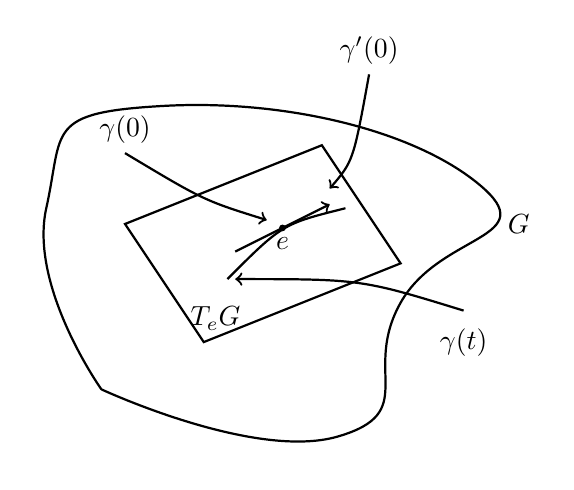
\begin{tikzpicture}
		
		% Draw the manifold G
		\draw[thick] plot [smooth,tension=1] 
		coordinates {(0.2,1.4) (3.2,0.8) (4,2.5) (5,4) (1,5) (-0.5,3.7) (0.2,1.4)};
		%\draw[thick] (0,0) to[out=30, in=180] (4,2.5) to[out=0, in=270] (5,4) to[out=90, in=30] (1,5) to[out=210, in=150] cycle;
		
		% Label G
		\node at (5.5,3.5) {$G$};
		
		% Draw the tangent space T_eG
		\draw[thick] (1.5, 2) -- (4, 3) -- (3, 4.5) -- (0.5, 3.5) -- cycle;
		
		% Label TeG
		\node at (1.65, 2.3) {$T_e G$};
		
		% Draw the curve \gamma(t)
		\draw[thick] (1.8, 2.8) .. controls (2.5, 3.5) .. (3.3, 3.7);
		
		% Label points and vectors
		\node at (0.5,4.7) {$\gamma(0)$};
		\draw[thick, ->] (0.5,4.4) .. controls (1.5,3.8) .. (2.3,3.55);
		\node at (4.8, 2) {$\gamma(t)$};
		\draw[thick, ->] (4.8,2.4) .. controls (3.5,2.8) .. (1.9,2.8);
		\filldraw[black] (2.5,3.45) circle (1pt) node[anchor=north] {$e$};
		\draw[thick, ->] (1.9, 3.15) -- (3.1, 3.75);
		\node at (3.6, 5.7) {$\gamma'(0)$};
		\draw[thick, ->] (3.6, 5.4) .. controls (3.4,4.3) .. (3.1,3.95);
		
	\end{tikzpicture}
\end{figure}
由解的形式可见,对于$G$在幺元处的切空间$T_eG$的任意一个向量$A=\gamma'(0)$,就有$G$中的一元素$\gamma(1)=\exp(\gamma'(0))$与之对应.现在我们稍微总结一下:对于李群$G$这个流形,我们可以找到其单参数子群$T_eG$作为其切空间,并且我们可以找到一个指数映射从切空间到原空间,很快,当我们学会李代数的时候,我们会再次使用李代数的语言来总结:``李代数就是李群的切空间所导出的代数".

我们再次回到群$G$和它的单参数子群,我们发现,如果给定$G$中与幺元邻近的一个元素\footnote{当然,由于我们研究线性群,幺元为单位矩阵.}$g$,并定义向量$A=\log g$,则由$e^A=g$ 知,$A$ 为$G$ 在$e$ 处之切向量,$e^tA$为以 $A$ 为单位切向量的单参数子群.因此,对$G$ 中与幺元$e$ 邻近的一个元素就有$T_{e}(G)$($G$ 在幺元处的切空间)中一向量$A$ 与之对应,也就是说,设$U\subset G$ 中包含$e$ 的一个适当邻域,我们建立了一种对应关系
\begin{equation}
	\begin{aligned}
		G\supset U&\overunderset{\log}{\exp}{\longleftrightarrow}T_{e}(G)\\g&\to A=\log g\\e^{A}&\leftarrow A
	\end{aligned}
\end{equation}
这种对应关系可以使我们对李群的研究转化到与其对应的在幺元$e$处的切空间$T_e(G)$.而我们知道,$T_e(G)$是由向量组成的线性空间,其线性结构具有先天优势,拥有远比李群简单的结构和运算.但由于我们前面所提到的,由于矩阵乘法相比于数乘的不可交互性,自然由此导出的切空间的运算自然也不能简单用普通加减法来表述,即如下关系
\begin{equation}
	\begin{aligned}&T_{e}(G)\qquad G\\&A\quad\longrightarrow\quad e^{A}\\&B\quad\longrightarrow\quad e^{B}\\&A+B\to e^{A+B}\ne e^{A}e^{B}\end{aligned}
\end{equation}
为此,我们迫切需要引入一种新的代数结构来反映$G$中的不可交换性,而具有这种新结构的线性空间$T_e(G)$
,就是我们下一节所要讲的\textbf{李代数}.
\section{李群与李代数}
\subsection{李代数}
由上面的讨论,我们现在知道$e^Ae^B\ne e^{A+B}$,那么,问题自然变为:$e^Ae^B=e^{?}$,或者表述为,$G$的单参数子群的代数结构是什么样的?

为了解决这个问题,我们设$A,B\in T_e(G)$,取一个参数$t$,并要求$|t|$适当小,从而能够保证$e^{tA}$与$e^{tB}$均为李群$G$中与幺元$e$邻近的元素\footnote{这个要求是必要的,我们需要满足后续使用级数的收敛性.}.现在我们构造一个函数:
\begin{equation}
	g(t)=e^{tA}e^{tB}e^{-tA}e^{-tB}
\end{equation}
显然,对于特例,即如果$e^{tA}$与$e^{tB}$可交换,$g(t)=e=\textbf{1}$,对于不可交换的情况,$g(t)$与幺元$e$的偏离程度反映了$e^{tA}$与$e^{tB}$的乘法与可交换的乘法之间的差异大小.现在我们具体分析$g(t)$.
\begin{equation}
	\begin{aligned}
		g(t)& =e^{tA}e^{tB}e^{-tA}e^{-tB} \\
		&=(\textbf{1}+tA+\frac{t^{2}}{2!}A^{2}+\frac{t^{3}}{3!}A^{3}+\cdots)(\textbf{1}+tB+\frac{t^{2}}{2!}B^{2}+\frac{t^{3}}{3!}B^{3}+\cdots) \\
		&(\textbf{1}-tA+\frac{t^2}{2!}A^2-\frac{t^3}{3!}A^3+\cdots)(\textbf{1}-tB+\frac{t^2}{2!}B^2-\frac{t^3}{3!}B^3+\cdots) \\
		&=\{\textbf{1}+t(A+B)+t^{2}(\frac{A^{2}}{2}+AB+\frac{B^{2}}{2})+t^{3}(\frac{A^{3}}{6}+\frac{A^{2}B}{2}+\frac{AB^{2}}{2}+\frac{B^{3}}{6})+O(t^{4})\} \\
		&\{\textbf{1}-t(A+B)+t^2(\frac{A^2}{2}+AB+\frac{B^2}{2})-t^3(\frac{A^3}{6}+\frac{A^2B}{2}+\frac{AB^2}{2}+\frac{B^3}{6})+O(t^4)\} \\
		&=\textbf{1}+t(A+B-A-B)+t^{2}(AB-BA)+t^{3}(\frac{A^{2}B}{2}-\frac{AB^{2}}{2}- \\
		&-\frac{B^2A}{2}+\frac{BA^2}{2}-ABA+BAB)+O(t^4) \\
		&=\textbf{1}+t^{2}[A,B]+\frac{t^{3}}{2}([A,[A,B]]-[B,[B,A]])+O(t^{4})
	\end{aligned}
\end{equation}
这里我们使用了对易子记号$[,]$,不过对于李代数,它也称为李括号,李乘法\footnote{事实上,对于线性群它等同于对易子,后面会加以区分的使用对易子和李括号.}.对于函数$g(t)$,我们有
\begin{equation}
	\frac{g(t)-\textbf{1}}{t^2}=[A,B]+O(t)
\end{equation}
因此,考虑极限$t\to0$时,
\begin{equation}
	\lim_{t\to0}\frac{g(t)-\textbf{1}}{t^{2}}=[A,B]
\end{equation}
由此,我们发现李群$G$的元素$e^{tA}$与$e^{tB}$的乘法的不可交换程度在$|t|$很小时主要取决于$[A,B]$

现在我们做变量代换$t=\sqrt{s}$,则
\begin{equation}
	\frac{g(\sqrt{s})-g(0)}{s}=[A,B]+O(\sqrt{s})
\end{equation}
并因此
\begin{equation}
	\lim_{s\to0}\frac{g(\sqrt{s})-g(0)}{s}=[A,B]
\end{equation}
这也说明$[A,B]$是李群$G$中过幺元的曲线$g(\sqrt{s})$在幺元处的\textbf{切向量},即$[A,B]\in T_e(G)$,这也意味着我们证明了如下关系
\begin{equation}
	\forall A,B\in T_{e}(G) , [A,B]\in T_{e}(G)
\end{equation}
即对易子(李括号)对向量空间$T_e(G)$的封闭性.


此时,我们可以回答开头所提到的问题了,不妨设$e^{tA}e^{tB}=e^{tC}$,则
\begin{equation}
	\begin{aligned}
		tC&=\log e^{tC}=\log e^{tA}e^{tB}\\
		&=\log\{(\textbf{1}+t(A+B)+\frac{t^{2}}{2}(A^{2}+2AB+B^{2})+ \\
		&\quad+\frac{t^{3}}{6}(A^{3}+3A^{2}B+3AB^{2}+B^{3})+O(t^{4})\} \\
		&=t(A+B)+\frac{t^{2}}{2}(A^{2}+2AB+B^{2})+\frac{t^{3}}{6}(A^{3}+3A^{2}B+3AB^{2}+B^{3})+O(t^{4}) \\
		&\quad-\{t(A+B)+\frac{t^2}{2}(A^2+2AB+B^2)+O(t^3)\}^2/2+ \\
		&\quad+\{t(A+B)+\frac{t^{2}}{2}(A^{2}+2AB+B^{2})+O(t^{3})\}^{3}/3+O(t^{4}) \\
		&=t(A+B)+\frac{t^{2}}{2}(AB-BA)+\frac{t^{3}}{12}(A^{2}B-ABA-ABA+BA^{2} \\
		&\quad-B^2A+BAB+BAB-AB^2)+O(t^4) \\
		&=(tA+tB)+\frac{1}{2}[tA,tB]+\frac{1}{12}[tA,[tA,tB]-tB,[tB,tA]]+O(t^{4}) 
	\end{aligned}
\end{equation}
由此可见,只要给出李括号,$T_e(G)$中知道了与$e^{tA},e^{tB}$相对应的元素$tA,tB$即可求得$T_e(G)$中与$e^{tA}e^{tB}$相对应的元素.因此,我们认为李括号可以表述李群切空间的代数结构,并对于李括号有下列性质(事实上完全类似在第一章给出过的对于对易子的同样性质).
\begin{equation}
	\begin{gathered}
		\left\lbrack {A, A}\right\rbrack = 0\\
		\left\lbrack {A, B}\right\rbrack = - \left\lbrack {B, A}\right\rbrack\\
		\left\lbrack {A, c}\right\rbrack = 0\;\left( {c\text{ 只是一个数 }}\right)\\
		\left\lbrack {A + B, C}\right\rbrack = \left\lbrack {A, C}\right\rbrack + \left\lbrack {B, C}\right\rbrack\\
		\left\lbrack {A,{BC}}\right\rbrack = \left\lbrack {A, B}\right\rbrack C + B\left\lbrack {A, C}\right\rbrack\\
		\left\lbrack {A,\left\lbrack {B, C}\right\rbrack }\right\rbrack + \left\lbrack {B,\left\lbrack {C, A}\right\rbrack }\right\rbrack + \left\lbrack {C,\left\lbrack {A, B}\right\rbrack }\right\rbrack = 0
	\end{gathered}
\end{equation}

我们称有了李括号的向量空间$T_e(G)$构成一个李代数,更准确的来讲是李群$G$的李代数,并记为$\mathfrak{g}$.\\
李群的李代数完全刻画了李群在幺元附近的结构,而要研究李群在幺元附近的性质只需要研究李代数即可,但是需要注意的是,李代数\textbf{仅}刻画了李群在幺元附近的\textbf{局部}性质,\textbf{不能}反映其整体性质,一个李群对应一个李代数,而一个李代数可以对应多个李群.
\begin{definition}[结构常数]
	设$G$是一个$r$维李群,取定幺元$e$的一个邻域$U$,在$U$中取定坐标系$\{U,\varphi\}$并取$e$为坐标原点:
	\begin{equation}
		\varphi(e)=(0,0,\cdots,0)
	\end{equation}
	对于其的单参数子群,我们有
	\begin{equation}
		\begin{cases}\gamma_j(t),&j=1,2,\cdots,r\\\varphi(\gamma_j(t))=(\underbrace{0,\cdots,0}_{(j-1)\text{个零}},t,0,\cdots,0)\end{cases}
	\end{equation}
	为其$r$条坐标曲线.
	
	以$X_{j}= \gamma _{j}^{\prime }(0),j= 1, 2, \cdots , r$记为其在幺元处的切向量.即$X_j\in T_e(G) = \mathfrak{g}, j= 1, 2, \cdots , r$.显然,$\{X_1,X_2,\cdots,X_r\}$可取作为向量空间$T_{_e}(G)$的基——$T_{e}(G)$中任一向量可用它们的线性组合表出.由于$[X_i,X_j]\in \mathfrak{g}$,所以
	\begin{equation}
		[X_{i},X_{j}]=\sum_{j,k=1}^{n}C_{ij}^{k}X_{k}\quad i,j=1,2,\cdots,r
	\end{equation}
	这$r^3$个数$\{C_{ij}^k\}k,i,j=1,2,\cdots,r$称为李群以$\{X_1,X_2,\cdots,X_r\}$,为基的\underline{结构常数}.
\end{definition}
对于李代数$\mathfrak{g}$中任意向量$X,Y$,有
\begin{equation}
	\begin{aligned}
		X&=\sum_{j=1}^{r}\xi^{j}X_{j}&Y=\sum_{j=1}^{r}\eta^{j}X_{j}\\
		X&\sim(\xi^{1},\xi^{2},\cdots,\xi^{r})&Y=(\eta^{1},\eta^{2},\cdots\eta^{r})\\
		Z&=[X,Y]=\left[\sum_{j=1}^{r}\xi^{j}X_{j},\sum_{k=1}^{r}\eta^{k}X_{k}\right]&=\sum_{i=1}^{r}\sum_{j,k=1}^{r}C_{jk}^{i_{k}}\xi^{j}\eta^{k}X_{i}
	\end{aligned}
\end{equation}
将$Z$也用坐标表示
\begin{equation}
	Z=\sum_{i=1}^{r}\zeta^{ i}X_{i},\quad Z\sim(\zeta^{ 1},\zeta^{ 2},\cdots\zeta^{ r})
\end{equation}
此时易求出结构常数
\begin{equation}
	\zeta^{i}=\sum_{j,k=1}^{r}C_{jk}^{i}\xi^{j}\eta^{k},\quad i=1,2,\cdots,r
\end{equation}
由此可见,结构常数可以完全确定一个李代数.

需要强调的是,结构常数与基的选取有关,而李代数的一个重要的问题就是如何选取适当的基使结构常数最简单.\\
或许到此,你可能还对结构常数一头雾水,在再次讲解结构常数之前,我们还是先给出一些基本性质,并实际算一下结构常数.
\begin{equation}
	\begin{aligned}
		&C_{ij}^{ k}=-C_{ji}^{ k}&i,j,k=1,2,\cdots,r\\
		&\sum_{l=1}^{r}\left(C_{ij}^{l}C_{lk}^{m}+C_{jk}^{l}C_{li}^{m}+C_{ki}^{l}C_{lj}^{m}\right)=0&i,j,k,m=1,2,\cdots,r.\end{aligned}
\end{equation}
\begin{example}
	我们再次考虑由例题3.8给出的群$T_2=\Big\{\begin{bmatrix}e^{x_1}&x_2\\0&1\end{bmatrix}\Big|x_1,x_2\in\mathbb{R}\Big\}$,我们知道$\gamma_1(t)=\begin{bmatrix}e^t&0\\0&1\end{bmatrix} -\infty<t<\infty $与$\gamma_2(t)=\begin{bmatrix}1&t\\0&1\end{bmatrix} -\infty<t<\infty $是$T_2$的两个单参数子群,同时也是过幺元的两条曲线,我们给出在幺元处的切向量$X_1=\gamma_1'(0)=\begin{bmatrix}1&0\\0&0\end{bmatrix},X_2=\gamma_2'(0)=\begin{bmatrix}0&1\\0&0\end{bmatrix}$,因此李群$T_2$的李代数$\mathfrak{t}_2$的基由$X_1,X_2$组成,现在来求结构常数.
	\begin{equation}
		\begin{aligned}&[X_1,X_1]=\begin{bmatrix}0&0\\0&0\end{bmatrix}\quad[X_2,X_2]=\begin{bmatrix}0&0\\0&0\end{bmatrix}\\&[X_1,X_2]=\begin{bmatrix}1&0\\0&0\end{bmatrix}\begin{bmatrix}0&1\\0&0\end{bmatrix}-\begin{bmatrix}0&1\\0&0\end{bmatrix}\begin{bmatrix}1&0\\0&0\end{bmatrix}=\begin{bmatrix}0&1\\0&0\end{bmatrix}=X_2.\end{aligned}
	\end{equation}
	所以,$C_{11}^1=C_{11}^2=C_{22}^1=C_{22}^2=0,\quad C_{12}^1=-C_{21}^1=0,\quad C_{12}^2=1,\quad C_{21}^2=-1.$
\end{example}
\begin{example}
	我们再次回到$SO(3)$群,现在我们来求其李代数$\mathfrak{so}(3)$及其结构常数.\\
	我们列出其群元(绕$x,y,z$的转动)
	\begin{equation}
		g_{x}(t)=\begin{bmatrix}1&0&0\\0&\cos t&-\sin t\\0&\sin t&\cos t\end{bmatrix},\quad g_y(t)=\begin{bmatrix}\cos t&0&\sin t\\0&1&0\\-\sin t&0&\cos t\end{bmatrix},\quad g_{z}(t)=\begin{bmatrix}\cos t&-\sin t&0\\\sin t&\cos t&0\\0&0&1\end{bmatrix}.
	\end{equation}
	此时,我们发现,这是其的三个单参数子群,而它们在幺元处的切向量一并给出
	\begin{equation}
		I_{1}=g_{x}'(0)=\begin{bmatrix}0&0&0\\0&0&-1\\0&1&0\end{bmatrix},\quad I_{2}=g_{y}'(0)=\begin{bmatrix}0&0&1\\0&0&0\\-1&0&0\end{bmatrix},\quad I_{3}=g_{z}'(0)=\begin{bmatrix}0&-1&0\\1&0&0\\0&0&0\end{bmatrix}.
	\end{equation}
	于是$\{I_1,I_2,I_3\}$构成$SO(3)$的李代数$\mathfrak{so}(3)$的一组基,其李括号为:
	\begin{equation}
		[I_1,I_2]=I_1I_2-I_2I_1=I_3,[I_2,I_3]=I_1,[I_3,I_1]=I_2
	\end{equation}
	同时得出结构常数$C_{12}^{ 1}=0,C_{12}^{ 2}=0,C_{12}^{ 3}=1,\cdots.$
	
	我们可以发现,对于这个李括号,其还等价于三维欧式空间的向量乘法,我们就得到了简单情况下的李括号的退化情况.
\end{example}
\subsection{李氏三定理和无穷小变换}
1
\subsection{李群的无穷小生成元}
1
\subsection{典型李群和李代数}
1

\section{角动量理论}
\subsection{量子力学中的无穷小转动} 

到此为止,我们还没有用到量子力学概念. 矩阵 $R$ 只是一个 $3 \times 3$ 的正交矩阵,它作用于写成列矩阵形式的矢量 $\mathbf{V}$ 上. 现在我们必须弄懂如何表征量子力学中的转动.

因为转动影响物理系统, 预期转动后系统的态右矢与原来未经转动系统的态右矢有所不同. 给定由一个 $3 \times 3$ 正交矩阵 $R$ 表征的一个转动算符 $R$ ,我们将其与适当的右矢空间里的一个算符 $\mathcal{D}\left( R\right)$ 这样联系起来,使得:

$$
|\alpha {\rangle }_{R} = \mathcal{D}\left( R\right) |\alpha \rangle , tag{3.1.10}
$$

其中 ${\left| \alpha \right\rangle }_{R}$ 和 $|\alpha \rangle$ 分别代表转动后系统和原始系统的右矢**. 注意, $3 \times 3$ 正交矩阵 $R$ 作用在一个由经典矢量的三个分量构成的一个列矩阵上,然而,算符 $\mathcal{D}\left( R\right)$ 作用在右矢空间的态矢量上. $\mathcal{D}\left( R\right)$ 的矩阵表示一将在随后几节非常详细地研究——依赖所涉及的特定的右矢空间的维数 $N$ . 对于 $N = 2$ ,适用于描写没有其他自由度的自旋 $\frac{1}{2}$ 系统, $\mathcal{D}\left( R\right)$ 用一个 2 $\times 2$ 矩阵表示; 而对于自旋为 1 的系统,适当的表示是一个 $3 \times 3$ 的幺正矩阵,等等.

---

* 在基础力学中有一个熟悉的例子. 角速度矢量 $\omega$ ,它表征转动角在一个无穷小时间间隔内的一个无穷小改变. 遵从矢量加法的通常规则, 包括矢量加法的交换性. 然而, 我们不能认为一个有限的角变化具有这一矢量性质.

** 符号 $\mathcal{D}$ 来自德文的 Drehung,意思是 “转动”.

---

要构建转动算符 $\mathcal{D}\left( R\right)$ ,最有成效的方法仍然是先考查它在一个无穷小转动下的性质. 我们几乎可以猜到必须怎样通过类比来进行. 在我们于 1.6 节和 2.1 节分别研究的平移与时间演化这两种情况下,适用的无穷小算符都可以用一个厄米算符 $G$ 写成

$$
{U}_{\varepsilon } = 1 - {iG\varepsilon } tag{3.1.11}
$$

具体说来,对于沿 $x$ 方向位移 $d{x}^{\prime }$ 的无穷小平移取

$$
G \rightarrow \frac{{p}_{x}}{\hslash },\;\varepsilon \rightarrow d{x}^{\prime } tag{3.1.12}
$$

而对于时间平移 ${dt}$ 的无穷小时间演化取

$$
G \rightarrow \frac{H}{h},\;\varepsilon \rightarrow {dt} tag{3.1.13}
$$

由经典力学我们知道角动量是转动的生成元, 就像动量和哈密顿量分别为平移与时间演化的生成元一样. 因此,我们以这样的方式来定义角动量算符 ${J}_{k}$ ,通过在 (3.1.11) 式中让

$$
G \rightarrow \frac{{J}_{k}}{\hslash },\;\varepsilon \rightarrow {d\phi } tag{3.1.14}
$$

得到一个绕第 $k$ 个轴转 ${d\phi }$ 角的无穷小转动算符. 若 ${J}_{k}$ 是厄米的,无穷小转动算符保证是幺正的,而且在 ${d\phi } \rightarrow 0$ 的极限下约化为单位算符. 更普遍地,对一个绕着由单位矢量 $\widehat{\mathbf{n}}$ 表征的方向转无穷小 ${d\phi }$ 角的转动,我们有

$$
\mathcal{D}\left( {\widehat{\mathbf{n}},{d\phi }}\right) = 1 - i\left( \frac{\mathbf{J} \cdot \widehat{\mathbf{n}}}{\hslash }\right) {d\phi } tag{3.1.15}
$$

在本书中,我们强调并没有把角动量算符定义为 $\mathbf{x} \times \mathbf{p}$ . 这一点很重要,因为自旋角动量一一我们的普遍形式也适用于它一一与 ${x}_{i}$ 和 ${p}_{j}$ 毫无关系. 换个方式讲,在经典力学中,可以证明定义为 $\mathbf{x} \times \mathbf{p}$ 的角动量是转动的生成元; 相比之下,在量子力学中我们定义 $\mathbf{J}$ 使得一个无穷小转动算符取 (3.1.15) 式形式.

一个有限转动可以通过组合相继地绕同一个轴的无穷小转动得到. 例如, 如果我们对于一个绕 $z$ 轴转 $\phi$ 角的有限转动感兴趣,我们考虑

$$
{\mathcal{D}}_{z}\left( \phi \right) = \mathop{\lim }\limits_{{N \rightarrow \infty }}{\left\lbrack 1 - i\left( \frac{{J}_{z}}{\hslash }\right) \left( \frac{\phi }{N}\right) \right\rbrack }^{N}
$$

$$
= \exp \left( \frac{-i{J}_{z}\phi }{\hslash }\right) tag{3. 1.16}
$$

$$
= 1 - \frac{i{J}_{z}\phi }{\hslash } - \frac{{J}_{z}^{2}{\phi }^{2}}{2{\hslash }^{2}} + \cdots .
$$

为了求得角动量对易关系, 我们还需要一个概念. 正如我们前面评注的, 对每个用 3 $\times 3$ 正交矩阵 $R$ 表示的转动 $R$ ,在恰当的右矢空间中都存在一个转动算符 $\mathcal{D}\left( R\right)$ . 我们进一步假设 $\mathcal{D}\left( R\right)$ 与 $R$ 有相同的群性质

$$
\text{单位元:}R \cdot 1 = R \Rightarrow \mathcal{D}\left( R\right) \cdot 1 = \mathcal{D}\left( R\right) tag{3.1.17a}
$$

封闭性: ${R}_{1}{R}_{2} = {R}_{3} \Rightarrow \mathcal{D}\left( {R}_{1}\right) \mathcal{D}\left( {R}_{2}\right) = \mathcal{D}\left( {R}_{3}\right)$(3.1.17b)

逆: $R{R}^{-1} = 1 \Rightarrow \mathcal{D}\left( R\right) {\mathcal{D}}^{-1}\left( R\right) = 1$

(3.1. ${17}\mathrm{c}$ )

$$
{R}^{-1}R = 1 \Rightarrow {\mathcal{D}}^{-1}\left( R\right) \mathcal{D}\left( R\right) = 1
$$

$$
\text{结合律:}{R}_{1}\left( {{R}_{2}{R}_{3}}\right) = \left( {{R}_{1}{R}_{2}}\right) {R}_{3} = {R}_{1}{R}_{2}{R}_{3}
$$

$$
\Rightarrow \mathcal{D}\left( {R}_{1}\right) \left\lbrack {\mathcal{D}\left( {R}_{2}\right) \mathcal{D}\left( {R}_{3}\right) }\right\rbrack tag{3.1.17d}
$$

$$
= \left\lbrack {\mathcal{D}\left( {R}_{1}\right) \mathcal{D}\left( {R}_{2}\right) }\right\rbrack \mathcal{D}\left( {R}_{3}\right)
$$

$$
= \mathcal{D}\left( {R}_{1}\right) \mathcal{D}\left( {R}_{2}\right) \mathcal{D}\left( {R}_{3}\right) .
$$

现在让我们返回到基于 $R$ 矩阵写成的转动操作 (3.1.9) 式的基本对易关系. 它的转动算符类似公式为

$$
\left( {1 - \frac{i{J}_{x}\varepsilon }{\hslash } - \frac{{J}_{x}^{2}{\varepsilon }^{2}}{2{\hslash }^{2}}}\right) \left( {1 - \frac{i{J}_{y}\varepsilon }{\hslash } - \frac{{J}_{y}^{2}{\varepsilon }^{2}}{2{\hslash }^{2}}}\right) tag{3. 1.18}
$$

$$
- \left( {1 - \frac{i{J}_{y}\varepsilon }{\hslash } - \frac{{J}_{y}^{2}{\varepsilon }^{2}}{2{\hslash }^{2}}}\right) \left( {1 - \frac{i{J}_{x}\varepsilon }{\hslash } - \frac{{J}_{x}^{2}{\varepsilon }^{2}}{2{\hslash }^{2}}}\right) = 1 - \frac{i{J}_{z}{\varepsilon }^{2}}{\hslash } - 1.
$$

$\varepsilon$ 量级的项已自动地消掉了. 让 (3.1.18) 式两边的 ${\varepsilon }^{2}$ 量级的项相等,我们得到

$$
\left\lbrack {{J}_{x},{J}_{y}}\right\rbrack = i\hslash {J}_{z}, tag{3.1.19}
$$

将这种做法重复用于绕其他轴的转动可得到

$$
\left\lbrack {{J}_{i},{J}_{j}}\right\rbrack = i\hslash {\varepsilon }_{ijk}{J}_{k}, tag{3.1.20}
$$

该式称为角动量的基本对易关系.

一般说来, 当无穷小变换的生成元不对易时, 相应操作的群称为非阿贝尔群. 基于 (3.1.20)式, 三维转动群是非阿贝尔的. 相比之下, 三维平移群是阿贝尔的, 因为即使 $i \neq j,{p}_{i}$ 和 ${p}_{j}$ 也是对易的.

注意在获得对易关系 (3.1.20) 时, 使用了以下两个概念

1. ${J}_{k}$ 是绕第 $k$ 轴转动的生成元.

2. 绕不同轴的转动不对易.

毫不夸张地说, 对易关系 (3.1.20) 式以一种紧凑的方式归纳了三维转动的一切基本性质.

\subsection{自旋$\frac{1}{2}$的转动算符}

角动量对易关系 (3.1.20) 可以实现的最低维数 $N = 2$ . 在第 1 章的习题 1.8 中读者已经核对过. 由

$$
{S}_{x} = \left( \frac{\hslash }{2}\right) \{ \left( {\left| {+\rangle \langle - }\right| ) + \left( \left| {-\rangle \langle + }\right| \right) \} }\right) ,
$$

$$
{S}_{y} = \left( \frac{i\hslash }{2}\right) \{ - \left( {\left| {+\rangle \langle - }\right| ) + \left( \left| {-\rangle \langle + }\right| \right) \} }\right) , tag{3.2.1}
$$

$$
{S}_{z} = \left( \frac{\hslash }{2}\right) \{ \left( {\left| {+\rangle \langle + }\right| ) - \left( \left| {-\rangle \langle - }\right| \right) \} }\right)
$$

定义的算符满足把 ${J}_{k}$ 换成 ${S}_{k}$ 的对易关系 (3.1.20) 式. 自然界利用 (3.1.20) 式的最低维实现不是先验显然的, 但许多实验——从原子光谱到核磁共振——足以让我们相信这就是实际的情况.

考虑一个绕 $z$ 轴转有限角度 $\phi$ 的转动. 如果一个自旋 $\frac{1}{2}$ 系统的右矢在转动前由 $|\alpha \rangle$ 给定, 则转动后的右矢为

$$
|\alpha {\rangle }_{R} = {\left. {D}_{z}\left( \phi \right) \right| }_{\alpha }\rangle tag{3.2.2}
$$

其中

$$
{\mathcal{D}}_{z}\left( \phi \right) = \exp \left( \frac{-i{S}_{z}\phi }{\hslash }\right) . tag{3.2.3}
$$

为了看到这个算符真的转动了这个物理系统,让我们看一看它对于 $\left\langle {S}_{x}\right\rangle$ 的影响. 转动之下这个期待值变化如下

$$
\left\langle {S}_{x}\right\rangle { \rightarrow }_{R}\left\langle {\alpha \left| {S}_{x}\right| \alpha }\right\rangle {}_{R} = \left\langle {\alpha \left| {{\mathcal{D}}_{z}^{ \dagger }\left( \phi \right) {S}_{x}{\mathcal{D}}_{z}\left( \phi \right) }\right| \alpha }\right\rangle , tag{3.2.4}
$$

因此我们必须计算

$$
\exp \left( \frac{i{S}_{z}\phi }{\hslash }\right) {S}_{x}\exp \left( \frac{i{S}_{z}\phi }{\hslash }\right) . tag{3. 2.5}
$$

为了教学原因, 我们用两种不同的方法计算它.

推导 1: 这里我们使用由 (3.2.1) 式给出的 ${S}_{x}$ 的具体形式. 于是对 (3.2.5) 式,我们得到

$$
\left( \frac{\hslash }{2}\right) \exp \left( \frac{i{S}_{z}\phi }{\hslash }\right) \{ \left( {\left| {+\rangle \langle - }\right| ) + \left( \left| {-\rangle \langle + }\right| \right) }\right) \} \exp \left( \frac{i{S}_{z}\phi }{\hslash }\right)
$$

$$
= \left( \frac{\hslash }{2}\right) \left( {{e}^{{i\phi }/2}\left| {+\rangle \left\langle {-\left| {{e}^{{i\phi }/2} + {e}^{-{i\phi }/2}}\right| - }\right\rangle \langle + }\right| {e}^{-{i\phi }/2}}\right) tag{3.2.6}
$$

$$
= \frac{\hslash }{2}\left\lbrack {\{ \left( {\left| {+\rangle \langle - }\right| ) + \left( {\left| {-\rangle \langle + }\right| )}\right) \cos \phi + i\{ \left( {\left| {+\rangle \langle - }\right| ) - \left( {\left| {-\rangle \langle + }\right| )}\right) \sin \phi }\right) }\right) }\right\rbrack
$$

$$
= {S}_{x}\cos \phi - {S}_{y}\sin \phi .
$$

推导 2: 换一种做法, 我们可以使用 (2.3.47) 式计算 (3.2.5) 式:

$$
\exp \left( \frac{i{S}_{z}\phi }{\hslash }\right) {S}_{x}\exp \left( \frac{-i{S}_{z}\phi }{\hslash }\right) = {S}_{x} + \left( \frac{i\phi }{\hslash }\right) \underset{{ih}{S}_{y}}{\underbrace{\left\lbrack {S}_{z},{S}_{x}\right\rbrack }}
$$

$$
+ \left( \frac{1}{2!}\right) {\left( \frac{i\phi }{\hslash }\right) }^{2}\underset{{h}^{2}{S}_{x}}{\underbrace{\left\lbrack {S}_{z},\underset{i\hslash {S}_{y}}{\underbrace{\left\lbrack {S}_{z},{S}_{x}\right\rbrack }}\right\rbrack }} + \left( \frac{1}{3!}\right) \underset{{h}^{3}{S}_{x}}{\underbrace{\left( \frac{i\phi }{\hslash }\right. }}\underset{i{h}^{3}{S}_{y}}{\underbrace{\left\lbrack {S}_{z},\underset{{h}^{2}{S}_{x}}{\underbrace{\left\lbrack {S}_{z},\left\lbrack {S}_{x},\left\lbrack {S}_{x}\right\rbrack \right\rbrack \right\rbrack }}\right\rbrack }} + \cdots
$$

$$
= {S}_{x}\left\lbrack {1 - \frac{{\phi }^{2}}{2!} + \cdots }\right\rbrack - {S}_{y}\left\lbrack {\phi - \frac{{\phi }^{3}}{3!} + \cdots }\right\rbrack
$$

$$
= {S}_{x}\cos \phi - {S}_{y}\sin \phi . tag{3.2.7}
$$

注意,在推导 2 中我们只用到了 ${S}_{i}$ 的对易关系,所以这个方法可被推广到角动量高于 $\frac{1}{2}$ 的系统的转动.

对于自旋 $\frac{1}{2}$ ,这两种方法都给出

$$
\left\langle {S}_{x}\right\rangle { \rightarrow }_{R}\left\langle {\alpha \left| {S}_{x}\right| \alpha }\right\rangle {}_{R} = \left\langle {S}_{x}\right\rangle \cos \phi - \left\langle {S}_{y}\right\rangle \sin \phi , tag{3.2.8}
$$

其中, 无下标的期待值被理解为是对 (老的) 未转动的系统取的. 类似地,

$$
\left\langle {S}_{y}\right\rangle \rightarrow \left\langle {S}_{y}\right\rangle \cos \phi + \left\langle {S}_{x}\right\rangle \sin \phi . tag{3.2.9}
$$

至于 ${S}_{z}$ 的期待值,由于 ${S}_{z}$ 与 ${\mathcal{D}}_{z}\left( \phi \right)$ 对易,因而无变化

$$
\left\langle {S}_{z}\right\rangle \rightarrow \left\langle {S}_{z}\right\rangle . tag{3. 2.10}
$$

关系式 (3.2.8)、(3.2.9) 和 (3.2.10) 是十分合理的. 它们表明当转动算符 (3.2.3)

作用于态右矢时,它的确把 $\mathbf{S}$ 的期待值绕 $z$ 轴转动了 $\phi$ 角. 换句话说,自旋算符期待值的行为仿佛是在旋转

$$
\left\langle {S}_{k}\right\rangle \rightarrow \mathop{\sum }\limits_{l}{R}_{kl}\left\langle {S}_{l}\right\rangle , tag{3.2.11}
$$

之下的经典矢量,其中 ${R}_{kl}$ 是所涉及问题中确定转动的 $3 \times 3$ 正交矩阵 $R$ 的矩阵元. 从我们的推导 2 应该很清楚,这个性质不只限于自旋 $\frac{1}{2}$ 系统的自旋算符. 一般地说,在转动下, 我们有

$$
\left\langle {J}_{k}\right\rangle \rightarrow \mathop{\sum }\limits_{l}{R}_{kl}\left\langle {J}_{l}\right\rangle tag{3.2.12}
$$

其中 ${J}_{k}$ 是满足角动量对易关系 (3.1.20) 式的转动生成元. 稍后,将证明这种关系可以进一步推广到任何矢量算符.

至此每件事情都在预料之中. 但现在, 准备给你一个惊喜! 稍微仔细地考查一下转动算符 (3.2.3) 式在一般的态右矢

$$
\left| {\alpha \rangle = }\right| + \rangle \langle + \mid \alpha \rangle + \mid - \rangle \langle - \mid \alpha \rangle , tag{3.2.13}
$$

上的效应. 我们看到

$$
\exp \left( \frac{-i{S}_{z}\phi }{\hslash }\right) \left| {\alpha \rangle = {e}^{-{i\phi }/2}}\right| + \rangle \left\langle {+\left| {\alpha \rangle + {e}^{{i\phi }/2}}\right| - }\right\rangle \langle - \mid \alpha \rangle . tag{3.2.14}
$$

在这里,半角 $\phi /2$ 的出现具有一个很意思的后果.

让我们考虑一个转 ${2\pi }$ 角的转动. 那时我们有

$$
\left| {\alpha {\rangle }_{{R}_{{z}^{\left( 2\pi \right) }}} \rightarrow - }\right| \alpha \rangle \text{.} tag{3. 2.15}
$$

因此,转了 ${360}^{ \circ }$ 以后的态右矢与原来的右矢差了一个负号. 我们需要一个 ${720}^{ \circ }\left( {\phi = {4\pi }}\right)$ 的转动,才能回到具有正号的同样的右矢. 注意,对于 $\mathbf{S}$ 的期待值,这个负号消失了,因为 $\mathbf{S}$ 被 $|\alpha \rangle$ 和 $\langle \alpha \mid$ 夹在中间,而这两个右矢和左矢都改变了符号. 这个负号能被观测到吗? 在讨论自旋进动之后, 我们将给出这个有趣问题的答案.

\subsection{再谈自旋进动} 

现在用一种新的观点来处理在 2.1 节已经讨论过的自旋进动问题. 回想一下这个问题的基本哈密顿量为

$$
H = - \left( \frac{e}{{m}_{e}c}\right) \mathbf{S} \cdot \mathbf{B} = \omega {S}_{z}, tag{3.2.16}
$$

其中

$$
\omega \equiv \frac{\left| e\right| B}{{m}_{e}c}. tag{3.2.17}
$$

基于该哈密顿量的时间演化算符由

$$
u\left( {t,0}\right) = \exp \left( \frac{-{iHt}}{\hslash }\right) = \exp \left( \frac{-i{S}_{z}{\omega t}}{\hslash }\right) . tag{3. 2.18}
$$

给出. 把这个方程与 (3.2.3) 式比较,我们看到在 (3.2.3) 式中令 $\phi$ 等于 ${\omega t}$ ,这个时间演化算符就与 (3.2.3) 式中的转动算符精确地相同. 这样, 我们就可立即看到为什么这个哈密顿量引起自旋进动. 重新改写 (3.2.8) 式、 (3.2.9) 式和 (3.2.10) 式, 我们得到

$$
{\left\langle {S}_{x}\right\rangle }_{t} = {\left\langle {S}_{x}\right\rangle }_{t = 0}\cos {\omega t} - {\left\langle {S}_{y}\right\rangle }_{t = 0}\sin {\omega t},
$$

(3. ${2.19a}$ )

$$
{\left\langle {S}_{y}\right\rangle }_{t} = {\left\langle {S}_{y}\right\rangle }_{t = 0}\cos {\omega t} + {\left\langle {S}_{x}\right\rangle }_{t = 0}\sin {\omega t},
$$

(3. ${2.19}\mathrm{\;b}$ )

$$
{\left\langle {S}_{z}\right\rangle }_{t} = {\left\langle {S}_{z}\right\rangle }_{t = 0}.
$$

(3. ${2.19c}$ )

在 $t = {2\pi }/\omega$ 之后,自旋回到原始方向.

这组方程可以用于讨论一个 $\mathbf{\mu }$ 子的自旋进动,该粒子是一个类电子的粒子,其重量是电子的 210 倍. $\mu$ 子的磁矩可以从其他一些实验——例如, $\mu$ 子偶素,一个正的 $\mu$ 子与一个电子的束缚态的超精细分裂——确定,结果正如自旋 $\frac{1}{2}$ 粒子的狄拉克相对论理论所预期的那样为 $e\hslash /2{m}_{\mu }c$ . (在这里我们将忽略非常小的、来自量子场论效应的修正.) 知道了磁矩我们就能预言进动的角频率. 因此, (3.2.19) 式就可以, 事实上已经, 被实验检验 (见图 2.1). 实际上,当外磁场引起自旋进动时,可利用来自 $\mu$ 衰变的电子倾向于优先沿 $\mu$ 子自旋反方向发射来分析自旋的方向.

现在让我们来看一下态右矢自身的时间演化. 假定初始时 $\left( {t = 0}\right)$ 右矢由 (3.2.13) 式给定,在 $t$ 时刻之后我们得到

$$
\left| {\alpha ,{t}_{0} = 0;t}\right\rangle = {e}^{-{i\omega t}/2}\left| {+\rangle \left\langle {+ \mid \alpha }\right\rangle + {e}^{+{i\omega t}/2}}\right| - \rangle \langle - \mid \alpha \rangle . tag{3.2.20}
$$

表示式 (3.2.20) 在 $t = {2\pi }/\omega$ 得到了一个负号,我们必须等到 $t = {4\pi }/\omega$ 时才能回到有同样符号的原始的态右矢. 总之, 态右矢的周期是自旋进动周期的两倍长:

$$
{\tau }_{\text{进动 }} = \frac{2\pi }{\omega },
$$

(3. ${2.21a}$ )

$$
{\tau }_{\text{态右矢 }} = \frac{4\pi }{\omega }, tag{3.2.21b}
$$

\subsection{泡利二分量形式} 

利用泡利在 1926 年引入的二分量旋量形式,可以很方便地处理自旋 $\frac{1}{2}$ 系统的态右矢. 在 1.3 节我们学会了怎样使用一个列 (行) 矩阵表示一个右矢 (左矢); 我们所要做的是把基于某个指定基右矢的展开系数安排到一个列(行)矩阵中. 在自旋 $\frac{1}{2}$ 的情况下,对于基右矢和基左矢, 我们有

$$
\left| {+\rangle \doteq \left( \begin{array}{l} 1 \\ 0 \end{array}\right) \equiv {\chi }_{ + }\;}\right| - \rangle \doteq \left( \begin{array}{l} 0 \\ 1 \end{array}\right) \equiv {\chi }_{ - } tag{3.2.26}
$$

$$
\langle + \mid \doteq \left( {1,0}\right) = {\chi }_{ + }^{ \dagger }\;\langle - \mid \doteq \left( {0,1}\right) = {\chi }_{ - }^{ \dagger }
$$

和对一个任意的态右矢和相应的态左矢有

$$
\left| {\alpha \rangle = }\right| + \rangle \langle + \left| {\alpha \rangle + }\right| - \rangle \langle - \mid \alpha \rangle \doteq \left( \begin{array}{l} \langle + \mid \alpha \rangle \\ \langle - \mid \alpha \rangle \end{array}\right) tag{3.2.27a}
$$

和

$$
\langle \alpha \left| { = \langle \alpha }\right| + \rangle \langle + \left| {+\langle \alpha }\right| - \rangle \langle - | \doteq \left( {\langle \alpha \mid + \rangle ,\langle \alpha \mid - \rangle }\right) tag{3.2.27b}
$$

列矩阵 (3.2.27a) 式称为二分量旋量, 记为

$$
\chi = \left( \begin{array}{l} \langle + \mid \alpha \rangle \\ \langle - \mid \alpha \rangle \end{array}\right) \equiv \left( \begin{array}{l} {c}_{ + } \\ {c}_{ - } \end{array}\right)
$$

$$
= {c}_{ + }{\chi }_{ + } + {c}_{ - }{\chi }_{ - }, tag{3.2.28}
$$


其中 ${c}_{ + }$ 和 ${c}_{ - }$ 一般都是复数. 对于 ${\chi }^{ \dagger }$ 我们有

$$
{\chi }^{ \dagger } = \left( {\langle \alpha \mid + \rangle ,\langle \alpha \mid - \rangle }\right) = \left( {{c}_{ + }^{ * },{c}_{ - }^{ * }}\right) , tag{3.2.29}
$$

矩阵元 $\left\langle {\pm \left| {S}_{k}\right| + }\right\rangle$ 和 $\left\langle {\pm \left| {S}_{k}\right| - }\right\rangle$ ,除去 $\hslash /2$ 之外,被设定等于那些 $2 \times 2$ 的、以泡利矩阵著称的矩阵 ${\sigma }_{k}$ . 我们确定

$$
\left\langle {\pm \left| {S}_{k}\right| + }\right\rangle \equiv \left( \frac{\hslash }{2}\right) {\left( {\sigma }_{k}\right) }_{\pm , + },\;\left\langle {\pm \left| {S}_{k}\right| - }\right\rangle \equiv \left( \frac{\hslash }{2}\right) {\left( {\sigma }_{k}\right) }_{\pm , - }. tag{3. 2.30}
$$

现在我们可以用 $\chi$ 和 ${\sigma }_{k}$ 写出期待值 $\left\langle {S}_{k}\right\rangle$

$$
\left\langle {S}_{k}\right\rangle = \left\langle {\alpha \left| {S}_{k}\right| \alpha }\right\rangle = \mathop{\sum }\limits_{{{a}^{\prime } = + , - }}\mathop{\sum }\limits_{{{a}^{\prime \prime } = + , - }}\left\langle {\alpha \left| {a}^{\prime }\right\rangle \left\langle {{a}^{\prime }\left| {S}_{k}\right| {a}^{\prime \prime }}\right\rangle \left\langle {a}^{\prime \prime }\right| \alpha }\right\rangle tag{3. 2.31}
$$

$$
= \left( \frac{\hslash }{2}\right) {\chi }^{ \dagger }{\sigma }_{k}\chi
$$

其中在最后一行用到了矩阵乘法的常用规则. 显然我们可从 (3.2.1) 和 (3.2.30) 式看到

$$
{\sigma }_{1} = \left( \begin{array}{ll} 0 & 1 \\ 1 & 0 \end{array}\right) ,\;{\sigma }_{2} = \left( \begin{matrix} 0 & - i \\ i & 0 \end{matrix}\right) ,\;{\sigma }_{3} = \left( \begin{matrix} 1 & 0 \\ 0 & - 1 \end{matrix}\right) , tag{3. 2.32}
$$

其中下标 1,2 和 3 分别代表 $x, y$ 和 $z$ .

下面列出泡利矩阵的一些性质. 首先,

$$
{\sigma }_{i}^{2} = 1
$$

(3. ${2.33a}$ )

$$
{\sigma }_{i}{\sigma }_{j} + {\sigma }_{j}{\sigma }_{i} = 0,\;\text{ 对于 }i \neq j,
$$

(3. ${2.33}\mathrm{\;b}$ )

其中 (3.2.33a) 式的右边被理解为 $2 \times 2$ 单位矩阵. 当然,这两个关系式等价于反对易关系

$$
\left\{ {{\sigma }_{i},{\sigma }_{j}}\right\} = 2{\delta }_{ij}, tag{3. 2.34}
$$

还有对易关系

$$
\left\lbrack {{\sigma }_{i},{\sigma }_{j}}\right\rbrack = {2i}{\varepsilon }_{ijk}{\sigma }_{k}, tag{3. 2.35}
$$

可以看出,它显然就是角动量对易关系 (3.1.20) 的 $2 \times 2$ 矩阵实现. 比较 (3.2.34) 式和 (3.2.35) 式, 我们可以得到

$$
{\sigma }_{1}{\sigma }_{2} = - {\sigma }_{2}{\sigma }_{1} = i{\sigma }_{3}\cdots tag{3. 2.36}
$$

还要注意

$$
{\sigma }_{i}^{ \dagger } = {\sigma }_{i},
$$

(3. ${2.37a}$ )

$$
\det \left( {\sigma }_{i}\right) = - 1, tag{3. 2.37b}
$$

$$
\operatorname{Tr}\left( {\sigma }_{i}\right) = 0.
$$

(3. ${2.37}\mathrm{c}$ )

现在考虑 $\mathbf{\sigma } \cdot \mathbf{a}$ ,其中 $\mathbf{a}$ 是一个三维矢量. 要把这个量理解为实际上是一个 $2 \times 2$ 矩阵. 于是

$$
\mathbf{\sigma } \cdot \mathbf{a} \equiv \mathop{\sum }\limits_{k}{a}_{k}{\sigma }_{k}
$$

$$
= \left( \begin{matrix} + {a}_{3} & {a}_{1} - i{a}_{2} \\ {a}_{1} + i{a}_{2} & - {a}_{3} \end{matrix}\right) tag{3. 2.38}
$$

还有一个非常重要的恒等式

$$
\left( {\mathbf{\sigma } \cdot \mathbf{a}}\right) \left( {\mathbf{\sigma } \cdot \mathbf{b}}\right) = \mathbf{a} \cdot \mathbf{b} + i\mathbf{\sigma } \cdot \left( {\mathbf{a} \times \mathbf{b}}\right) . tag{3. 2.39}
$$

为证明该式, 所需的是反对易关系和对易关系, 它们分别为 (3.2.34) 式与 (3.2.35) 式:

$$
\mathop{\sum }\limits_{j}{\sigma }_{j}a\mathop{\sum }\limits_{k}{\sigma }_{k}{b}_{k} = \mathop{\sum }\limits_{j}\mathop{\sum }\limits_{k}\left( {\frac{1}{2}\left\{ {{\sigma }_{j},{\sigma }_{k}}\right\} + \frac{1}{2}\left\lbrack {{\sigma }_{j},{\sigma }_{k}}\right\rbrack }\right) {a}_{j}{b}_{k}
$$

$$
= \mathop{\sum }\limits_{j}\mathop{\sum }\limits_{k}\left( {{\delta }_{jk} + i{\varepsilon }_{jkl}{\sigma }_{l}}\right) {a}_{j}{b}_{k} tag{3. 2.40}
$$

$$
= \mathbf{a} \cdot \mathbf{b} + i\mathbf{\sigma } \cdot \left( {\mathbf{a} \times \mathbf{b}}\right) .
$$

如果 $\mathbf{a}$ 的分量都是实的,我们有

$$
{\left( \mathbf{\sigma } \cdot \mathbf{a}\right) }^{2} = {\left| \mathbf{a}\right| }^{2}, tag{3. 2.41}
$$

其中 $\left| \mathbf{a}\right|$ 是矢量 $\mathbf{a}$ 的长度.

\subsection{二分量形式中的转动}

现在研究转动算符 $\mathcal{D}\left( {\widehat{\mathbf{n}},\phi }\right)$ 的 $2 \times 2$ 矩阵表示. 如下

$$
\exp \left( \frac{-i\mathbf{S} \cdot \widehat{\mathbf{n}}\phi }{\hslash }\right) \doteq \exp \left( \frac{-i\mathbf{\sigma } \cdot \widehat{\mathbf{n}}\phi }{2}\right) . tag{3. 2.42}
$$

利用从 (3.2.41) 式得到的

$$
{\left( \mathbf{\sigma } \cdot \widehat{\mathbf{n}}\right) }^{n} = \left\{ \begin{array}{ll} 1 & \text{ 对于偶数的 }n, \\ \mathbf{\sigma } \cdot \widehat{\mathbf{n}} & \text{ 对于奇数的 }n, \end{array}\right. tag{3.2.43}
$$

我们可以写出

$$
\exp \left( \frac{-i\mathbf{\sigma } \cdot \widehat{\mathbf{n}}\phi }{2}\right) = \left\lbrack {1 - \frac{{\left( \mathbf{\sigma } \cdot \widehat{\mathbf{n}}\right) }^{2}}{2!}{\left( \frac{\phi }{2}\right) }^{2} + \frac{{\left( \mathbf{\sigma } \cdot \widehat{\mathbf{n}}\right) }^{4}}{4!}{\left( \frac{\phi }{2}\right) }^{4} - \cdots }\right\rbrack
$$

$$
- i\left\lbrack {\left( {\mathbf{\sigma } \cdot \widehat{\mathbf{n}}}\right) \frac{\phi }{2} - \frac{{\left( \mathbf{\sigma } \cdot \widehat{\mathbf{n}}\right) }^{3}}{3!}{\left( \frac{\phi }{2}\right) }^{3} + \cdots }\right\rbrack tag{3. 2.44}
$$

$$
= 1\cos \left( \frac{\phi }{2}\right) - i\mathbf{\sigma } \cdot \widehat{\mathbf{n}}\sin \left( \frac{\phi }{2}\right) .
$$

显然,以 $2 \times 2$ 形式我们有

$$
\exp \left( \frac{-i\mathbf{\sigma } \cdot \widehat{\mathbf{n}}\phi }{2}\right) = \left( \begin{array}{ll} \cos \left( \frac{\phi }{2}\right) - i{n}_{z}\sin \left( \frac{\phi }{2}\right) & \left( {-i{n}_{x} - {n}_{y}}\right) \sin \left( \frac{\phi }{2}\right) \\ \left( {-i{n}_{x} + {n}_{y}}\right) \sin \left( \frac{\phi }{2}\right) & \cos \left( \frac{\phi }{2}\right) + i{n}_{z}\sin \left( \frac{\phi }{2}\right) \end{array}\right) , tag{3. 2.45}
$$

正像算符 $\exp \left( {-i\mathbf{S} \cdot \widehat{\mathbf{n}}\phi /\hslash }\right)$ 作用在态右矢 $|\alpha \rangle$ 上一样, $2 \times 2$ 矩阵 $\exp \left( {-i\mathbf{\sigma } \cdot \widehat{\mathbf{n}}\phi /2}\right)$ 作用于一个二分量旋量 $\chi$ 上. 在转动之下,我们使 $\chi$ 发生如下改变:

$$
\chi \rightarrow \exp \left( \frac{-i\mathbf{\sigma } \cdot \widehat{\mathbf{n}}\phi }{2}\right) \chi tag{3.2.46}
$$

另一方面, ${\sigma }_{k}$ 自身在转动下保持不变. 因此,严格地说,尽管 $\mathbf{\sigma }$ 的外貌像矢量,人们却不把它看成一个矢量; 而是把遵从矢量的变换性质的 ${\chi }^{ \dagger }\mathbf{\sigma }\chi$ 看成一个矢量:

$$
{\chi }^{ \dagger }{\sigma }_{k}\chi \rightarrow \mathop{\sum }\limits_{l}{R}_{kl}{\chi }^{ \dagger }{\sigma }_{l}\chi tag{3.2.47}
$$

它的明确证明可以利用

$$
\exp \left( \frac{i{\sigma }_{3}\phi }{2}\right) {\sigma }_{1}\exp \left( \frac{-i{\sigma }_{3}\phi }{2}\right) = {\sigma }_{1}\cos \phi - {\sigma }_{2}\sin \phi tag{3. 2.48}
$$

等给出,它是 (3.2.6) 式的 $2 \times 2$ 矩阵类比.

在利用右矢形式讨论 ${2\pi }$ 转动时,我们曾经看到一个自旋 $\frac{1}{2}$ 的右矢 $|\alpha \rangle$ 变成了 $- |\alpha \rangle$ . 这个说法的 $2 \times 2$ 类比是

$$
{\left. \exp \left( \frac{-i\mathbf{\sigma } \cdot \widehat{\mathbf{n}}\phi }{2}\right) \right| }_{\phi = {2\pi }} = - 1,\;\text{ 对任何 }\widehat{\mathbf{n}}, tag{3.2.49}
$$

它从 (3.2.44) 式显然可得.

作为转动矩阵 (3.2.45) 式的一个有益的应用, 让我们看一下怎样构建本征值为 +1 的 $\mathbf{\sigma } \cdot \widehat{\mathbf{n}}$ 的本征旋量,其中 $\widehat{\mathbf{n}}$ 是某特定方向的一个单位矢量. 我们的目的是构建一个满足

$$
\mathbf{\sigma } \cdot \widehat{\mathbf{n}}\chi = \chi tag{3. 2.50}
$$

的 $\chi$ . 换句话说,我们要寻找由

$$
\mathbf{S} \cdot \widehat{\mathbf{n}}\left| {\mathbf{S} \cdot \widehat{\mathbf{n}}; + \rangle = \left( \frac{\hslash }{2}\right) }\right| \mathbf{S} \cdot \widehat{\mathbf{n}}; + \rangle . tag{3. 2.51}
$$

定义的 $\left| {\mathbf{S} \cdot \widehat{\mathbf{n}}; + }\right\rangle$ 的二分量列矩阵表示. 实际上,该式可作为一个直接的本征值问题来求解 (见第 1 章的习题 1.9), 但是这里, 我们给出另一种可选的基于转动矩阵 (3.2.45) 的方法.


图 3.3 构建 $\sigma \cdot \widehat{\mathrm{n}}$ 的本征旋量

设表征 $\widehat{\mathbf{n}}$ 的极角与方位角分别为 $\beta$ 和 $\alpha$ . 我们从表示自旋向上态的二分量旋量 $\left( \begin{array}{l} 1 \\ 0 \end{array}\right)$ 开始. 给定这个旋量之后,我们先绕 $y$ 轴转 $\beta$ 角; 随后绕 $z$ 轴转 $\alpha$ 角. 然后我们看到,所期待的自旋态就得到了,见图 3.3. 用泡利旋量语言,这一系列操作等价于把 $\exp \left( {-i{\sigma }_{2}\beta /2}\right)$ 作用于 $\left( \begin{array}{l} 1 \\ 0 \end{array}\right)$ ,随后再用 $\exp \left( {-i{\sigma }_{3}\alpha /2}\right)$ 作用. 净结果是

$$
\chi = \left\lbrack {\cos \left( \frac{\alpha }{2}\right) - i{\sigma }_{3}\sin \left( \frac{\alpha }{2}\right) }\right\rbrack \left\lbrack {\cos \left( \frac{\beta }{2}\right) - i{\sigma }_{2}\sin \left( \frac{\beta }{2}\right) }\right\rbrack \left( \begin{array}{l} 1 \\ 0 \end{array}\right)
$$

$$
= \left( \begin{matrix} \cos \left( \frac{\alpha }{2}\right) - i\sin \left( \frac{\alpha }{2}\right) & 0 \\ 0 & \cos \left( \frac{\alpha }{2}\right) + i\sin \left( \frac{\alpha }{2}\right) \end{matrix}\right) \left( \begin{matrix} \cos \left( \frac{\beta }{2}\right) & - \sin \left( \frac{\beta }{2}\right) \\ \sin \left( \frac{\beta }{2}\right) & \cos \left( \frac{\beta }{2}\right) \end{matrix}\right) \left( \begin{array}{l} 1 \\ 0 \end{array}\right)
$$

$$
= \left( \begin{array}{l} \cos \left( \frac{\beta }{2}\right) {e}^{-{i\alpha }/2} \\ \sin \left( \frac{\beta }{2}\right) {e}^{{i\alpha }/2} \end{array}\right) . tag{3. 2.52}
$$

如果我们意识到上分量和下分量的共同相位是没有什么物理意义的话, 则上式与第 1 章的习题 1.9 是完全一致的.
\section{角动量的本征值和本征态}

到现在为止. 关于角动量的讨论仅限于维数 $N = 2$ 的自旋 $\frac{1}{2}$ 系统. 在这一节以及其后的几节,研究更一般的角动量态. 为此,首先求出 ${\mathbf{J}}^{2}$ 和 ${J}_{z}$ 的本征值和本征右矢,然后推导角动量算符矩阵元的表示式, 它们最早由玻恩, 海森伯和约当在 1926 年的文章中给出.

\subsection{对易关系和阶梯算符}

将要做的每一件事都是由角动量对易关系 (3.1.20) 式推出来的, 在那里我们可回顾 ${J}_{i}$ 被定义为无穷小转动的生成元. 从这些基本对易关系导出的第一个重要性质是存在一个新的算符 ${\mathbf{J}}^{2}$ ,它的定义为

$$
{\mathbf{J}}^{2} \equiv {J}_{x}{J}_{x} + {J}_{y}{J}_{y} + {J}_{z}{J}_{z}, tag{3.5.1}
$$

它与每一个 ${J}_{k}$ 都对易:

$$
\left\lbrack {{\mathbf{J}}^{2},{J}_{k}}\right\rbrack = 0,\;\left( {k = 1,2,3}\right) . tag{3.5.2}
$$

为了证明上式,看一下 $k = 3$ 的情况:

$$
\left\lbrack {{J}_{x}{J}_{x} + {J}_{y}{J}_{y} + {J}_{z}{J}_{z},{J}_{z}}\right\rbrack = {J}_{x}\left\lbrack {{J}_{x},{J}_{z}}\right\rbrack + \left\lbrack {{J}_{x},{J}_{z}}\right\rbrack {J}_{x} + {J}_{y}\left\lbrack {{J}_{y},{J}_{z}}\right\rbrack + \left\lbrack {{J}_{y},{J}_{z}}\right\rbrack {J}_{y}
$$

$$
= {J}_{x}\left( {-i\hslash {J}_{y}}\right) + \left( {-i\hslash {J}_{y}}\right) {J}_{x} + {J}_{y}\left( {i\hslash {J}_{x}}\right) + \left( {i\hslash {J}_{x}}\right) {J}_{y}
$$

$$
= 0\text{.} tag{3.5.3}
$$

对 $k = 1$ 或 2 情况的证明可以从指标的循环置换 $\left( {1 \rightarrow 2 \rightarrow 3 \rightarrow 1}\right)$ 得到. 因为 ${J}_{x},{J}_{y}$ 和 ${J}_{z}$ 彼此不对易,所以只能选其中之一作为与 ${\mathbf{J}}^{2}$ 同时对角化的可观测量. 按照惯例,我们选取 $J$ ...

接下来求 ${\mathbf{J}}^{2}$ 和 $J$ 。的共同本征右矢. 用 $a$ 和 $b$ 分别代表 ${\mathbf{J}}^{2}$ 和 $J$ 。的本征值:

$$
{\mathbf{J}}^{2}\left| {a, b\rangle = a}\right| a, b\rangle
$$

(3. 5. ${4a}$ )

$$
{J}_{z}\left| {a, b\rangle = b}\right| a, b\rangle
$$

(3. 5. $4\mathrm{\;b}$ )

要确定 $a$ 和 $b$ 的允许值,最方便的是使用被称为阶梯算符的非厄米算符

$$
{J}_{ \pm } \equiv {J}_{x} \pm i{J}_{y} tag{3.5.5}
$$

而不用 ${J}_{x}$ 和 ${J}_{y}$ . 它们满足对易关系

$$
\left\lbrack {{J}_{ + },{J}_{ - }}\right\rbrack = {2h}{J}_{z}
$$

(3.5. ${6a}$ )

和

$$
\left\lbrack {{J}_{ : },{J}_{ \pm }}\right\rbrack = \pm \hslash {J}_{ \pm },
$$

(3. 5. $6\mathrm{\;b}$ )

上述二式可以很容易由 (3.1.20) 式得到. 还要注意

$$
\left\lbrack {{\mathbf{J}}^{2},{J}_{ \pm }}\right\rbrack = 0, tag{3.5.7}
$$

它是 (3.5.2) 式的明显结果.

${J}_{ \pm }$ 的物理意义是什么呢? 要回答这个问题,先考查 ${J}_{z}$ 如何作用于 ${J}_{ \pm }|a, b\rangle$ :

$$
{J}_{z}\left( {{J}_{ \pm }|a, b\rangle }\right) = \left( {\left\lbrack {{J}_{z},{J}_{ \pm }}\right\rbrack + {J}_{ \pm },{J}_{z}}\right) |a, b\rangle tag{3.5.8}
$$

$$
= \left( {b \pm \hslash }\right) \left( {{J}_{ \pm }|a, b\rangle }\right) ,
$$

其中用到了 (3.5.6b) 式. 换句话说,如果把 ${J}_{ + }\left( {J}_{ - }\right)$ 作用于 ${J}_{z}$ 的一个本征右矢上,作为结果的右矢仍然是 ${J}_{z}$ 的一个本征右矢,除了其本征值增加 (减少) 了一个 $h$ 单位. 所以现在明白了为什么 ${J}_{ \pm }$ 一它在 ${J}_{ \mp }$ 本征值的 “阶梯”上向上(向下)迈了一步——以阶梯算符著称.

现在先离题回忆一下, (3.5.6b) 式中的对易关系让人想起在前几章遇到的一些对易关系. 在讨论平移算符 $\mathcal{T}\left( 1\right)$ 时,我们有

$$
\left\lbrack {{x}_{i},\mathcal{T}\left( \mathbf{I}\right) }\right\rbrack = {l}_{i}\mathcal{T}\left( \mathbf{I}\right) , tag{3.5.9}
$$

而在讨论简谐振子时, 有

$$
\left\lbrack {N,{a}^{ \dagger }}\right\rbrack = {a}^{ \dagger },\;\left\lbrack {N, a}\right\rbrack = - a. tag{3. 5.10}
$$

可以看到 (3.5.9) 式和 (3.5.10) 式都有着类似于 (3.5.6b) 式的结构. 平移算符的物理解释是,它把位置算符 $\mathbf{x}$ 的本征值改变了 1,这种作用方式与阶梯算符 ${J}_{ + }$ 使 ${J}_{z}$ 本征值的改变了一个单位 $h$ 的方式差不多相同. 同样地,简谐振子的产生算符 ${a}^{ \dagger }$ 使粒子数算符 $N$ 的本征值增加了一个单位.

尽管 ${J}_{ \pm }$ 使 ${J}_{ \pm }$ 的本征值改变了一个 $h$ 的单位,它并不改变 ${\mathbf{J}}^{2}$ 的本征值:

$$
{\mathbf{J}}^{2}\left( {{J}_{ \pm }|a, b\rangle }\right) = {J}_{ \pm }{\mathbf{J}}^{2}|a, b\rangle tag{3. 5.11}
$$

$$
= a\left( {{J}_{ \pm }|a, b\rangle }\right) ,
$$

其中用到了 (3.5.7) 式. 总而言之, ${J}_{ \pm }|a, b\rangle$ 是 ${\mathbf{J}}^{2}$ 和 ${J}_{z}$ 的共同本征右矢,其本征值为 $a$ 和 $b \pm h$ . 可以写成

$$
{J}_{ \pm }\left| {a, b\rangle = {c}_{ \pm }}\right| a, b \pm \hslash \rangle , tag{3. 5.12}
$$

其中比例常数 ${c}_{ \pm }$ 将稍后由角动量本征右矢的归一化要求确定.

\subsection{${\mathbf{J}}^{2}$ 和 ${\mathbf{J}}_{z}$ 的本征值}

现在有了构造角动量本征右矢并研究它们的本征值谱所需要的工具. 假定我们把 ${J}_{ + }$ 连续地,比如 $n$ 次,作用于 ${\mathbf{J}}^{2}$ 和 ${J}_{z}$ 的共同本征右矢上. 则得到 ${\mathbf{J}}^{2}$ 和 ${J}_{z}$ 的另一个本征右矢,其 ${J}_{z}$ 本征值增加了 $n\hslash$ ,同时 ${\mathbf{J}}^{2}$ 的本征值不变. 然而这个过程不可能无限地继续下去. 结果是,对于一个给定的 $\left( {\mathrm{J}}^{2}\right.$ 本征值) $a$ ,存在一个 $b\left( {J}_{z}\right.$ 本征值) 的上限:

$$
a \geq {b}^{2}\text{.} tag{3.5.13}
$$

为证明这一说法, 首先注意

$$
{\mathbf{J}}^{2} - {J}_{z}^{2} = \frac{1}{2}\left( {{J}_{ + }{J}_{ - } + {J}_{ - }{J}_{ + }}\right) tag{3. 5.14}
$$

$$
= \frac{1}{2}\left( {{J}_{ + }{J}_{ + }^{ + } + {J}_{ + }^{ + }{J}_{ + }}\right) .
$$

既然因为

$$
{J}_{ + }^{ + }\left| {a, b\rangle \overset{DC}{ \leftrightarrow }\left\langle {a, b}\right| {J}_{ + },\;{J}_{ + }}\right| a, b\rangle \overset{DC}{ \leftrightarrow }\langle a, b \mid {J}_{ + }^{ + } tag{3. 5.15}
$$

${J}_{ + }{J}_{ + }^{ + }$ 和 ${J}_{ + }^{ + }{J}_{ + }$ 必须有非负的期待值,于是

$$
\left\langle {a, b\left| \left( {{\mathbf{J}}^{2} - {J}_{z}^{2}}\right) \right| a, b}\right\rangle \geq 0, tag{3. 5.16}
$$

反过来,它暗含着 (3.5.13) 式. 因此,一定存在一个 ${b}_{最大}$ ,使

$$
{J}_{ + }\left| {a,{b}_{\text{最大 }}}\right\rangle = 0. tag{3.5.17}
$$

换句话说, $b$ 的本征值不可能增加到超过 ${b}_{\mathbf{R} \star }$ 的值. 现在,(3.5.17) 还意味着

$$
{J}_{ - }{J}_{ + }\left| {a,{b}_{\text{最大 }}}\right\rangle = 0. tag{3. 5.18}
$$

但是

$$
{J}_{ - }{J}_{ + } = {J}_{x}^{2} + {J}_{y}^{2} - i\left( {{J}_{y}{J}_{x} - {J}_{x}{J}_{y}}\right) tag{3.5.19}
$$

$$
= {\mathbf{J}}^{2} - {J}_{z}^{2} - \hslash {J}_{z},
$$

因此

$$
\left( {{\mathbf{J}}^{2} - {J}_{z}^{2} - \hslash {J}_{z}}\right) \left| {a,{b}_{\text{最大 }}}\right\rangle = 0. tag{3. 5.20}
$$

因为 $\left| {a,{b}_{最大}}\right\rangle$ 本身不是一个零矢量,这个关系仅当下式被满足时才是可能的:

$$
a - {b}_{\text{最大 }}^{2} - {b}_{\text{最大 }}\hslash = 0 tag{3. 5.21}
$$

或

$$
a = {b}_{\text{最大 }}\left( {{b}_{\text{最大 }} + \hslash }\right) . tag{3. 5.22}
$$

以类似的方式,从 (3.5.13) 式推断,一定还存在一个 ${b}_{\text{最小 }}$ ,使得

$$
{J}_{ - }\left| {a,{b}_{\text{最小 }}}\right\rangle = 0. tag{3. 5.23}
$$

与 (3.5.19) 式类似,通过把 ${J}_{ + }{J}_{ - }$ 写作

$$
{J}_{ + }{J}_{ - } = {\mathbf{J}}^{2} - {J}_{z}^{2} + \hslash {J}_{z} tag{3. 5.24}
$$

得到:

$$
a = {b}_{\text{最小 }}\left( {{b}_{\text{最小 }} - \hslash }\right) , tag{3. 5.25}
$$

比较 (3.5.22) 式与 (3.5.25) 式, 得出

$$
{b}_{\text{最大 }} = - {b}_{\text{最小 }}, tag{3.5.26}
$$

由于 ${b}_{\text{最大 }k}$ 为正值,于是 $b$ 的允许值处与在以下范围之内:

$$
- {b}_{最大} \leq b \leq {b}_{最大}. tag{3. 5.27}
$$

显然通过把 ${J}_{ + }$ 连续作用于 $\left| {a,{b}_{\text{最小 }}}\right\rangle$ 有限次,一定能够达到 $\left| {a,{b}_{\text{最大 }}}\right\rangle$ . 因此有

$$
{b}_{\text{最大 }} = {b}_{\text{最小 }} + n\hslash , tag{3. 5.28}
$$

其中 $n$ 是某个整数. 作为结果,我们得到

$$
{b}_{\text{最大 }} = \frac{n\hslash }{2}. tag{3. 5.29}
$$

更为传统的做法是代替 ${b}_{\text{最大 }}$ 使用定义为 ${b}_{\text{最大 }}/\hslash$ 的 $j$ ,所以

$$
j = \frac{n}{2}. tag{3. 5.30}
$$

${J}_{z}$ 的最大本征值为 ${jh}$ ,其中 $j$ 既可以是一个整数,也可以是一个半奇数. (译者注: 原书为半整数. 显然不够确切.) 方程 (3.5.22) 式意味着 ${\mathbf{J}}^{2}$ 的本征值由

$$
a = {\hslash }^{2}j\left( {j + 1}\right) . tag{3. 5.31}
$$

给定. 还定义一个 $m$ ,使得

$$
b \equiv m\hslash . tag{3. 5.32}
$$

若 $j$ 是一个整数,则所有的 $m$ 值都是整数; 若 $j$ 是一个半奇数,则所有的 $m$ 值都是半奇数. 对于一个给定的 $j$ ,允许的 $m$ 值为

$$
m = \underset{{2j} + 1\text{ 个态 }}{\underbrace{-j, j + 1,\cdots, j - 1, j}}. tag{3. 5.33}
$$

代替 $|a, b\rangle$ ,更方便的是用 $|j, m\rangle$ 表示 ${\mathbf{J}}^{2}$ 和 ${J}_{z}$ 的共同本征右矢. 基本的本征值方程现在为

$$
{\mathbf{J}}^{2}\left| {j, m\rangle = j\left( {j + 1}\right) {\hslash }^{2}}\right| j, m\rangle
$$

(3. ${5.34a}$ )

和

$$
{J}_{z}\left| {j, m\rangle = m\hslash }\right| j, m\rangle , tag{3. 5.34b}
$$

其中 $j$ 或者为一个整数,或者为一个半奇数,而 $m$ 由 (3.5.33) 给定. 非常重要的是回忆起为了获得这些结果, 仅用到对易关系 (3.1.20) 式. 在 (3.5.34) 式中显示的角动量量子化, 是角动量对易关系的一个直接后果, 该对易关系又是由转动的性质以及作为转动生成元 ${J}_{k}$ 的定义一起推导出来的.

\subsection{角动量算符的矩阵元}
下面来求各种角动量算符的矩阵元. 假定 $|j, m\rangle$ 已被归一化,由 (3.5.34) 式显然有

$$
\left\langle {{j}^{\prime },{m}^{\prime }\left| {\mathbf{J}}^{2}\right| j, m}\right\rangle = j\left( {j + 1}\right) {\hslash }^{2}{\delta }_{{j}^{\prime }j}{\delta }_{{m}^{\prime }m}
$$

(3. ${5.35a}$ )

和

$$
\left\langle {{j}^{\prime },{m}^{\prime }\left| {J}_{z}\right| j, m}\right\rangle = m\hslash {\delta }_{{j}^{\prime }j}{\delta }_{{m}^{\prime }m}. tag{3. 5.35b}
$$

为了获得 ${J}_{ \pm }$ 的矩阵元,首先考虑

$$
\left\langle {j, m\left| {{J}_{ + }^{ + }{J}_{ + }}\right| j, m}\right\rangle = \left\langle {j, m\left| \left( {{\mathbf{J}}^{2} - {J}_{z}^{2} - \hslash {J}_{z}}\right) \right| j, m}\right\rangle tag{3. 5.36}
$$

$$
= {\hslash }^{2}\left\lbrack {j\left( {j + 1}\right) - {m}^{2} - m}\right\rbrack .
$$

由于 ${J}_{ + } \mid j, m\rangle$ 必须和 $|j, m + 1\rangle$ (已归一) 在最多差一个常数因子的情况下相同 [见 (3.5.12) 式], 因此

$$
{J}_{ + }\left| {j, m\rangle = {c}_{jm}^{ + }}\right| j, m + 1\rangle . tag{3. 5.37}
$$

与 (3.5.36) 式的比较将导致

$$
{\left| {c}_{jm}^{ + }\right| }^{2} = {\hslash }^{2}\left\lbrack {j\left( {j + 1}\right) - m\left( {m + 1}\right) }\right\rbrack tag{3. 5.38}
$$

$$
= {\hslash }^{2}\left( {j - m}\right) \left( {j + m + 1}\right) \text{.}
$$

这样,在最多差一个任意相因子的情况下确定了 ${c}_{jm}^{ + }$ . 通常的惯例是选 ${c}_{jm}^{ + }$ 为正实数,于是

$$
{J}_{ + }\left| {j, m\rangle = \sqrt{\left( {j - m}\right) \left( {j + m + 1}\right) }\hslash }\right| j, m + 1\rangle . tag{3.5.39}
$$

可以类似地导出

$$
{J}_{ - }\left| {j, m\rangle = \sqrt{\left( {j + m}\right) \left( {j - m + 1}\right) }\hslash }\right| j, m - 1\rangle . tag{3. 5.40}
$$

最后, ${J}_{ \pm }$ 的矩阵元确定为

$$
\left\langle {{j}^{\prime },{m}^{\prime }\left| {J}_{ \pm }\right| j, m}\right\rangle = \sqrt{\left( {j \mp m}\right) \left( {j \pm m + 1}\right) }\hslash {\delta }_{{j}^{\prime }j}{\delta }_{{m}^{\prime }m \pm 1}. tag{3. 5.41}
$$

\subsection{转动算符的表示}

得到了 ${J}_{z}$ 和 ${J}_{ \pm }$ 的矩阵元之后,就能够研究转动算符 $\mathcal{D}\left( R\right)$ . 如果一个转动 $R$ 由 $\widehat{\mathbf{n}}$ 和 $\phi$ 确定, 就可以用

$$
{\mathcal{D}}_{{m}^{\prime }m}^{\left( j\right) }\left( R\right) = \left\langle {j,{m}^{\prime }\left| {\exp \left( \frac{-i\mathbf{J} \cdot \widehat{\mathbf{n}}\phi }{\hslash }\right) }\right| j, m}\right\rangle . tag{3. 5.42}
$$

定义它的矩阵元. 这些矩阵元有时被称为维格纳函数, 它以对量子力学中转动的群论性质作出了开拓性贡献的维格纳的名字命名. 这里要注意,在 (3.5.42) 式中相同的 $j$ 值出现在右矢和左矢中,不需要考虑不同 $j$ 值的态之间的 $\mathcal{D}\left( R\right)$ 矩阵元,因为它们显而易见都是零. 这是因为 ${\left. \mathcal{D}\left( R\right) \mid j, m\right| }^{2}$ 仍是 ${\mathbf{J}}^{2}$ 的具有相同本征值 $j\left( {j + 1}\right) {\hslash }^{2}$ 的本征态:

$$
{\mathbf{J}}^{2}\mathcal{D}\left( R\right) \left| {j, m\rangle = \mathcal{D}\left( R\right) {\mathbf{J}}^{2}}\right| j, m\rangle tag{3. 5.43}
$$

$$
= j\left( {j + 1}\right) {\hslash }^{2}\left\lbrack {\mathcal{D}\left( R\right) \mid j, m\rangle }\right\rbrack ,
$$

该式可以直接由 ${\mathbf{J}}^{2}$ 与 ${J}_{k}$ (因此与 ${J}_{k}$ 的任何函数) 对易得到. 简单地说,转动不改变 $j$ 值, 这是一个非常有用的结果.

在文献中经常把 ${\mathcal{D}}_{m, m}^{\left( j\right) }\left( R\right)$ 构成的 $\left( {{2j} + 1}\right) \times \left( {{2j} + 1}\right)$ 矩阵称为转动算符 $\mathcal{D}\left( R\right)$ 的 ${2j} + 1$ 维不可约表示. 这意味着,使用一组适当选择的基,在不一定由一个单一的 $j$ 值表征的右矢空间上, 对应一个任意转动算符的矩阵可以具有分块对角形式:(3. 5.44)


其中有阴影的方块是由 ${\mathcal{D}}_{m \mid m}^{\left( j\right) }\left( R\right)$ 构成的、具有某个确定 $j$ 值的 $\left( {{2j} + 1}\right) \times \left( {{2j} + 1}\right)$ 方阵. 而且, 每个方阵本身不可能通过任何基的选择, 破缺成更小的块.(3.5.45)



由确定的 $j$ 表征的转动矩阵构成一个群. 首先,单位矩阵是一个群元,因为对应于没有任何转动 $\left( {\phi = 0}\right)$ 的转动矩阵是 $\left( {{2j} + 1}\right) \times \left( {{2j} + 1}\right)$ 的单位矩阵. 其次,逆也是一个群元,只不过在不改变转动轴 $\widehat{\mathbf{n}}$ 的情况下,反转了转角 $\phi \rightarrow - \phi$ . 第三,任何两个元的乘积也是一个群元, 明确地有

$$
\mathop{\sum }\limits_{{m}^{\prime }}{\mathcal{D}}_{{m}^{\prime }{m}^{\prime }}^{\left( j\right) }\left( {R}_{1}\right) {\mathcal{D}}_{{m}^{\prime }m}^{\left( j\right) }\left( {R}_{2}\right) = {\mathcal{D}}_{{m}^{\prime }m}^{\left( j\right) }\left( {{R}_{1}{R}_{2}}\right) , tag{3. 5.46}
$$

其中,乘积 ${R}_{1}{R}_{2}$ 代表一个单一的转动. 注意,因为相应的转动算符是幺正的,所以转动矩阵是幺正的, 显然有

$$
{\mathcal{D}}_{{m}^{\prime }m}\left( {R}^{-1}\right) = {\mathcal{D}}_{m{m}^{\prime }}^{ * }\left( R\right) . tag{3.5.47}
$$

为了领会转动矩阵的物理意义,从 $|j, m\rangle$ 所代表的一个态出发. 现在转动它:

$$
\left| {j, m\rangle \rightarrow \mathcal{D}\left( R\right) }\right| j, m\rangle . tag{3. 5.48}
$$

尽管这个转动操作并不改变 $j$ ,但一般将得到一些不同于原来 $m$ 的 $m$ 值态. 为了得到发现处于 $\left| {j,{m}^{\prime }}\right\rangle$ 态的振幅,只要把转动后的态展开如下

$$
\mathcal{D}\left( R\right) \left| {j, m\rangle = \mathop{\sum }\limits_{{m}^{\prime }}}\right| j,{m}^{\prime }\rangle \left\langle {j,{m}^{\prime }\left| {\mathcal{D}\left( R\right) }\right| j, m}\right\rangle tag{3. 5.49}
$$

$$
= \mathop{\sum }\limits_{{m}^{\prime }}\left| {j,{m}^{\prime }}\right\rangle {\mathcal{D}}_{{m}^{\prime }m}^{\left( j\right) }\left( R\right) ,
$$

其中,在使用完备性关系时,利用了 $\dot{D}\left( R\right)$ 只联系具有相同 $j$ 态的特性. 所以,当原始未转动态由 $|j, m\rangle$ 给出时,矩阵元 ${\mathcal{D}}_{{m}^{\prime }m}^{\left( j\right) }\left( R\right)$ 只不过是找到转动后态处于 $\left| {j,{m}^{\prime }}\right\rangle$ 的振幅.

在 3.3 节曾看到怎样利用欧拉角表征最一般的转动. 现在考虑一个任意 $j$ (不一定是 $\left. \frac{1}{2}\right)$ 的 (3.3.20) 式的矩阵实现:

$$
{\mathcal{D}}_{{m}^{\prime }m}^{\left( j\right) }\left( {\alpha ,\beta ,\gamma }\right) = \left\langle {j,{m}^{\prime }\left| {\;\exp \left( \frac{-i{J}_{z}\alpha }{\hslash }\right) \exp \left( \frac{-i{J}_{y}\beta }{\hslash }\right) \exp \left( \frac{-i{J}_{z}\gamma }{\hslash }\right) }\right. j, m}\right\rangle tag{3. 5.50}
$$

$$
= {e}^{-i\left( {{m}^{\prime }\alpha + {m\gamma }}\right) }\left\langle {j,{m}^{\prime }\left| {\exp \left( \frac{-i{J}_{y}\beta }{\hslash }\right) }\right| j, m}\right\rangle .
$$

注意,唯一非平庸的部分是中间绕 $y$ 轴的转动,它混合了不同 $m$ 值的态. 方便的做法是把一个新矩阵 ${d}^{\left( j\right) }\left( \beta \right)$ 定义为

$$
{d}_{{m}^{\prime }m}^{\left( j\right) }\left( \beta \right) \equiv \left\langle {j,{m}^{\prime }\left| {\exp \left( \frac{-i{J}_{y}\beta }{\hslash }\right) }\right| j, m}\right\rangle . tag{3. 5.51}
$$

最后,转向一些实例. $j = \frac{1}{2}$ 的情况已经在 3.3 节求解出. 请参见 (3.3.21) 式的中间矩阵

$$
{d}^{1/2} = \left( \begin{matrix} \cos \left( \frac{\beta }{2}\right) & - \sin \left( \frac{\beta }{2}\right) \\ \sin \left( \frac{\beta }{2}\right) & \cos \left( \frac{\beta }{2}\right) \end{matrix}\right) . tag{3. 5.52}
$$

下一个最简单的是 $j = 1$ 的情况,将较为详细考虑. 显然,首先必须求出 ${J}_{y}$ 的 $3 \times 3$ 矩阵表示. 因为由 ${J}_{ \pm }$ 定义方程 (3.5.5) 有

$$
{J}_{y} = \frac{\left( {J}_{ + } - {J}_{ - }\right) }{2i}, tag{3. 5.53}
$$

可以利用 (3.5.41) 式得到

$$
m = 1\;m = 0\;m = - 1
$$

$$
{J}_{y}^{\left( j = 1\right) } = \left( \frac{\hslash }{2}\right) \left( \begin{matrix} 0 & - \sqrt{2}i & 0 \\ \sqrt{2}i & 0 & - \sqrt{2}i \\ 0 & \sqrt{2}i & 0 \end{matrix}\right) \;\begin{array}{l} {m}^{\prime } = 1 \\ {m}^{\prime } = 0 \\ {m}^{\prime } = - 1 \end{array} tag{3. 5.54}
$$

下一个任务是求 $\exp \left( {-i{J}_{y}\beta /\hslash }\right)$ 的泰勒 (Taylor) 展开. 与 $j = \frac{1}{2}$ 的情况不同, ${\left\lbrack {J}_{y}^{\left( j = 1\right) }\right\rbrack }^{2}$ 不依赖于 1 和 ${J}_{y}^{\left( j = 1\right) }$ . 然而,很容易求出:

$$
{\left( \frac{{J}_{y}^{\left( j = 1\right) }}{\hslash }\right) }^{3} = \frac{{J}_{y}^{\left( j = 1\right) }}{\hslash }. tag{3. 5.55}
$$

于是,仅对 $j = 1$ ,可合理地做如下替换

$$
\exp \left( \frac{-i{J}_{y}\beta }{\hslash }\right) \rightarrow 1 - {\left( \frac{{J}_{y}}{\hslash }\right) }^{2}\left( {1 - \cos \beta }\right) - i\left( \frac{{J}_{y}}{\hslash }\right) \sin \beta , tag{3. 5.56}
$$

读者可以详细地证明它. 具体有

$$
{d}^{\left( 1\right) }\left( \beta \right) = \left( \begin{matrix} \left( \frac{1}{2}\right) \left( {1 + \cos \beta }\right) & - \left( \frac{1}{\sqrt{2}}\right) \sin \beta & \left( \frac{1}{2}\right) \left( {1 - \cos \beta }\right) \\ \left( \frac{1}{\sqrt{2}}\right) \sin \beta & \cos \beta & - \left( \frac{1}{\sqrt{2}}\right) \sin \beta \\ \left( \frac{1}{2}\right) \left( {1 - \cos \beta }\right) & \left( \frac{1}{\sqrt{2}}\right) \sin \beta & \left( \frac{1}{2}\right) \left( {1 + \cos \beta }\right) \end{matrix}\right) tag{3. 5.57}
$$

显然,这种方法对于大的 $j$ 值会很耗时. 别的一些更容易的方法是有可能的,但是在本书中将不继续讨论它们.

\section{轨道角动量}
通过定义角动量为一个无穷小转动的生成元引入了角动量的概念. 当自旋角动量为零或者可以忽略时,还有另一种处理角动量问题的方法. 那时,一个单粒子的角动量 $\mathbf{J}$ 与定义为
$$
\mathbf{L} = \mathbf{x} \times \mathbf{p} tag{3.6.1}
$$
的轨道角动量是一样的. 本节来探讨这两种方法之间的联系.
\subsection{作为转动生成元的轨道角动量}

首先注意到,由于 $\mathbf{x}$ 和 $\mathbf{p}$ 各分量之间的对易关系,定义为 (3.6.1) 式的轨道角动量算符满足角动对易关系

$$
\left\lbrack {{L}_{i},{L}_{j}}\right\rbrack = i{\varepsilon }_{ijk}\hslash {L}_{k} tag{3.6.2}
$$

这一点很容易证明如下:

$$
\left\lbrack {{L}_{x},{L}_{y}}\right\rbrack = \left\lbrack {y{p}_{z} - z{p}_{y}, z{p}_{x} - x{p}_{z}}\right\rbrack
$$

$$
= \left\lbrack {y{p}_{z}, z{p}_{x}}\right\rbrack + \left\lbrack {z{p}_{y}, x{p}_{z}}\right\rbrack
$$

$$
= y{p}_{x}\left\lbrack {{p}_{z}, z}\right\rbrack + {p}_{y}x\left\lbrack {z,{p}_{z}}\right\rbrack tag{3.6.3}
$$

$$
= i\hslash \left( {x{p}_{y} - y{p}_{x}}\right)
$$

$$
= i\hslash {L}_{z}
$$

$$
\vdots
$$

其次令

$$
1 - i\left( \frac{\delta \phi }{\hslash }\right) {L}_{z} = 1 - i\left( \frac{\delta \phi }{\hslash }\right) \left( {x{p}_{y} - y{p}_{x}}\right) tag{3.6.4}
$$

作用于一个任意的位置本征右矢 $\left| {{x}^{\prime },{y}^{\prime },{z}^{\prime }}\right\rangle$ ,以考察它是否可以解释为绕 $z$ 轴旋转 ${\delta \phi }$ 角的无穷小转动算符. 利用动量是平移生成元, 得到 [见 (1.6.32) 式]

$$
\left. {\left\lbrack {1 - i\left( \frac{\delta \phi }{\hslash }\right) {L}_{z}}\right\rbrack \left| {{x}^{\prime },{y}^{\prime },{z}^{\prime }}\right\rangle = \left\lbrack {1 - i\left( \frac{{p}_{y}}{\hslash }\right) \left( {{\delta \phi }{x}^{\prime }}\right) + i\left( \frac{{p}_{x}}{\hslash }\right) \left( {{\delta \phi }{y}^{\prime }}\right) }\right\rbrack \mid {x}^{\prime },{y}^{\prime },{z}^{\prime }}\right\}
$$

$$
= \left| {{x}^{\prime } - {y}^{\prime }{\delta \phi },{y}^{\prime } + {x}^{\prime }{\delta \phi },{z}^{\prime }}\right\rangle . tag{3.6.5}
$$

如果 ${L}_{z}$ 生成一个绕 $z$ 轴的无穷小转动,则上式正是所预期的结果. 所以,证明了如果 $\mathbf{p}$ 生成平移,则 $\mathbf{L}$ 生成转动.

假定一个无自旋粒子的任意物理态的波函数由 $\left\langle {{x}^{\prime },{y}^{\prime },{z}^{\prime } \mid \alpha }\right\rangle$ 给定. 在绕 $z$ 轴做一个无穷小转动之后, 转动后态的波函数为

$$
\left\langle {{x}^{\prime },{y}^{\prime },{z}^{\prime }}\right\rangle \left\lbrack {1 - i\left( \frac{\delta \phi }{\hslash }\right) {L}_{z}}\right\rbrack |\alpha \rangle = \left\langle {{x}^{\prime } + {y}^{\prime }{\delta \phi },{y}^{\prime } - {x}^{\prime }{\delta \phi },{z}^{\prime } \mid \alpha }\right\rangle . tag{3.6.6}
$$

实际上改变坐标基

$$
\left\langle {{x}^{\prime },{y}^{\prime },{z}^{\prime } \mid \alpha }\right\rangle \rightarrow \langle r,\theta ,\phi \mid \alpha \rangle . tag{3.6.7}
$$

会更为清楚. 按照 (3.6.6) 式, 转动后的态为

$$
\left\langle {r,\theta ,\phi \left| \left\lbrack {1 - i\left( \frac{\delta \phi }{\hslash }\right) {L}_{z}}\right\rbrack \right| \alpha }\right\rangle = \langle r,\theta ,\phi - {\delta \phi } \mid \alpha \rangle tag{3.6.8}
$$

$$
= \langle r,\theta ,\phi \mid \alpha \rangle - {\delta \phi }\frac{\partial }{\partial \phi }\langle r,\theta ,\phi \mid \alpha \rangle .
$$

因为 $\langle r,\theta ,\phi \mid$ 是一个任意的位置本征左矢,可以确认

$$
\left\langle {{\mathbf{x}}^{\prime }\left| {L}_{z}\right| \alpha }\right\rangle = - i\hslash \frac{\partial }{\partial \phi }\left\langle {{\mathbf{x}}^{\prime } \mid \alpha }\right\rangle , tag{3.6.9}
$$

它是一个众所周知的波动力学结果. 尽管这个关系也可轻易地利用动量算符的位置表象求得,这里给出的推导强调了 ${L}_{z}$ 作为转动生成元的作用.

其次考虑一个绕 $x$ 轴旋转 $\delta {\phi }_{x}$ 角的转动. 与 (3.6.6) 式类似,有

$$
\left\langle {{x}^{\prime },{y}^{\prime },{z}^{\prime }\left| \left\lbrack {1 - i\left( \frac{\delta {\phi }_{x}}{\hslash }\right) {L}_{x}}\right\rbrack \right| \alpha }\right\rangle = \left\langle {{x}^{\prime },{y}^{\prime } + {z}^{\prime }\delta {\phi }_{x},{z}^{\prime } - {y}^{\prime }\delta {\phi }_{x} \mid \alpha }\right\rangle . tag{3. 6.10}
$$

通过把 ${x}^{\prime },{y}^{\prime }$ 和 ${z}^{\prime }$ 用球坐标表示,可以证明

$$
\left\langle {{\mathbf{x}}^{\prime }\left| {L}_{x}\right| \alpha }\right\rangle = - i\hslash \left( {-\sin \phi \frac{\partial }{\partial \theta } - \cot \theta \cos \phi \frac{\partial }{\partial \phi }}\right) \left\langle {{\mathbf{x}}^{\prime } \mid \alpha }\right\rangle . tag{3. 6.11}
$$

同样地,

$$
\left\langle {{\mathbf{x}}^{\prime }\left| {L}_{y}\right| \alpha }\right\rangle = - i\hslash \left( {\cos \phi \frac{\partial }{\partial \theta } - \cot \theta \sin \phi \frac{\partial }{\partial \phi }}\right) \left\langle {{\mathbf{x}}^{\prime } \mid \alpha }\right\rangle . tag{3. 6.12}
$$

利用 (3.6.11) 式和 (3.6.12) 式,对于由 (3.5.5) 式定义的阶梯算符 ${L}_{ \pm }$ ,有

$$
\left\langle {{\mathbf{x}}^{\prime }\left| {L}_{ \pm }\right| \alpha }\right\rangle = - i\hslash {e}^{\pm {i\phi }}\left( {\pm i\frac{\partial }{\partial \theta } - \cot \theta \frac{\partial }{\partial \phi }}\right) \left\langle {{\mathbf{x}}^{\prime } \mid \alpha }\right\rangle . tag{3. 6.13}
$$

最后, 利用
%
%$$
%{\mathbf{L}}^{2} = {L}_{z}^{2} + \left( \frac{1}{2}\right) \left( {{L}_{ + }{L}_{ - } + {L}_{ - }{L}_{ + }}\right) , tag{3. 6.14}
%$$
%
%以及 (3.6.9) 式和 (3.6.13) 式,可以把 $\left\langle {{\mathbf{x}}^{\prime }{\left| {\mathbf{L}}^{2}\right| }_{\alpha }}\right\rangle$ 写成如下形式:
%
%$$
%\left\langle {{\mathbf{x}}^{\prime }\left| {\mathbf{L}}^{2}\right| \alpha }\right\rangle = - {\hslash }^{2}\left\lbrack {\frac{1}{{\sin }^{2}\theta }\frac{{\partial }^{2}}{\partial {\phi }^{2}} + \frac{1}{\sin \theta }\frac{\partial }{\partial \theta }\left( {\sin \theta \frac{\partial }{\partial \theta }}\right) }\right\rbrack \left\langle {{\mathbf{x}}^{\prime } \mid \alpha }\right\rangle . tag{3. 6.15}
%$$
%
%除了 $1/{r}^{2}$ 的因子之外,可以看到出现在这里的微商算符正是球坐标中拉普拉斯算子的角度部分.
%
%通过直接观察动能算符,以另外一种方式建立 ${\mathbf{L}}^{2}$ 算符与拉普拉斯算子的角度部分间的联系是有益的. 首先写下一个重要的算符恒等式:
%
%$$
%{\mathbf{L}}^{2} = {\mathbf{x}}^{2}{\mathbf{p}}^{2} - {\left( \mathbf{x} \cdot \mathbf{p}\right) }^{2} + i\hslash \mathbf{x} \cdot \mathbf{p}, tag{3. 6.16}
%$$
%
%其中 ${\mathbf{x}}^{2}$ 被理解为算符 $\mathbf{x} \cdot \mathbf{x}$ ,正如 ${\mathbf{p}}^{2}$ 代表算符 $\mathbf{p} \cdot \mathbf{p}$ 一样. 该式的证明是很容易的:
%
%$$
%{\mathbf{L}}^{2} = \mathop{\sum }\limits_{{ijlmk}}{\varepsilon }_{ijk}{x}_{i}{p\not{} }_{j}{\varepsilon }_{lmk}{x}_{l}{p\not{} }_{m}
%$$
%
%$$
%= \mathop{\sum }\limits_{{ijlm}}\left( {{\delta }_{il}{\delta }_{jm} - {\delta }_{im}{\delta }_{jl}}\right) {x}_{i}{p}_{j}{x}_{l}{p}_{m}
%$$
%
%$$
%= \mathop{\sum }\limits_{{ijlm}}\left\lbrack {{\delta }_{il}{\delta }_{jm}{x}_{i}\left( {{x}_{l}{p}_{j} - i\hslash {\delta }_{jl}}\right) {p}_{m} - {\delta }_{im}{\delta }_{jl}{x}_{i}{p}_{j}\left( {{p}_{m}{x}_{l} + i\hslash {\delta }_{lm}}\right) }\right\rbrack tag{3.6.17`}
%$$
%
%$$
%= {\mathbf{x}}^{2}{\mathbf{p}}^{2} - i\hslash \mathbf{x} \cdot \mathbf{p} - \mathop{\sum }\limits_{{ijlm}}{\delta }_{im}{\delta }_{jl}\left\lbrack {{x}_{i}{p}_{m}\left( {{x}_{l}{p}_{j} - i\hslash {\delta }_{jl}}\right) + i\hslash {\delta }_{lm}{x}_{i}{p}_{j}}\right\rbrack
%$$
%
%$$
%= {\mathbf{x}}^{2}{\mathbf{p}}^{2} - {\left( \mathbf{x} \cdot \mathbf{p}\right) }^{2} + i\hslash \mathbf{x} \cdot \mathbf{p}.
%$$
%
%在将上式置于 $\langle {\mathbf{x}}^{\prime }|$和 $\alpha |$中间之前,首先注意到$\rangle$
%
%$$
%\left\langle {{\mathbf{x}}^{\prime }\left| {\mathbf{x} \cdot \mathbf{p}}\right| \alpha }\right\rangle = {\mathbf{x}}^{\prime } \cdot \left( {-i\hslash {\nabla }^{\prime }\left\langle {{\mathbf{x}}^{\prime } \mid \alpha }\right\rangle }\right)
%$$
%
%$$
%= - {ihr}\frac{\partial }{\partial r}\left\langle {{\mathbf{x}}^{\prime } \mid \alpha }\right\rangle . tag{3. 6.18}
%$$
%
%同样地,
%
%$$
%\left\langle {{\mathbf{x}}^{\prime }\left| {\left( \mathbf{x} \cdot \mathbf{p}\right) }^{2}\right| \alpha }\right\rangle = - {\hslash }^{2}r\frac{\partial }{\partial r}\left( {r\frac{\partial }{\partial r}\left\langle {{\mathbf{x}}^{\prime } \mid \alpha }\right\rangle }\right) tag{3. 6.19}
%$$
%
%$$
%= - {\hslash }^{2}\left( {{r}^{2}\frac{{\partial }^{2}}{\partial {r}^{2}}\left\langle {{\mathbf{x}}^{\prime } \mid \alpha }\right\rangle + r\frac{\partial }{\partial r}\left\langle {{\mathbf{x}}^{\prime } \mid \alpha }\right\rangle }\right) .
%$$
%
%因此,
%
%$$
%\left\langle {{\mathbf{x}}^{\prime }\left| {\mathbf{L}}^{2}\right| \alpha }\right\rangle = {r}^{2}\left\langle {{\mathbf{x}}^{\prime }\left| {\mathbf{p}}^{2}\right| \alpha }\right\rangle + {\hslash }^{2}\left( {{r}^{2}\frac{{\partial }^{2}}{\partial {r}^{2}}\left\langle {{\mathbf{x}}^{\prime } \mid \alpha }\right\rangle + {2r}\frac{\partial }{\partial r}\left\langle {{\mathbf{x}}^{\prime } \mid \alpha }\right\rangle }\right) . tag{3. 6.20}
%$$
%
%按照动能算符 ${\mathbf{p}}^{2}/{2m}$ ,有
%
%$$
%\frac{1}{2m}\left\langle {{\mathbf{x}}^{\prime }\left| {\mathbf{p}}^{2}\right| \alpha }\right\rangle = - \left( \frac{{\hslash }^{2}}{2m}\right) {\nabla }^{\prime 2}\left\langle {{\mathbf{x}}^{\prime } \mid \alpha }\right\rangle tag{3. 6.21}
%$$
%
%$$
%= - \left( \frac{{\hslash }^{2}}{2m}\right) \left( {\frac{{\partial }^{2}}{\partial {r}^{2}}\left\langle {{\mathbf{x}}^{\prime } \mid \alpha }\right\rangle + \frac{2}{r}\frac{\partial }{\partial r}\left\langle {{\mathbf{x}}^{\prime } \mid \alpha }\right\rangle - \frac{1}{{\hslash }^{2}{r}^{2}}\left\langle {{\mathbf{x}}^{\prime }\left| {\mathbf{L}}^{2}\right| \alpha }\right\rangle }\right)
%$$
%
%最后一行中的前两项正是作用于 $\left\langle {{\mathbf{x}}^{\prime } \mid \alpha }\right\rangle$ 上的拉普拉斯算子的径向部分. 最后一项则一定是作用于 $\left\langle {{\mathbf{x}}^{\prime } \mid \alpha }\right\rangle$ 上的拉普拉斯算子的角度部分,这与 (3.6.15) 式完全一致.
\subsection{球谐函数}
考虑一个受到球对称势的作用的无自旋粒子. 已知波动方程在球坐标系中是可分离变量的, 能量本征函数可以写成

$$
\left\langle {{\mathbf{x}}^{\prime } \mid n, l, m}\right\rangle = {R}_{nl}\left( r\right) {Y}_{l}^{m}\left( {\theta ,\phi }\right) , tag{3. 6.22}
$$

其中位置矢量 ${\mathbf{x}}^{\prime }$ 由球坐标 $r,\theta$ 和 $\phi$ 确定,而 $n$ 表示 $l$ 和 $m$ 之外的某个量子数——例如,束缚态问题的径向量子数或一个自由粒子球面波的能量. 正如将在 3.11 节看得更清楚的, 这种形式可以被视为该问题转动不变的直接后果. 当哈密顿量是球对称的时候, $H$ 与 $L$ 。 和 ${\mathbf{L}}^{2}$ 对易,因而预期能量本征右矢也是 ${\mathbf{L}}^{2}$ 和 ${L}_{z}$ 的本征右矢. 因为在 $k = 1,2,3$ 时 ${L}_{k}$ 满足角动量对易关系,预期 ${\mathbf{L}}^{2}$ 和 ${L}_{z}$ 的本征值分别为 $l\left( {l + 1}\right) {\hslash }^{2}$ 和 ${mh} = \lbrack - l\hslash$ , $\left( -l + 1\right) \hslash,\left( l - 1\right) \hslash, l\hslash \rbrack$ .

因为角度的依赖关系对于所有球对称的问题是共同的, 可以把它孤立出来考虑

$$
\langle \widehat{\mathbf{n}} \mid l, m\rangle = {Y}_{l}^{m}\left( {\theta ,\phi }\right) = {Y}_{l}^{m}\left( \widehat{\mathbf{n}}\right) , tag{3. 6.23}
$$

其中,定义了一个方向本征右矢 $|\widehat{\mathbf{n}}\rangle$ . 基于此观点, ${Y}_{l}^{m}\left( {\theta ,\phi }\right)$ 就是在 $\theta$ 和 $\phi$ 所规定的方向 $\widehat{\mathbf{n}}$ 上找到 $l, m$ 表征的态的振幅.

假定有一个包含轨道角动量本征右矢的关系式, 能够立即写出包含球谐函数的相应的关系式. 例如, 取本征值方程

$$
{L}_{z}\left| {l, m\rangle = m\hslash }\right| l, m\rangle . tag{3. 6.24}
$$

左乘 $\langle \widehat{\mathbf{n}}|$ ,并且利用 (3.6.9) 式,得到

$$
- i\hslash \frac{\partial }{\partial \phi }\langle \widehat{\mathbf{n}}\left| {l, m\rangle = m\hslash \langle \widehat{\mathbf{n}}}\right| l, m\rangle . tag{3. 6.25}
$$

这个方程就是

$$
- i\hslash \frac{\partial }{\partial \phi }{Y}_{l}^{m}\left( {\theta ,\phi }\right) = m\hslash {Y}_{l}^{m}\left( {\theta ,\phi }\right) , tag{3. 6.26}
$$

它意味着 ${Y}_{l}^{m}\left( {\theta ,\phi }\right)$ 的 $\phi$ 依赖行为必然像 ${e}^{im\phi }$ . 同样,对应于

$$
{\mathbf{L}}^{2}\left| {l, m\rangle = l\left( {l + 1}\right) {\hslash }^{2}}\right| l, m\rangle , tag{3. 6.27}
$$

有 [见 (3.6.15) 式]

$$
\left\lbrack {\frac{1}{\sin \theta }\frac{\partial }{\partial \theta }\left( {\sin \theta \frac{\partial }{\partial \theta }}\right) + \frac{1}{{\sin }^{2}\theta }\frac{{\partial }^{2}}{\partial {\phi }^{2}} + l\left( {l + 1}\right) }\right\rbrack {Y}_{l}^{m} = 0, tag{3. 6.28}
$$

它只不过是 ${Y}_{l}^{m}$ 自身满足的偏微分方程. 正交性关系

$$
\left\langle {{l}^{\prime },{m}^{\prime } \mid l, m}\right\rangle = {\delta }_{l{l}^{\prime }}{\delta }_{m{m}^{\prime }} tag{3.6.29}
$$

导致

$$
{\int }_{0}^{2\pi }{d\phi }{\int }_{-1}^{1}d\left( {\cos \theta }\right) {Y}_{{l}^{\prime }}^{{m}^{\prime }}\left( {\theta ,\phi }\right) {Y}_{l}^{m}\left( {\theta ,\phi }\right) = {\delta }_{l{l}^{\prime }}{\delta }_{m{m}^{\prime }}, tag{3. 6.30}
$$

其中用到了方向本征右矢的完备性关系

公式

为得到 ${Y}_{l}^{m}$ ,从 $m = l$ 出发,有

$$
{L}_{ + }\left| {l, l\rangle = 0,}\right| tag{3. 6.32}
$$

由于 (3.6.13) 式, 上式导致

$$
- i\hslash {e}^{i\phi }\left\lbrack {i\frac{\partial }{\partial \theta } - \cot \theta \frac{\partial }{\partial \phi }}\right\rbrack \langle \widehat{\mathbf{n}}|l, l\rangle = 0. tag{3. 6.33}
$$

记住 $\phi$ 依赖的行为一定是 ${e}^{it\phi }$ ,可以容易地证明

$$
\langle \widehat{\mathbf{n}} \mid l, l\rangle = {Y}_{l}^{l}\left( {\theta ,\phi }\right) = {c}_{l}{e}^{il\phi }{\sin }^{l}\theta tag{3. 6.34}
$$

满足这个偏微分方程,(3.6.33),其中的 ${c}_{l}$ 是由 (3.6.30) 式确定的归一化常数*

* 当然,归一化条件 (3.6.30) 式确定不了 ${c}_{l}$ 的相因子. 插入一个因子 ${\left( -1\right) }^{l}$ ,这样当连续使用 ${L}_{ - }$ 算符达到了 $m$ $= 0$ 的态时,得到的 ${Y}_{I}^{n}$ 有着与勒让德多项式 ${P}_{I}\left( {\cos \theta }\right)$ 相同的符号,而后者的相位是由 ${P}_{I}\left( 1\right) = 1$ 确定的,见公式

(3. 6.39).

$$
{c}_{l} = \left\lbrack \frac{{\left( -1\right) }^{l}}{{2}^{l}l!}\right\rbrack \sqrt{\frac{\left\lbrack \left( 2l + 1\right) \left( 2l\right) !\right\rbrack }{4\pi }}. tag{3. 6.35}
$$

从 (3.6.34) 式出发, 可以连续运用

$$
\langle \widehat{\mathbf{n}} \mid l, m - 1\rangle = \frac{\left\langle \widehat{\mathbf{n}} \mid {L}_{ - } \mid l, m\right\rangle }{\sqrt{\left( {l + m}\right) \left( {l - m + 1}\right) }\hslash }
$$

$$
= \frac{1}{\sqrt{\left( {l + m}\right) \left( {l - m + 1}\right) }}{e}^{-{i\phi }}\left( {-\frac{\partial }{\partial \theta } + i\cot \theta \frac{\partial }{\partial \phi }}\right) \langle \widehat{\mathbf{n}} \mid l, m\rangle tag{3.6.36}
$$

以得到所有固定 $l$ 的 ${Y}_{l}^{m}$ . 因为这在许多初等量子力学教科书中都做过 (例如, Townsend, 2000),在这里不准备给出其细节. $m \geq 0$ 时的结果为

$$
{Y}_{l}^{m}\left( {\theta ,\phi }\right) = \frac{{\left( -1\right) }^{l}}{{2}^{l}l!}\sqrt{\frac{\left( 2l + 1\right) }{4\pi }\frac{\left( {l + m}\right) !}{\left( {l - m}\right) !}}{e}^{i{m}^{\phi }}\frac{1}{{\sin }^{m}\theta }\frac{{d}^{l - m}}{d{\left( \cos \theta \right) }^{l - m}}{\left( \sin \theta \right) }^{2l}, tag{3. 6.37}
$$

并且用

$$
{Y}_{l}^{-m}\left( {\theta ,\phi }\right) = {\left( -1\right) }^{m}{\left\lbrack {Y}_{l}^{m}\left( \theta ,\phi \right) \right\rbrack }^{ \cdot }. tag{3. 6.38}
$$

定义 ${Y}_{l}^{-m}$ . 无论 $m$ 是正还是负, ${Y}_{l}^{m}\left( {\theta ,\phi }\right)$ 的 $\theta$ 相关部分是 ${\left\lbrack \sin \theta \right\rbrack }^{\left| m\right| }$ 乘以一个最高幂为 $l -$ $\left| m\right|$ 的 $\cos \theta$ 的多项式. 对于 $m = 0$ ,我们得到

$$
{Y}_{l}^{0}\left( {\theta ,\phi }\right) = \sqrt{\frac{{2l} + 1}{4\pi }}{P}_{l}\left( {\cos \theta }\right) . tag{3. 6.39}
$$

单从角动量对易关系的观点来看,为什么 $l$ 不能是半整数好像不是显然的. 事实表明,几种理由都不利于半整数 $l$ 值. 首先,对于半整数的 $l$ ,并因此对于半整数的 $m$ ,在 ${2\pi }$ 转动下的波函数会获得一个负号,

$$
{e}^{{im}\left( {2\pi }\right) } = - 1, tag{3. 6.40}
$$

结果, 波函数就会不是单值的. 在 2.4 节曾经指出, 波函数必须是单值的, 这是由于要求一个态右矢用位置的本征右矢的展开是唯一的. 可以证明,如果定义为 $\mathbf{x} \times \mathbf{p}$ 的 $\mathbf{L}$ 被确认为转动的生成元,那么在 ${2\pi }$ 转动下的波函数必须获得一个正号. 这是由于一个 ${2\pi }$ 转动后的态的波函数就是没有符号改变的、原始的波函数:

$$
\left\langle {{\mathbf{x}}^{\prime }\left| {\exp \left( \frac{-i{L}_{z}{2\pi }}{\hslash }\right) \alpha }\right| = \left\langle {{x}^{\prime }\cos {2\pi } + {y}^{\prime }\sin {2\pi },{y}^{\prime }\cos {2\pi } - {x}^{\prime }\sin {2\pi },{z}^{\prime }}\right\rangle \alpha }\right\rangle tag{3. 6.41}
$$

$$
= \left\langle {{\mathbf{x}}^{\prime } \mid \alpha }\right\rangle ,
$$

其中用到了有限角度情况下的 (3.6.6) 式. 其次,假设倘若具有半整数 $l$ 的 ${Y}_{l}^{m}\left( {\theta ,\phi }\right)$ 是可能的. 为确定起见,选择最简单的情况, $l = m = \frac{1}{2}$ . 按照 (3.6.34) 式,就会有

$$
{Y}_{1/2}^{1/2}\left( {\theta ,\phi }\right) = {c}_{1/2}{e}^{{i\phi }/2}\sqrt{\sin \theta }. tag{3. 6.42}
$$

由 ${L}_{ - }$ 的性质 [见 (3.6.36) 式],就会得到

$$
{Y}_{1/2}^{-1/2}\left( {\theta ,\phi }\right) = {e}^{-{i\phi }}\left( {-\frac{\partial }{\partial \theta } + i\cot \theta \frac{\partial }{\partial \phi }}\right) \left( {{c}_{1/2}{e}^{{i\phi }/2}\sqrt{\sin \theta }}\right)
$$

$$
= - {c}_{1/2}{e}^{-{i\phi }/2}\cot \theta \sqrt{\sin \theta }\text{.} tag{3. 6.43}
$$

这个表示式是不允许的,因为在 $\theta = 0,\pi$ 处它是奇异的. 更糟糕的是,由偏微分方程

$$
\left\langle {\widehat{\mathbf{n}}\left| {L}_{ - }\right| \frac{1}{2}, - \frac{1}{2}}\right\rangle = - i\hslash {e}^{-{i\phi }}\left( {-i\frac{\partial }{\partial \theta } - \cot \theta \frac{\partial }{\partial \phi }}\right) \left\langle {\widehat{\mathbf{n}}\left| {\;\frac{1}{2}}\right. , - \frac{1}{2}}\right\rangle tag{3. 6.44}
$$

$$
= 0
$$

直接得

$$
{Y}_{1/2}^{-1/2} = {c}_{1/2}^{\prime }{e}^{-{i\phi }/2}\sqrt{\sin \theta } tag{3. 6.45}
$$

它与 (3.6.43) 式有尖锐的矛盾. 最后, 从微分方程的斯特姆-刘维尔 (Sturm-Liouville) 理论知道,(3.6.28) 式的 $l$ 为整数的解构成一个完备集. $\theta$ 和 $\phi$ 的任意函数都可以用只取整数 $l$ 和 $m$ 的 ${Y}_{l}^{m}$ 展开. 由于所有这些理由,苦思冥想半整数 $l$ 值的轨道角动量是徒劳的. (这里的半整数, 确切地讲, 应为半奇数, 因为半偶数仍为整数, 显然不会产生这些矛盾. 遵照作者的原文, 这里没有改正. ——译者注)

\subsection{球谐函数作为转动矩阵}

通过用上一节引入的转动矩阵的观点讨论球谐函数来结束关于轨道角动量的这一节. 通过将适当的转动算符作用于沿正的 $z$ 方向的方向本征右矢 $|\widehat{\mathbf{z}}\rangle$ 上,构造最普遍的方向本征右矢 $|\widehat{\mathbf{n}}\rangle$ ,可以很容易地建立所想要的、两种方法间的联系. 希望找到这样的 $\mathcal{D}\left( R\right)$ , 使得

$$
\left| {\widehat{\mathbf{n}}\rangle = \mathcal{D}\left( R\right) }\right| \widehat{\mathbf{z}}\rangle tag{3. 6.46}
$$

可以采用在 3.2 节构造 $\mathbf{\sigma } \cdot \widehat{\mathbf{n}}$ 的本征旋量时使用过的技巧. 首先绕 $y$ 轴转 $\theta$ 角,然后绕 $z$ 轴转 $\phi$ 角,见图 3.3,取 $\beta \rightarrow \theta ,\alpha \rightarrow \phi$ . 用欧拉角的符号,有

$$
\mathcal{D}\left( R\right) = \mathcal{D}\left( {\alpha = \phi ,\beta = \theta ,\gamma = 0}\right) . tag{3. 6.47}
$$

把 (3.6.46) 式写成

$$
\left| {\widehat{\mathbf{n}}\rangle = \mathop{\sum }\limits_{l}\mathop{\sum }\limits_{m}\mathcal{D}\left( R\right) }\right| l, m\rangle \langle l, m \mid \widehat{\mathbf{z}}\rangle . tag{3. 6.48}
$$

可以看到,当用 $|l, m\rangle$ 展开时, $|\widehat{\mathbf{n}}\rangle$ 包含了所有可能的 $l$ 值. 然而,当用 $\left\langle {l,{m}^{\prime }}\right|$ 左乘上述方程时,在 $l$ 求和中只有一项有贡献,即

$$
\left\langle {l,{m}^{\prime } \mid \widehat{\mathbf{n}}}\right\rangle = \mathop{\sum }\limits_{m}{\mathcal{D}}_{{m}^{\prime }m}^{\left( l\right) }\left( {\alpha = \phi ,\beta = \theta ,\gamma = 0}\right) \langle l, m \mid \widehat{\mathbf{z}}\rangle . tag{3.6.49}
$$

此时 $\langle l, m \mid \widehat{\mathbf{z}}\rangle$ 只是一个数. 事实上,它就是在 $\theta = 0$ ,但 $\phi$ 不确定时算出的 ${Y}_{l}^{m} \cdot \left( {\theta ,\phi }\right)$ . 在 $\theta = 0$ 时, $m \neq 0$ 时的 ${Y}_{l}^{m}$ 为零,它也可以直接从 $|\widehat{\mathbf{z}}\rangle$ 是 ${L}_{z}$ (它等于 $x{p}_{y} - y{p}_{x}$ ) 的本征值为零的本征右矢看到. 所以可以写出

$$
\left\langle {l, m \mid \widehat{\mathbf{z}}}\right\rangle = {Y}_{l}^{m}\left( {\theta = 0,\phi \text{ 不确定 }}\right) {\delta }_{m0}
$$

$$
= {\left. \sqrt{\frac{\left( 2l + 1\right) }{4\pi }}{P}_{l}\left( \cos \theta \right) \right| }_{\cos \theta = 1}{\delta }_{m0} tag{3. 6.50}
$$

$$
= \sqrt{\frac{\left( 2l + 1\right) }{4\pi }}{\delta }_{m0}.
$$

返回到 (3.6.49) 式, 有

$$
{Y}_{l}^{\prime \prime \prime }\left( {\theta ,\phi }\right) = \sqrt{\frac{\left( 2l + 1\right) }{4\pi }}{D}_{{m}^{\prime }0}^{\left( l\right) }\left( {\alpha = \phi ,\beta = \theta ,\gamma = 0}\right) tag{3. 6.51}
$$

或

$$
{\left. {D}_{m0}^{\left( l\right) }\left( \alpha ,\beta ,\gamma = 0\right) = \sqrt{\frac{4\pi }{\left( 2l + 1\right) }}{Y}_{l}^{m}\left( \theta ,\phi \right) \right| }_{\theta = \beta ,\phi = \alpha } tag{3. 6.52}
$$

注意 $m = 0$ 的情况是特别重要的:

$$
{\left. {d}_{00}^{\left( l\right) }\left( \beta \right) \right| }_{\beta = 0} = {P}_{l}\left( {\cos \theta }\right) . tag{3. 6.53}
$$

\section{中心势的薛定谔方程}
由下列形式的哈密顿量

$$
H = \frac{{\mathbf{p}}^{2}}{2m} + V\left( r\right) \;{r}^{2} = {\mathbf{x}}^{2} tag{3.7.1}
$$

描述的问题是物理世界中许多情况的基础. 这个哈密顿量的基本重要性在于它是球对称的. 在经典物理中, 预期轨道角动量在这样的一个系统中是守恒的. 在量子力学中这也是对的, 因为很容易证明

$$
\left\lbrack {\mathbf{L},{\mathbf{p}}^{2}}\right\rbrack = \left\lbrack {\mathbf{L},{\mathbf{x}}^{2}}\right\rbrack = 0 tag{3.7.2}
$$

因此,如果 $H$ 由 (3.7.1) 式给定,则

$$
\left\lbrack {\mathbf{L}, H}\right\rbrack = \left\lbrack {{\mathbf{L}}^{2}, H}\right\rbrack = 0 tag{3. 7.3}
$$

把这样的问题称之为中心势或中心力问题. 既使哈密顿量并不严格地是这种形式, 当考虑构建在对中心势问题做 “微小” 修正的近似方案时, 它经常是一个很好的出发点.

在这一节将讨论由 (3.7.1) 式导致的本征函数的一些一般性质以及几个有代表性的中心势问题. 为了解更多的细节, 建议读者参考诸多非常深入地探讨了这些问题的优秀教材.

\subsection{径向方程}

方程 (3.7.3) 清晰地表明,应寻找能量本征态 $\left| {\alpha \rangle = }\right| {Elm}\rangle$ ,其中

$$
H\left| {{Elm}\rangle = E}\right| {Elm}\rangle , tag{3. 7.4}
$$

$$
{\mathbf{L}}^{2}\left| {{Elm}\rangle = l\left( {l + 1}\right) {\hslash }^{2}}\right| {Elm}\rangle , tag{3. 7.5}
$$

$$
{L}_{z}\left| {{Elm}\rangle = m\hslash }\right| {Elm}\rangle . tag{3.7.6}
$$

最容易做到这一点的是,利用坐标表象并且借助 (3.6.22) 式所示的径向函数 ${R}_{EI}\left( r\right)$ 和球谐函数求解适当的本征函数的微分方程. 把 (3.7.1)、(3.7.4)、(3.7.5) 与 (3.6.21)、 (3.6.22) 式结合在一起, 得到径向方程*

$$
\left\lbrack {-\frac{{\hslash }^{2}}{{2m}{r}^{2}}\frac{d}{dr}\left( {{r}^{2}\frac{d}{dr}}\right) + \frac{l\left( {l + 1}\right) {\hslash }^{2}}{{2m}{r}^{2}} + V\left( r\right) }\right\rbrack {R}_{El}\left( r\right) = E{R}_{El}\left( r\right) . tag{3.7.7}
$$

取决于 $V\left( r\right)$ 的具体形式,可用这个方程或者它的一些变形来确定本征函数的径向部分 ${R}_{El}\left( r\right)$ 和/或能量本征值 $E$ .

事实上, 通过代换

$$
{R}_{El}\left( r\right) = \frac{{u}_{El}\left( r\right) }{r}, tag{3.7.8}
$$

可以马上获得有关角动量对本征函数影响的某些深刻理解, 该代换把 (3.7.7) 式约化为

$$
- \frac{{\hslash }^{2}}{2m}\frac{{d}^{2}{u}_{El}}{d{r}^{2}} + \left\lbrack {\frac{l\left( {l + 1}\right) {\hslash }^{2}}{{2m}{r}^{2}} + V\left( r\right) }\right\rbrack {u}_{El}\left( r\right) = E{u}_{El}\left( r\right) . tag{3.7.9}
$$

把上式与球谐函数是单独归一的实际情况结合在一起, 使得整体归一化条件变成

$$
1 = \int {r}^{2}{dr}{R}_{El}^{ * }\left( r\right) {R}_{El}\left( r\right) = \int {dr}{u}_{El}^{ * }\left( r\right) {u}_{El}\left( r\right) , tag{3.7.10}
$$

我们看到, ${u}_{El}\left( r\right)$ 可以解释为一个在 “等效势”

$$
{V}_{\text{等效 }}\left( r\right) = V\left( r\right) + \frac{l\left( {l + 1}\right) {\hslash }^{2}}{{2m}{r}^{2}} tag{3. 7.11}
$$

---

* 非常抱歉用 $m$ 既表示了 “质量”,又表示了角动量量子数. 然而,从本节上下文应当清楚哪个是哪个.

---

中运动的粒子的一维波函数. 方程 (3.7.11) 展示,如果 $l \neq 0$ ,则存在一个 “角动量势垒”,如图 3.5 所示. 从量子力学讲,这意味着除了 $s$ 态,粒子定位在原点附近的振幅 (因此概率) 是很小的. 正如稍后将看到的, 例如, 这件事在原子中有重要的物理后果.

可以做更为定量的解释. 假定势能函数 $V\left( r\right)$ 并不是这样奇异,以致 $\mathop{\lim }\limits_{{r \rightarrow 0}}{r}^{2}V\left( r\right) =$ 0 . 于是,对于很小的 $r$ 值,(3.7.9) 式变成

$$
\frac{{d}^{2}{u}_{El}}{d{r}^{2}} = \frac{l\left( {l + 1}\right) }{{r}^{2}}{u}_{El}\left( r\right) \;\left( {r \rightarrow 0}\right) , tag{3. 7.12}
$$

它的通解为 $u\left( r\right) = A{r}^{l + 1} + B{r}^{-l}$ . 很容易想到马上取 $B = 0$ ,因为 $1/{r}^{l}$ 在 $r \rightarrow 0$ 时产生严重的奇异性,特别是当 $l$ 较大时. 然而,取 $B = 0$ 还有更好的理由,该理由是源于量子力学的基础.


图 3.5 控制 “径向波函数” ${u}_{EI}\left( r\right)$ 行为的 “等效势”. 如果势能 $V\left( r\right)$ (如图虚线所示) 在原点不太奇异,则对所有 $l \neq 0$ 的态都存在一个角动量位垒,它使得一个粒子定位于原点附近是极不可能的.

考虑由 (2.4.16) 式给出的概率流. 这是一个矢量, 它的径向分量为

$$
{j}_{r} = \widehat{\mathbf{r}} \cdot \mathbf{j} = \frac{\hslash }{m}\operatorname{Im}\left( {{\psi }^{ * }\frac{\partial }{\partial r}\psi }\right) tag{3. 7.13}
$$

$$
= \frac{\hslash }{m}{R}_{El}\left( r\right) \frac{d}{dr}{R}_{El}\left( r\right) .
$$

现在,如果当 $r \rightarrow 0$ 时, ${R}_{El}\left( r\right) \rightarrow {r}^{l}$ ,则 ${j}_{r} \propto l{r}^{{2l} - 1}$ . 于是,就像它应该的那样,从中心位于原点附近的一个小球 “泄漏” 出去的概率,对于所有的 $l$ 值都是 ${4\pi }{r}^{2}{j}_{r} \propto l{r}^{{2l} + 1} \rightarrow 0$ .

然而,如果当 $r \rightarrow 0$ 时, ${R}_{El}\left( r\right) \rightarrow {r}^{-\left( {l + 1}\right) }$ ,则 ${j}_{r} \propto \left( {l + 1}\right) {r}^{-{2l} - 3}$ ,并且当 $r \rightarrow 0$ 时从小球流出的概率是 ${4\pi }{r}^{2}{j}_{r} \propto \left( {l + 1}\right) {r}^{-{2l} - 1} \rightarrow \infty$ ,甚至 $l = 0$ 时也是如此. 于是,作为 (3.7.12) 式的解,必须只选择 $u\left( r\right) \propto {r}^{l + 1}$ ; 否则,就会破坏量子力学振幅的概率解释.

所以, 有

$$
{R}_{El}\left( r\right) \rightarrow {r}^{l}\text{ 当 }r \rightarrow 0. tag{3. 7.14}
$$

这个关系式有深远的影响. 首先,它体现了图 3.5 所示的 “角动量势垒”,因为除了 $s$ 态, 波函数都趋向于零. 更实际地说, 它意味着, 比如, 在原子核的区域内找到一个原子的电子的概率遵循 ${\left( R/{a}_{0}\right) }^{2l}$ ,其中 $R < < {a}_{0}$ 是原子核的大小,而 ${a}_{0}$ 是波尔半径. 当进入原子结构研究时, 这些概念将变得明确了.

在研究大 $r$ 处趋于零的势能函数 $V\left( r\right)$ 的束缚态时,有另一种形式的径向方程可以考虑. 对于 $r \rightarrow \infty ,\left( {3.7.9}\right)$ 式变成

$$
\frac{{d}^{2}{u}_{E}}{d{r}^{2}} = {\kappa }^{2}u\;{\kappa }^{2} \equiv - {2mE}/{\hslash }^{2} > 0\;r \rightarrow \infty , tag{3. 7.15}
$$

因为对于束缚态 $E < 0$ . 这个方程的解简单地就是 ${u}_{E}\left( r\right) \propto {e}^{-{\kappa r}}$ . 它也表明,无量纲变量 $\rho \equiv$ ${\kappa r}$ 对重写径向方程将是有用的. 于是,既消除波函数短距离的奇异行为,又消除长距离的奇异行为, 而写成

$$
{u}_{El}\left( \rho \right) = {\rho }^{l + 1}{e}^{-\rho }w\left( \rho \right) , tag{3. 7.16}
$$

其中函数 $w\left( \rho \right)$ 是 “行为很好的”,且满足方程

$$
\frac{{d}^{2}w}{d{\rho }^{2}} + 2\left( {\frac{l + 1}{\rho } - 1}\right) \frac{dw}{d\rho } + \left\lbrack {\frac{V}{E} - \frac{2\left( {l + 1}\right) }{\rho }}\right\rbrack w = 0. tag{3. 7.17}
$$

(导出这个方程的处理方法留给读者.) 随后,将集中精力对于特定的函数 $V\left( {r = \rho /\kappa }\right)$ 的 (3.7.17) 式求解 $w\left( \rho \right)$ .

\subsection{自由粒子和无穷深球形势阱}

在 2.5 节已经利用笛卡尔坐标, 得到了三维自由粒子问题的解. 当然可以利用球对称性和角动量处理同样的问题. 从 (3.7.7) 式出发, 写出

$$
E \equiv \frac{{\hslash }^{2}{k}^{2}}{2m}\;\text{ 和 }\;\rho \equiv {kr} tag{3. 7.18}
$$

然后得到修改后的径向方程

$$
\frac{{d}^{2}R}{d{\rho }^{2}} + \frac{2}{\rho }\frac{dR}{d\rho } + \left\lbrack {1 - \frac{l\left( {l + 1}\right) }{{\rho }^{2}}}\right\rbrack R = 0. tag{3. 7.19}
$$

这个方程是一个著名的微分方程,它的解称之为球贝塞尔 (Bessel) 函数 ${j}_{l}\left( \rho \right)$ 和 ${n}_{l}\left( \rho \right)$ , 其中

$$
{j}_{l}\left( \rho \right) = {\left( -\rho \right) }^{l}{\left\lbrack \frac{1}{\rho }\frac{d}{d\rho }\right\rbrack }^{l}\left( \frac{\sin \rho }{\rho }\right) , tag{3. 7. 20a}
$$

$$
{n}_{l}\left( \rho \right) = - {\left( -\rho \right) }^{l}{\left\lbrack \frac{1}{\rho }\frac{d}{d\rho }\right\rbrack }^{l}\left( \frac{\cos \rho }{\rho }\right) . tag{3. 7. 20b}
$$

很容易证明,当 $\rho \rightarrow 0$ 时, ${j}_{l}\left( \rho \right) \rightarrow {\rho }^{l}$ 而 ${n}_{l}\left( \rho \right) \rightarrow {\rho }^{-l - 1}$ . 因此, ${j}_{l}\left( \rho \right)$ 对应着 (3.7.14) 式,该解是在这里唯一考虑的解 * 指出球贝塞尔函数定义在整个复平面也是有用的, 而且可以证明

$$
{j}_{l}\left( z\right) = \frac{1}{2{i}^{l}}{\int }_{-1}^{1}{ds}{e}^{izs}{P}_{l}\left( s\right) . tag{3. 7.21}
$$

前几个球贝塞尔函数为

$$
{j}_{0}\left( \rho \right) = \frac{\sin \rho }{\rho }. tag{3.7.22}
$$

$$
{j}_{1}\left( \rho \right) = \frac{\sin \rho }{{\rho }^{2}} - \frac{\cos \rho }{\rho }, tag{3. 7.23}
$$

$$
{j}_{2}\left( \rho \right) = \left\lbrack {\frac{3}{{\rho }^{3}} - \frac{1}{\rho }}\right\rbrack \sin \rho - \frac{3\cos \rho }{{\rho }^{2}}. tag{3. 7.24}
$$

---

* 在处理 “硬球散射” 问题时,原点显然被排除了,因而解 ${n}_{l}\left( \rho \right)$ 也被保留了下来. 对于一个给定的 $l$ ,这两个解的相对相位称为相移.

---

这个结果立即可以应用到一个粒子被禁闭在一个无穷深球势阱中的情况,即,在 $r < a$ 区域内其势能函数 $V\left( r\right) = 0$ ,但波函数在 $r = a$ 处被约束为零. 对于任何给定的 $l$ 值,这些约束将导致 “量子化条件” ${j}_{l}\left( {ka}\right) = 0$ ,即 ${ka}$ 等于球贝塞尔函数零点的集合. 对 $l = 0$ ,这些值显然是 ${ka} = \pi ,{2\pi },{3\pi },\cdots$ . 对于其他的 $l$ 值,能计算零点的计算机程序是很容易使用的. 可以发现

$$
{E}_{t = 0} = \frac{{\hslash }^{2}}{{2m}{a}^{2}}\left\lbrack {{\pi }^{2},{\left( 2\pi \right) }^{2},{\left( 3\pi \right) }^{2},\cdots }\right\rbrack , tag{3. 7.25}
$$

$$
{E}_{t = 1} = \frac{{\hslash }^{2}}{{2m}{a}^{2}}\left\lbrack {{4.49}^{2},{7.73}^{2},{10.90}^{2},\cdots }\right\rbrack , tag{3. 7.26}
$$

$$
{E}_{l = 2} = \frac{{\hslash }^{2}}{{2m}{a}^{2}}\left\lbrack {{5.84}^{2},{8.96}^{2},{12.25}^{2},\cdots }\right\rbrack . tag{3. 7.27}
$$

应当注意,这一系列的能级显示没有 $l$ 的简并. 的确,除了不同阶的球贝塞尔函数零点之间偶然的相等之外, 这样的简并能级是不可能的.

\subsection{各向同性谐振子}

确定哈密顿量

$$
H = \frac{{\mathbf{p}}^{2}}{2m} + \frac{1}{2}m{\omega }^{2}{r}^{2} tag{3. 7.28}
$$

的能量本征值是很简单的. 用下式引入无量纲能量 $\lambda$ 和径向坐标 $\rho$

$$
E = \frac{1}{2}\hslash {\omega \lambda }\;\text{ 和 }\;r = {\left\lbrack \frac{\hslash }{m\omega }\right\rbrack }^{1/2}\rho , tag{3. 7.29}
$$

把 (3.7.9) 式变换为

$$
\frac{{d}^{2}u}{d{\rho }^{2}} - \frac{l\left( {l + 1}\right) }{{\rho }^{2}}u\left( \rho \right) + \left( {\lambda - {\rho }^{2}}\right) u\left( \rho \right) = 0. tag{3. 7.30}
$$

虽然因为大 $r$ 处的 $V\left( r\right)$ 不趋于零因而不能使用 (3.7.16) 式,但明确地移除大 (和小) $\rho$ 处的奇异行为仍然是值得做的. 代替该式, 写出

$$
u\left( \rho \right) = {\rho }^{l + 1}{e}^{-{\rho }^{2}/2}f\left( \rho \right) . tag{3. 7.31}
$$

这就产生了函数 $f\left( \rho \right)$ 的下列微分方程:

$$
\rho \frac{{d}^{2}f}{d{\rho }^{2}} + 2\left\lbrack {\left( {l + 1}\right) - {\rho }^{2}}\right\rbrack \frac{df}{d\rho } + \left\lbrack {\lambda - \left( {{2l} + 3}\right) }\right\rbrack {\rho f}\left( \rho \right) = 0. tag{3. 7.32}
$$

通过把 $f\left( \rho \right)$ 写成一个无穷级数,即

$$
f\left( \rho \right) = \mathop{\sum }\limits_{{n = 0}}^{\infty }{a}_{n}{\rho }^{n}. tag{3. 7.33}
$$

来求解方程 (3.7.32). 把这个级数插入到微分方程中,并置 $\rho$ 的各次幂都等于零. 唯一留存下来的 ${\rho }^{0}$ 项是 $2\left( {l + 1}\right) {a}_{1}$ ,所以

$$
{a}_{1} = 0 tag{3. 7.34}
$$

正比于 ${\rho }^{1}$ 的项允许把 ${a}_{2}$ 与 ${a}_{0}$ 联系起来,接下来它们可以通过归一条件确定. 继续做下去, (3.7.32) 式变成

$$
\mathop{\sum }\limits_{{n = 2}}^{\infty }\left\{ {\left( {n + 2}\right) \left( {n + 1}\right) {a}_{n + 2} + 2\left( {l + 1}\right) \left( {n + 2}\right) {a}_{n + 2} - {2n}{a}_{n} + \left\lbrack {\lambda - \left( {{2l} + 3}\right) }\right\rbrack {a}_{n}}\right\} {\rho }^{n + 1} = 0, tag{3. 7.35}
$$

最终, 它导致递推关系

$$
{a}_{n + 2} = \frac{{2n} + {2l} + 3 - \lambda }{\left( {n + 2}\right) \left( {n + {2l} + 3}\right) }{a}_{n}. tag{3. 7.36}
$$

立即看到, $f\left( \rho \right)$ 只包含 $\rho$ 的偶次幂,因为 (3.7.34) 式和 (3.7.36) 式意味着对于奇数的 $n$ 有 ${a}_{n} = 0$ . 另外,当 $n \rightarrow \infty$ 时,有

$$
\frac{{a}_{n + 2}}{{a}_{n}} \rightarrow \frac{2}{n} = \frac{1}{q}, tag{3. 7.37}
$$

其中 $q = n/2$ 既包括奇整数也包括偶整数. 因此,对于大 $\rho ,\left( {3.7.33}\right)$ 式变成

$$
f\left( \rho \right) \rightarrow \text{ 常数 } \times \mathop{\sum }\limits_{q}\frac{1}{q!}{\left( {\rho }^{2}\right) }^{q} \propto {e}^{{\rho }^{2}}. tag{3. 7.38}
$$

换言之,由 (3.7.31) 式给出的 $u\left( \rho \right)$ 在大 $\rho$ 时将按指数增长 (因此将不能满足归一条件),除非该级数中断. 所以,对于某个偶数值的 $n = {2q}$ 有

$$
{2n} + {2l} + 3 - \lambda = 0 tag{3. 7.39}
$$

并且能量本征值为

$$
{E}_{ql} = \left( {{2q} + l + \frac{3}{2}}\right) \hslash \omega \equiv \left( {N + \frac{3}{2}}\right) \hslash \omega tag{3. 7.40}
$$

其中 $q = 0,1,2,\cdots, l = 0,1,2,\cdots$ 和 $N \equiv {2q} + l$ . 人们经常称 $N$ 为 “主” 量子数. 可以证明. $q$ 给出径向波函数的节点数.

完全不像方势阱,三维各向同性谐振子具有对量子数 $l$ 简并的能量本征值. 对 $N = 1$ 有三个态 (都是 $l = 1$ ). 对 $N = 2$ ,有五个 $l = 2$ 的态,加上一个 $q = 1$ 且 $l = 0$ 的态,总共给出六个态. 注意,对于偶数 (奇数) 的 $N$ ,只有偶数 (奇数) 的 $l$ 值是允许的. 因此,波函数的宇称是偶还是奇是随着 $N$ 值来确定的.

当势能函数是一个某种有限大小的阱时, 这些波函数是计算各种自然现象的最流行的基态. 这类方法的最大成就之一是原子核壳模型, 单独的质子和中子被描绘成在一个势能函数的势阱中独立运动, 而该势能函数是由原子核中所有核子的累积效应产生的. 图 3.6 将原子核内观测到的能级与对于各向同性谐振子和无穷深球势阱求得的能级做了比较.

把哈密顿量 (3.7.28) 式的本征态标记为 $\left| {qlm}\right\rangle$ 或 $\left| {Nlm}\right\rangle$ 是很自然的. 然而,这个哈密顿量还可以写成

$$
H = {H}_{x} + {H}_{y} + {H}_{z}, tag{3. 7.41}
$$

其中 ${H}_{i} = {a}_{i}^{ \dagger }{a}_{i} + \frac{1}{2}$ 是一个沿 $i = x, y, z$ 方向的独立的一维谐振子. 在这种方法中,把本征态标记为 $\left| {{n}_{x},{n}_{y},{n}_{z}}\right\rangle$ ,能量本征值为

$$
E = \left( {{n}_{x} + \frac{1}{2} + {n}_{x} + \frac{1}{2} + {n}_{x} + \frac{1}{2}}\right) \hslash \omega tag{3. 7.42}
$$

$$
= \left( {N + \frac{3}{2}}\right) {h\omega }
$$

其中, $N = {n}_{x} + {n}_{y} + {n}_{z}$ . 很容易从数值上证明,不管使用哪种基,对于前几个能级简并都一样. 总的说来,证明这一点并推导出从一个基变到另一个基的幺正变换矩阵 $\left\langle {{n}_{r},{n}_{y},{n}_{z} \mid {qlm}}\right\rangle$ 是一个有趣的练习. (见本章末尾的习题 3.21.)

图 3.6 原子核壳模型中的能级,取自 Haxel, Jensen 和 Suess, Zeitschrift für Physik 128 (1950) 295. 左边一列是三维各向同性谐振子的能级, 紧随着的一列是无穷深球形势阱时的能级. 其右边的两列是修改了的无穷深方势阱的能级, 先是有限壁高势阱的情况, 然后是 “磨圆了角的”方势阱的情况. 最右边能级图显示了包括了核子的自旋与轨道角动量相互作用的势阱的能级. 最后一列标出了总角动量量子数.

\subsection{库仑 (Coulomb) 势}

或许物理学中最重要的势能函数是

$$
V\left( \mathbf{x}\right) = - \frac{Z{e}^{2}}{r}, tag{3. 7.43}
$$

很明显,选择常数 $Z{e}^{2}$ 是为了使 (3.7.43) 式能表示原子序数为 $Z$ 的一个单电子原子的势能. 除了库仑力以及经典引力外, 它广泛地用在适用于很多物理系统的模型中*. 在这里, 考虑基于这样一个函数的径向方程以及得出的能量本征值.

$1/r$ 势满足导出 (3.7.17) 式的所有要求. 因此,通过确定函数 $w\left( \rho \right)$ ,寻找形式为

---

* 的确, $1/r$ 势能函数源于任意一个中间交换无质量粒子的、空间维度为三维的量子场论. 见 Zee (2010) 中的 1.6 章.

---

(3.7.16) 式的解. 定义

$$
{\rho }_{0} = {\left\lbrack \frac{2m}{-E}\right\rbrack }^{1/2}\frac{Z{e}^{2}}{\hslash } = {\left\lbrack \frac{{2m}{c}^{2}}{-E}\right\rbrack }^{1/2}{Z\alpha }, tag{3. 7.44}
$$

其中 $\alpha \equiv {e}^{2}/\hslash c \approx 1/{137}$ 是精细结构常数,则 (3.7.17) 式变成

$$
\rho \frac{{d}^{2}w}{d{\rho }^{2}} + 2\left( {l + 1 - \rho }\right) \frac{dw}{d\rho } + \left\lbrack {{\rho }_{0} - 2\left( {l + 1}\right) }\right\rbrack w\left( \rho \right) = 0. tag{3. 7.45}
$$

当然能够利用一种级数方法开始求解 (3.7.45) 式, 并导出系数的递推关系, 就像对 (3.7.32)式所做的那样. 然而, 事实证明这个解实际上已经为众所周知.

方程 (3.7.45) 可以写成库默尔 (Kummer) 方程:

$$
x\frac{{d}^{2}F}{d{x}^{2}} + \left( {c - x}\right) \frac{dF}{dx} - {aF} = 0, tag{3. 7.46}
$$

其中

$$
x = {2\rho },
$$

$$
c = 2\left( {l + 1}\right) ,
$$

和 ${2a} = 2\left( {l + 1}\right) - {\rho }_{0}$ .(3. 7.47)

(3.7.46)式的解称为合流超几何函数, 它被写成为级数

$$
F\left( {a;c;x}\right) = 1 + \frac{a}{c}\frac{x}{1!} + \frac{a\left( {a + 1}\right) }{c\left( {c + 1}\right) }\frac{{x}^{2}}{2!} + \cdots . tag{3. 7.48}
$$

因此,

$$
w\left( \rho \right) = F\left( {l + 1 - \frac{{\rho }_{0}}{2};2\left( {l + 1}\right) ;{2\rho }}\right) . tag{3. 7.49}
$$

注意,对于大的 $\rho$ ,有

$$
w\left( \rho \right) \approx \mathop{\sum }\limits_{{k\text{ 的 }N}}\frac{a\left( {a + 1}\right) \cdots }{c\left( {c + 1}\right) \cdots }\frac{{\left( 2\rho \right) }^{N}}{N!}
$$

$$
\approx \mathop{\sum }\limits_{{大的N}}\frac{{\left( N/2\right) }^{N}}{{N}^{N}}\frac{{\left( 2\rho \right) }^{N}}{N!} \approx \mathop{\sum }\limits_{{大的N}}\frac{{\left( \rho \right) }^{N}}{N!} \approx {e}^{\rho }.
$$

于是, (3.7.16) 式再一次给出一个会无限增长的径向波函数, 除非级数 (3.7.48) 式中断. 因此,对某个整数 $N$ ,必须有 $a + N = 0$ ,它导致

$$
{\rho }_{0} = 2\left( {N + l + 1}\right) , tag{3. 7.50}
$$

$$
\text{其中}N = 0,1,2\cdots
$$

$$
\text{和}l = 0,1,2,\cdots
$$

按照惯例 (并且,正如将看到的,这样做是有益的),定义主量子数 $n$ 为

$$
n \equiv N + l + 1 = 1,2,3,\cdots , tag{3. 7.51}
$$

$$
\text{其中}l = 0,1,\cdots, n - 1\text{.}
$$

可以看出, 利用 2.5 节曾描述过的生成函数技巧求解库仑势的径向方程是可能的. 见本章末尾的习题 3.22 .

通过把 (3.7.44) 式和 (3.7.50) 式组合在一起, 根据主量子数推出能量本征值, 即

$$
{\rho }_{0} = {\left\lbrack \frac{{2m}{c}^{2}}{-E}\right\rbrack }^{1/2}{Z\alpha } = {2n}, tag{3. 7.52}
$$

它导致

$$
E = - \frac{1}{2}m{c}^{2}\frac{{Z}^{2}{\alpha }^{2}}{{n}^{2}} = - {13.6}\mathrm{{eV}}\frac{{Z}^{2}}{{n}^{2}}, tag{3. 7.53}
$$

其中的数值结果是对一个单电子原子的结果,即 $m{c}^{2} = {511}\mathrm{{keV}}$ . 方程 (3.7.53) 当然就是熟知的巴耳末 (Balmer) 公式.

现在是整理各种观点的时候了. 首先, 现代量子力学预言能级性质与波尔的旧原子模型的结果存在明显的不一致. 波尔模型在角动量本征值 $l$ 与主量子数 $n$ 之间是一一对应的,事实上,基态对应于 $n = l = 1$ . 相反,对 $n = 1$ ,只有 $l = 0$ 是允许的; 而对更高的能级,一些不同的 $l$ 值也都是允许的.

其次,出现了一个自然的长度标度 ${a}_{0}$ . 因为 $\rho = {\kappa r}$ ,其中 $\kappa = \sqrt{-{2mE}/{\hslash }^{2}}$ [见 (3.7.15) 式], 有

$$
\frac{1}{\kappa } = \frac{\hslash }{mc\alpha }\frac{n}{Z} \equiv {a}_{0}\frac{n}{Z}, tag{3. 7.54}
$$

其中

$$
{a}_{0} = \frac{\hslash }{mc\alpha } = \frac{{\hslash }^{2}}{m{e}^{2}} tag{3. 7.55}
$$

被称为波尔半径. 对于一个电子, ${a}_{0} = {0.53} \times {10}^{-8}\mathrm{\;{cm}} = {0.53Å}$ . 它的确是典型的原子尺度.

最后,能量本征值 (3.7.35) 式显示了一种有趣的简并. 本征值只依赖于 $n$ ,而不依赖于 $l$ 和 $m$ . 因此,对于一个 $|{nlm}\rangle$ 态,能级的简并度为

$$
\text{简并度} = \mathop{\sum }\limits_{{l = 0}}^{{n - 1}}\left( {{2l} + 1}\right) = {n}^{2}\text{.} tag{3. 7.56}
$$

实际上, 这个简并度并不是偶然的, 而是反映了库仑势的微妙对称性. 在第 4 章将回到这个问题.

现在, 可以写出氢原子波函数的显示表达式. 回到 (3.6.22) 式, 并且引入适当的归一因子, 有

$$
{\psi }_{nlm}\left( \mathbf{x}\right) = \left\langle {\mathbf{x} \mid {nlm}}\right\rangle = {R}_{nl}\left( r\right) {Y}_{l}^{m}\left( {\theta ,\phi }\right) , tag{3. 7.57}
$$

其中

$$
{R}_{nl}\left( r\right) = \frac{1}{\left( {{2l} + 1}\right) !}{\left( \frac{2Zr}{n{a}_{0}}\right) }^{l}{e}^{-{Zr}/n{a}_{0}}{\left\lbrack {\left( \frac{2Z}{n{a}_{0}}\right) }^{3}\frac{\left( {n + l}\right) !}{{2n}\left( {n - l - 1}\right) !}\right\rbrack }^{1/2}
$$

$$
\times F\left( {-n + l + 1;{2l} + 2;{2Zr}/n{a}_{0}}\right) . tag{3. 7.58}
$$


图 3.7 库仑势情况的径向波函数,其主量子数 $n = 1$ (左) 和 $n = 2$ (右).

图 3.7 画出了 $n = 1$ 和 $n = 2$ 的径向波函数. 正如曾讨论过的,只有 $l = 0$ 的波函数在原点不为零. 还要注意, $l = 0$ 的波函数有 $n - 1$ 个节点,而满足 $l = n - 1$ 的波函数没有节点.

\section{角动量的加法}

角动量加法在现代物理的所有领域——从原子光谱学到原子核与粒子碰撞——都有重要的应用. 此外, 角动量加法的研究提供一个很好的阐明基改变概念的机会, 在第 1 章曾广泛地讨论过.

\subsection{角动量加法的一些简单例子}

在研究角动量加法的形式理论之前, 值得看一下读者可能熟悉的两个简单例子; (1) 如何把轨道角动量与自旋角动量加在一起,以及 (2) 如何把两个自旋 $\frac{1}{2}$ 粒子的自旋角动量加在一起.

前面既研究了忽略除自旋以外的一切量子力学自由度(诸如位置和动量)的自旋 $\frac{1}{2}$ 系统, 也研究考虑了空间自由度 (诸如位置和动量), 但忽略了内部自由度 (比如自旋) 的量子力学粒子. 一个具有自旋的粒子的实际描述当然必须既考虑空间自由度也要考虑内部自由度. 对于一个自旋 $\frac{1}{2}$ 的粒子,其基右矢可以视为由位置本征右矢 $\left\{ \left| {\mathbf{x}}^{\prime }\right\rangle \right\}$ 所张的无穷维右矢空间和由 $\left| {+\rangle \text{与}}\right| - \rangle$ 所张的二维自旋空间的直积空间. 更明确地说,对这种基右矢, 有

$$
\left| {{\mathbf{x}}^{\prime }, \pm }\right\rangle = \left| {\mathbf{x}}^{\prime }\right\rangle \otimes | \pm \rangle , tag{3.8.1}
$$

其中,由 $\left\{ \left| {\mathbf{x}}^{\prime }\right\rangle \right\}$ 所张空间中的任何算符与由 $| \pm \rangle$ 所张的二维空间中的任何算符都对易.

转动算符仍取 $\exp \left( {-i\mathbf{J} \cdot \widehat{\mathbf{n}}\phi /\hslash }\right)$ 的形式,但是转动生成元 $\mathbf{J}$ 现在由两部分构成,即

$$
\mathbf{J} = \mathbf{L} + \mathbf{S}. tag{3.8.2}
$$

实际上, 更明显地是把 (3.8.2) 式写成

$$
\mathbf{J} = \mathbf{L} \otimes 1 + 1 \otimes \mathbf{S}, tag{3.8.3}
$$

在 $\mathbf{L} \otimes 1$ 中的 1 表示自旋空间中的单位算符,而在 $1 \otimes \mathbf{S}$ 中的 1 表示由位置本征右矢所张的无穷维右矢空间中的单位算符. 因为 $\mathbf{L}$ 和 $\mathbf{S}$ 对易,可以写成

$$
\mathcal{D}\left( R\right) = {\mathcal{D}}^{\left( \text{ 轨道 }\right) }\left( R\right) \otimes {\mathcal{D}}^{\left( \text{ 自旋 }\right) }\left( R\right) = \exp \left( \frac{-i\mathbf{L} \cdot \widehat{\mathbf{n}}\phi }{\hslash }\right) \otimes \exp \left( \frac{-i\mathbf{S} \cdot \widehat{\mathbf{n}}\phi }{\hslash }\right) . tag{3.8.4}
$$

一个有自旋的粒子的波函数可以写成

$$
\left\langle {{\mathbf{x}}^{\prime }, \pm \mid \alpha }\right\rangle = {\psi }_{ \pm }\left( {\mathbf{x}}^{\prime }\right) . tag{3.8.5}
$$

两个分量 ${\psi }_{ \pm }$ 经常被排布成如下形式的列矩阵

$$
\left( \begin{array}{ll} {\psi }_{ + } & \left( {\mathbf{x}}^{\prime }\right) \\ {\psi }_{ - } & \left( {\mathbf{x}}^{\prime }\right) \end{array}\right) , tag{3.8.6}
$$

其中, ${\left| {\psi }_{ \pm }\left( {\mathbf{x}}^{\prime }\right) \right| }^{2}$ 表示在 ${\mathbf{x}}^{\prime }$ 处找到该粒子自旋分别为向上和向下的概率密度. 代替 $\left| {\mathbf{x}}^{\prime }\right\rangle$ 作为空间部分的基右矢,可以使用 $|n, l, m\rangle$ ,它是 ${\mathbf{L}}^{2}$ 和 ${L}_{z}$ 的本征右矢,本征值分别为 $l\left( {l + 1}\right) {\hslash }^{2}$ 和 ${m}_{l}\hslash$ . 对于自旋部分, $| \pm \rangle$ 是 ${\mathbf{S}}^{2}$ 和 ${S}_{z}$ 的本征右矢,本征值分别为 $3{\hslash }^{2}/4$ 和 $\pm \hslash /2$ . 然而正如稍后将证明的,可以利用 ${\mathbf{J}}^{2},{J}_{z},{\mathbf{L}}^{2}$ 和 ${\mathbf{S}}^{2}$ 的本征右矢作为基矢. 换句话说,可以把一个有自旋的粒子的态右矢或者用 ${\mathbf{L}}^{2},{\mathbf{S}}^{2},{L}_{z}$ 和 ${S}_{z}$ 的共同本征态展开,或者用 ${\mathbf{J}}^{2},{J}_{z},{\mathbf{L}}^{2}$ 和 ${\mathbf{S}}^{2}$ 的共同本征态展开. 下面将详细地研究这两种描述是如何关联的.

作为第二个例子,研究两个自旋 $\frac{1}{2}$ 的粒子——比方说两个电子——同时略去它们的轨道自由度. 总自旋算符通常写成

$$
\mathbf{S} = {\mathbf{S}}_{1} + {\mathbf{S}}_{2}, tag{3.8.7}
$$

但是再一次将其理解为

$$
{\mathbf{S}}_{1} \otimes 1 + 1 \otimes {\mathbf{S}}_{2}, tag{3.8.8}
$$

其中, 在第一 (第二) 项中 1 代表电子 2 (1) 的自旋空间中的单位算符. 当然有

$$
\left\lbrack {{S}_{1x},{S}_{2y}}\right\rbrack = 0 tag{3.8.9}
$$

等. 在电子 $1\left( 2\right)$ 的空间内,有通常的对易关系

$$
\left\lbrack {{S}_{1x},{S}_{1y}}\right\rbrack = i\hslash {S}_{1z},\left\lbrack {{S}_{2x},{S}_{2y}}\right\rbrack = i\hslash {S}_{2z},\cdots , tag{3.8.10}
$$

作为 (3.8.9) 式和 (3.8.10) 式的直接结果. 对总自旋算符有

$$
\left\lbrack {{S}_{x},{S}_{y}}\right\rbrack = i\hslash {S}_{z} tag{3.8.11}
$$

等.

各种自旋算符的本征值表示如下

$$
{\mathbf{S}}^{2} = {\left( {\mathbf{S}}_{1} + {\mathbf{S}}_{2}\right) }^{2} : s\left( {s + 1}\right) {\hslash }^{2}
$$

$$
{S}_{z} = {S}_{1z} + {S}_{2z} : {mh} tag{3.8.12}
$$

$$
{S}_{1z} : {m}_{1}\hslash
$$

$$
{S}_{2z} : {m}_{2}\hslash
$$

同样地,可以把与两个电子任意自旋态对应的右矢,用 ${\mathbf{S}}^{2}$ 和 ${S}_{z}$ 的本征右矢或者 ${S}_{1z}$ 和 ${S}_{2z}$ 的本征右矢展开. 这两种可能性如下:

1. 基于 ${S}_{1z}$ 和 ${S}_{2z}$ 的本征右矢的表示 $\left\{ {{m}_{1},{m}_{2}}\right\}$ :

$$
\left| {+ + \rangle ,}\right| + - \rangle ,\left| {- + \rangle \text{和}}\right| - - \rangle \text{,} tag{3.8.13}
$$

其中 $| + - \rangle$ 表示 ${m}_{1} = \frac{1}{2},{m}_{2} = - \frac{1}{2}$ ,以及等等.

2. 基于 ${\mathbf{S}}^{2}$ 和 ${S}_{z}$ 的本征右矢的表示 (或三重态-单态表示) $\{ s, m\}$ :

$$
\left| {s = 1, m = \pm 1,0\rangle ,}\right| s = 0, m = 0\rangle , tag{3.8.14}
$$

其中 $s = 1\left( {s = 0}\right)$ 被称为自旋三重态 (或单态).

注意, 每一集合有四个基右矢. 两组基右矢之间的关系如下:

$$
\left| {s = 1, m = 1\rangle = }\right| + + \rangle , tag{3.8.15a}
$$

$$
|s = 1, m = 0\rangle = \left( \frac{1}{\sqrt{2}}\right) \left( {\left| {+ - \rangle + }\right| - + \rangle }\right) , tag{3.8.15b}
$$

$$
\left| {s = 1, m = - 1\rangle = }\right| - - \rangle , tag{3.8.15c}
$$

$$
|s = 0, m = 0\rangle = \left( \frac{1}{\sqrt{2}}\right) \left( {\left| {+ - \rangle - }\right| - + \rangle }\right) . tag{3.8.15d}
$$

由 (3.8.15a) 式的右边得知,有两个自旋都向上的电子,这种情况只对应于 $s = 1, m =$ 1. 通过把阶梯算符

$$
{S}_{ - } \equiv {S}_{1 - } + {S}_{2 - } tag{3.8.16}
$$

$$
= \left( {{S}_{1x} - i{S}_{1y}}\right) + \left( {{S}_{2x} - i{S}_{2y}}\right)
$$

作用于 (3.8.15a) 式的两边,由 (3.8.15a) 式得到 (3.8.15b) 式. 在这么做的时候, 必须记住,像 ${S}_{1 - }$ 这样一个电子 1 的算符仅影响到 $| + + \rangle$ 中的第一个量等. 可以把

$$
{S}_{ - }\left| {s = 1, m = 1\rangle = \left( {{S}_{1 - } + {S}_{2 - }}\right) }\right| + + \rangle tag{3.8.17}
$$

写成

$$
\sqrt{\left( {1 + 1}\right) \left( {1 - 1 + 1}\right) }\left| {s = 1, m = 0\rangle = \sqrt{\left( {\frac{1}{2} + \frac{1}{2}}\right) \left( {\frac{1}{2} - \frac{1}{2} + 1}\right) } \times }\right| - + \rangle tag{3.8.18}
$$

$$
+ \sqrt{\left( {\frac{1}{2} + \frac{1}{2}}\right) \left( {\frac{1}{2} - \frac{1}{2} + 1}\right) }| + - \rangle ,
$$

它立即导致 (3.8.15b) 式. 同样地, 通过把 (3.8.16) 式再次作用于 (3.8.15b) 式, 可得到 $|s = 1, m = - 1\rangle$ . 最后,通过要求它与其他三个右矢,特别是与 (3.8.15b) 式正交, 可得到 (3.8.15d) 式.

出现在 (3.8.15) 各式右边的系数是克莱布什-戈丹 (Clebsch-Gordan) 系数最简单的例子,稍后将进一步讨论. 它们只不过是一些把 $\left\{ {{m}_{1},{m}_{2}}\right\}$ 基与 $\{ s, m\}$ 基联系起来的变换矩阵的矩阵元. 用另一种方法导出这些系数是有益的. 假定,利用 $\left\{ {{m}_{1},{m}_{2}}\right\}$ 基写出对应于

$$
{\mathbf{S}}^{2} = {\mathbf{S}}_{1}^{2} + {\mathbf{S}}_{2}^{2} + 2{\mathbf{S}}_{1} \cdot {\mathbf{S}}_{2} tag{3.8.19}
$$

$$
= {\mathbf{S}}_{1}^{2} + {\mathbf{S}}_{2}^{2} + 2{S}_{1z}{S}_{2z} + {S}_{1 + }{S}_{2 - } + {S}_{1 - }{S}_{2 + }
$$

的 $4 \times 4$ 矩阵. 这个方阵显然不是对角的,因为 ${S}_{1 + }$ 这样的一个算符把 $\left| {- + \rangle \text{与}}\right| + + \rangle$ 联系了起来. 把这个矩阵对角化的幺正矩阵使基右矢 $\left| {{m}_{1},{m}_{2}}\right\rangle$ 变成基右矢 $|s, m\rangle$ . 这个幺正矩阵的矩阵元就是这个问题的克莱布什-戈丹系数. 本书鼓励读者详细地算出所有这些系数.

\subsection{角动量加法的形式理论}

通过考虑这些简单例子获得了一些物理的理解之后, 现在能够更系统地研究角动量加法形式理论. 考虑在不同子空间的两个角动量算符 ${\mathbf{J}}_{1}$ 和 ${\mathbf{J}}_{2}.{\mathbf{J}}_{1}\left( {\mathbf{J}}_{2}\right)$ 的各分量满足通常的角动量对易关系:

$$
\left\lbrack {{J}_{1i},{J}_{1j}}\right\rbrack = i\hslash {\varepsilon }_{ijk}{J}_{1k} tag{3.8.20a}
$$

和

$$
\left\lbrack {{J}_{2i},{J}_{2j}}\right\rbrack = i\hslash {\varepsilon }_{ijk}{J}_{2k}. tag{3.8.20b}
$$

然而, 任何一对取自不同子空间的算符之间有

$$
\left\lbrack {{J}_{1k},{J}_{2l}}\right\rbrack = 0 tag{3.8.21}
$$

既影响子空间 1 又影响子空间 2 的无穷小转动算符可写为

$$
\left( {1 - \frac{i{\mathbf{J}}_{1} \cdot \widehat{\mathbf{n}}{\delta \phi }}{\hslash }}\right) \otimes \left( {1 - \frac{i{\mathbf{J}}_{2} \cdot \widehat{\mathbf{n}}{\delta \phi }}{\hslash }}\right) = 1 - \frac{i\left( {{\mathbf{J}}_{1} \otimes 1 + 1 \otimes {\mathbf{J}}_{2}}\right) \cdot \widehat{\mathbf{n}}{\delta \phi }}{\hslash }. tag{3.8.22}
$$

把总角动量定义为

$$
\mathbf{J} \equiv {\mathbf{J}}_{1} \otimes 1 + 1 \otimes {\mathbf{J}}_{2}, tag{3.8.23}
$$

更常见地被写成

$$
\mathbf{J} = {\mathbf{J}}_{1} + {\mathbf{J}}_{2}, tag{3.8.24}
$$

有限角度下的 (3.8.22) 式为

$$
{\mathcal{D}}_{1}\left( R\right) \otimes {\mathcal{D}}_{2}\left( R\right) = \exp \left( \frac{-i{\mathbf{J}}_{1} \cdot \widehat{\mathbf{n}}\phi }{\hslash }\right) \otimes \exp \left( \frac{-i{\mathbf{J}}_{2} \cdot \widehat{\mathbf{n}}\phi }{\hslash }\right) . tag{3.8.25}
$$

注意相同的转动轴和同样的转角的出现.

极为重要的是要注意,作为 (3.8.20) 式和 (3.8.21) 式的一个直接后果,总的 $\mathbf{J}$ 满足角动量对易关系

$$
\left\lbrack {{J}_{i},{J}_{j}}\right\rbrack = i\hslash {\varepsilon }_{ijk}{J}_{k} tag{3.8.26}
$$

换句话说, $\mathbf{J}$ 是一个 3.1 节意义上的角动量. 这在物理上是合理的,因为 $\mathbf{J}$ 是整个系统的生成元. 在 3.5 节所得到的一切——例如, ${\mathbf{J}}^{2}$ 和 ${J}_{z}$ 的本征值谱以及阶梯算符的矩阵元 ——对总的 $\mathbf{J}$ 也都成立.

至于基右矢, 有两种选择.

选择 $\mathrm{A} : {\mathrm{J}}_{1}^{2},{\mathrm{\;J}}_{2}^{2},{J}_{1z}$ 和 ${J}_{2z}$ 的共同本征右矢. 把这些右矢表示为 $\left| {{j}_{1}{j}_{2};{m}_{1}{m}_{2}}\right\rangle$ ,显然, 这四个算符彼此对易. 定义它们的方程为

$$
{\mathbf{J}}_{1}^{2}\left| {{j}_{1}{j}_{2};{m}_{1}{m}_{2}}\right\rangle = {j}_{1}\left( {{j}_{1} + 1}\right) {\hslash }^{2}\left| {{j}_{1}{j}_{2};{m}_{1}{m}_{2}}\right\rangle , tag{3.8.27a}
$$

$$
{J}_{1z}\left| {{j}_{1}{j}_{2};{m}_{1}{m}_{2}}\right\rangle = {m}_{1}\hslash \left| {{j}_{1}{j}_{2};{m}_{1}{m}_{2}}\right\rangle , tag{3.8.27b}
$$

$$
{\mathbf{J}}_{2}^{2}\left| {{j}_{1}{j}_{2};{m}_{1}{m}_{2}}\right\rangle = {j}_{2}\left( {{j}_{2} + 1}\right) {\hslash }^{2}\left| {{j}_{1}{j}_{2};{m}_{1}{m}_{2}}\right\rangle ,
$$

(3. ${8.27}\mathrm{c}$ )

$$
{J}_{2z}\left| {{j}_{1}{j}_{2};{m}_{1}{m}_{2}}\right\rangle = {m}_{2}\hslash \left| {{j}_{1}{j}_{2};{m}_{1}{m}_{2}}\right\rangle .
$$

(3. ${8.27}\mathrm{\;d}$ )

选择 $\mathrm{B} : {\mathbf{J}}^{2},{\mathbf{J}}_{1}^{2},{\mathbf{J}}_{2}^{2}$ 和 ${J}_{z}$ 的共同本征右矢. 首先注意到这一组算符相互对易. 特别是, 有

$$
\left\lbrack {{\mathbf{J}}^{2},{\mathbf{J}}_{1}^{2}}\right\rbrack = 0, tag{3.8.28}
$$

只要把 ${\mathbf{J}}^{2}$ 写成

$$
{\mathbf{J}}^{2} = {\mathbf{J}}_{1}^{2} + {\mathbf{J}}_{2}^{2} + 2{J}_{1z}{J}_{2z} + {J}_{1 + }{J}_{2 - } + {J}_{1 - }{J}_{2 + }. tag{3.8.29}
$$

(3.8.28) 式就很容易证明. 用 $\left| {{j}_{1},{j}_{2};{jm}}\right\rangle$ 代表选择 $\mathrm{B}$ 的基右矢:

$$
{\mathbf{J}}_{1}^{2}\left| {{j}_{1}{j}_{2};{jm}}\right\rangle = {j}_{1}\left( {{j}_{1} + 1}\right) {\hslash }^{2}\left| {{j}_{1}{j}_{2};{jm}}\right\rangle , tag{3.8.30a}
$$

$$
{\mathbf{J}}_{2}^{2}\left| {{j}_{1}{j}_{2};{jm}}\right\rangle = {j}_{2}\left( {{j}_{2} + 1}\right) {\hslash }^{2}\left| {{j}_{1}{j}_{2};{jm}}\right\rangle , tag{3. 8. 30b}
$$

$$
{\mathbf{J}}^{2}\left| {{j}_{1}{j}_{2};{jm}}\right\rangle = j\left( {j + 1}\right) {\hslash }^{2}\left| {{j}_{1}{j}_{2};{jm}}\right\rangle , tag{3.8.30c}
$$

$$
{J}_{z}\left| {{j}_{1}{j}_{2};{jm}}\right\rangle = m\hslash \left| {{j}_{1}{j}_{2};{jm}}\right\rangle . tag{3.8.30d}
$$

通常 ${j}_{1},{j}_{2}$ 是不言自明的,因而基右矢简单地写成 $|j, m\rangle$ .

非常重要的是要注意, 尽管

$$
\left\lbrack {{\mathbf{J}}^{2},{J}_{z}}\right\rbrack = 0, tag{3.8.31}
$$

却有

$$
\left\lbrack {{\mathbf{J}}^{2},{J}_{1z}}\right\rbrack \neq 0,\;\left\lbrack {{\mathbf{J}}^{2},{J}_{2z}}\right\rbrack \neq 0, tag{3.8.32}
$$

实际上读者利用 (3.8.29) 式很容易证明它们. 这意味着,不能把 ${\mathbf{J}}^{2}$ 添加到选择 $\mathrm{A}$ 的算符集合中. 同样,不能把 ${J}_{1\varepsilon }$ 和/或 ${J}_{2\varepsilon }$ 添加到选择 $\mathrm{B}$ 的算符集合中. 有两个可能的基右矢集合, 它们对应着已经构造的相互相容可观测量的两个极大集合.

考虑在 1.5 节意义上联系着两组基的幺正变换:

$$
\left| {{j}_{1}{j}_{2};{jm}}\right\rangle = \mathop{\sum }\limits_{{m}_{1}}\mathop{\sum }\limits_{{m}_{2}}\left| {{j}_{1}{j}_{2};{m}_{1}{m}_{2}}\right\rangle \left\langle {{j}_{1}{j}_{2};{m}_{1}{m}_{2} \mid {j}_{1}{j}_{2};{jm}}\right\rangle , tag{3.8.33}
$$

其中用到了

$$
\mathop{\sum }\limits_{{m}_{1}}\mathop{\sum }\limits_{{m}_{2}}\left| {{j}_{1}{j}_{2};{m}_{1}{m}_{2}}\right\rangle \left\langle {{j}_{1}{j}_{2};{m}_{1}{m}_{2}}\right| = 1 tag{3. 8.34}
$$

该式右边是给定 ${j}_{1}$ 和 ${j}_{2}$ 的右矢空间中的单位算符. 这个变换矩阵矩阵元 $\left\langle {{j}_{1}{j}_{2};{m}_{1}{m}_{2}}\right\rangle$ $\left. {{j}_{1}{j}_{2};{jm}}\right\rangle$ 就是克莱布什-戈丹系数.

现在准备研究的克莱布什-戈丹系数具有许多重要的性质. 首先, 除非

$$
m = {m}_{1} + {m}_{2}. tag{3.8.35}
$$

否则该系数为零. 要证明这一点, 注意到,

$$
\left( {{J}_{z} - {J}_{1z} - {J}_{2z}}\right) \left| {{j}_{1}{j}_{2};{jm}}\right\rangle = 0. tag{3.8.36}
$$

用 $\left\langle {{j}_{1}{j}_{2};{m}_{1}{m}_{2}}\right|$ 左乘上式,得到

$$
\left( {m - {m}_{1} - {m}_{2}}\right) \left\langle {{j}_{1}{j}_{2};{m}_{1}{m}_{2} \mid {j}_{1}{j}_{2};{jm}}\right\rangle = 0, tag{3.8.37}
$$

它证明了上述论断. 钦佩狄拉克符号的能力! 正如已经做到的那样, 用狄拉克括号形式写出克莱布什-戈丹系数真的是很值得的.

其次, 除非满足

$$
\left| {{j}_{1} - {j}_{2}}\right| \leq j \leq {j}_{1} + {j}_{2}, tag{3.8.38}
$$

否则该系数为零. 从角动量加法的矢量模型看来,这个性质似乎很显然,在我们把 $\mathrm{J}$ 视为 ${\mathbf{J}}_{1}$ 与 ${\mathbf{J}}_{2}$ 的矢量和. 然而,通过如下方法核实一下这一点还是值得的,即: 证明若 (3.8.38) 式成立,则 $\left\{ \left| {{j}_{1}{j}_{2};{m}_{1}{m}_{2}}\right\rangle \right\}$ 所张空间的维数与 $\left\{ \left| {{j}_{1}{j}_{2};{jm}}\right\rangle \right\}$ 所张空间的维数是相同. 通过对 $\left( {{m}_{1},{m}_{2}}\right)$ 计数的方式,得到

$$
N = \left( {2{j}_{1} + 1}\right) \left( {2{j}_{2} + 1}\right) tag{3.8.39}
$$

因为对给定的 ${j}_{1}$ ,有 $2{j}_{1} + 1$ 个可能的 ${m}_{1}$ 值; 类似的说法对另一个角动量 ${j}_{2}$ 也是对的. 至于对 $\left( {j, m}\right)$ 的计数方式,注意到对每个 $j$ ,有 ${2j} + 1$ 个态,而按照 (3.8.38) 式, $j$ 本身从 ${j}_{1} - {j}_{2}$ 变到 ${j}_{1} + {j}_{2}$ ,其中不失普遍性假定了 ${j}_{1} \geq {j}_{2}$ . 因此,得到

$$
N = \mathop{\sum }\limits_{{j = {j}_{1} - {j}_{2}}}^{{{j}_{1} + {j}_{2}}}\left( {{2j} + 1}\right)
$$

$$
= \frac{1}{2}\left\lbrack {\left\{ {2\left( {{j}_{1} - {j}_{2}}\right) + 1}\right\} + \left\{ {2\left( {{j}_{1} + {j}_{2}}\right) + 1}\right\} }\right\rbrack \left( {2{j}_{2} + 1}\right) tag{3.8.40}
$$

$$
= \left( {2{j}_{1} + 1}\right) \left( {2{j}_{2} + 1}\right) \text{.}
$$

因为这两种计数方法给出了相同的 $N$ 值,得出 (3.8.38) 式是完全自洽 *.

克莱布什-戈丹系数形成一个幺正矩阵. 另外, 按照约定, 该矩阵的矩阵元都取作实数. 它的直接结果是逆系数 $\left\langle {{j}_{1}{j}_{2};{jm} \mid {j}_{1}{j}_{2};{m}_{1}{m}_{2}}\right\rangle$ 与 $\left\langle {{j}_{1}{j}_{2};{m}_{1}{m}_{2} \mid {j}_{1}{j}_{2};{jm}}\right\rangle$ 相同. 一个实的幺正矩阵是正交矩阵, 所以, 有正交条件

$$
\mathop{\sum }\limits_{j}\mathop{\sum }\limits_{m}\left\langle {{j}_{1}{j}_{2};{m}_{1}{m}_{2} \mid {j}_{1}{j}_{2};{jm}}\right\rangle \left\langle {{j}_{1}{j}_{2};{m}_{1}^{\prime }{m}_{2}^{\prime } \mid {j}_{1}{j}_{2};{jm}}\right\rangle = {\delta }_{{m}_{1}{m}_{1}^{\prime }}{\delta }_{{m}_{2}{m}_{2}^{\prime }}, tag{3.8.41}
$$

由 $\left\{ \left| {{j}_{1}{j}_{2};{m}_{1}{m}_{2}}\right\rangle \right\}$ 的正交性与克莱布什-戈丹系数的实数性,上式显然成立. 同样, 还有

$$
\mathop{\sum }\limits_{{m}_{1}}\mathop{\sum }\limits_{{m}_{2}}\left\langle {{j}_{1}{j}_{2};{m}_{1}{m}_{2} \mid {j}_{1}{j}_{2};{jm}}\right\rangle \left\langle {{j}_{1}{j}_{2};{m}_{1}{m}_{2} \mid {j}_{1}{j}_{2};{j}^{\prime }{m}^{\prime }}\right\rangle = {\delta }_{j{j}^{\prime }}{\delta }_{m{m}^{\prime }}. tag{3.8.42}
$$

作为上式的特殊情况,可以设 ${j}^{\prime } = j,{m}^{\prime } = m = {m}_{1} + {m}_{2}$ . 那么,得到

$$
\mathop{\sum }\limits_{{m}_{1}}\mathop{\sum }\limits_{{m}_{2}}{\left| \left\langle {j}_{1}{j}_{2};{m}_{1}{m}_{2} \mid {j}_{1}{j}_{2};jm\right\rangle \right| }^{2} = 1, tag{3.8.43}
$$

它正是 $\left| {{j}_{1}{j}_{2};{jm}}\right\rangle$ 的归一化条件.

一些作者采用了略微不同的克莱布什-戈丹系数符号. 代替 $\left\langle {{j}_{1}{j}_{2};{m}_{1}{m}_{2} \mid {j}_{1}{j}_{2};{jm}}\right\rangle$ , 有时用 $\left\langle {{j}_{1}{m}_{1}{j}_{2}{m}_{2} \mid {j}_{1}{j}_{2}{jm}}\right\rangle, C\left( {{j}_{1}{j}_{2}j;{m}_{1}{m}_{2}m}\right) ,{C}_{{j}_{1}{j}_{2}}\left( {{jm};{m}_{1}{m}_{2}}\right)$ 等. 它们还可以用维格纳 $3 - j$ 符号写出来,在文献中偶尔会见到:

$$
\left\langle {{j}_{1}{j}_{2};{m}_{1}{m}_{2} \mid {j}_{1}{j}_{2};{jm}}\right\rangle = {\left( -1\right) }^{{j}_{1} - {j}_{2} + m}\sqrt{{2j} + 1}\left( \begin{matrix} {j}_{1} & {j}_{2} & j \\ {m}_{1} & {m}_{2} & - m \end{matrix}\right) . tag{3.8.44}
$$

\subsection{克莱布什-戈丹系数的递推关系}

在 ${j}_{1},{j}_{2}$ 和 $j$ 固定的情况下,具有不同的 ${m}_{1}$ 和 ${m}_{2}$ 的系数彼此通过递推关系联系起来. 从

$$
{J}_{ \pm }\left| {{j}_{1}{j}_{2};{jm}}\right\rangle = \left( {{j}_{1 \pm } + {j}_{2 \pm }}\right) \mathop{\sum }\limits_{{m}_{1}}\mathop{\sum }\limits_{{m}_{2}}\left| {{j}_{1}{j}_{2};{m}_{1}{m}_{2}}\right\rangle \left\langle {{j}_{1}{j}_{2};{m}_{1}{m}_{2} \mid {j}_{1}{j}_{2};{jm}}\right\rangle . tag{3.8.45}
$$

出发. 利用 (3.5.39) 式和 (3.5.40) 式,得到 (在 ${m}_{1} \rightarrow {m}_{1}^{\prime },{m}_{2} \rightarrow {m}_{2}^{\prime }$ 的情况下)

$$
\sqrt{\left( {j \mp m}\right) \left( {j \pm m + 1}\right) }\left| {{j}_{1}{j}_{2};j, m \pm 1}\right\rangle
$$

$$
= \mathop{\sum }\limits_{{m}_{1}^{\prime }}\mathop{\sum }\limits_{{m}_{2}^{\prime }}\left( {\sqrt{\left( {{j}_{1} \mp {m}_{1}^{\prime }}\right) \left( {{j}_{1} \pm {m}_{1}^{\prime } + 1}\right) }\left| {{j}_{1}{j}_{2};{m}_{1}^{\prime } \pm 1,{m}_{2}^{\prime }}\right\rangle }\right. tag{3.8.46}
$$

$$
\left. {+\sqrt{\left( {{j}_{2} \mp {m}_{2}^{\prime }}\right) \left( {{j}_{2} \pm {m}_{2}^{\prime } + 1}\right) }\left| {{j}_{1}{j}_{2};{m}_{1}^{\prime },{m}_{2}^{\prime } \pm 1}\right\rangle }\right)
$$

$$
\times \left\langle {{j}_{1}{j}_{2};{m}_{1}^{\prime }{m}_{2}^{\prime } \mid {j}_{1}{j}_{2};{jm}}\right\rangle .
$$

下一步是左乘 $\left\langle {{j}_{1}{j}_{2};{m}_{1}{m}_{2}}\right|$ 并使用正交归一性,它意味着,右边第一项的非零贡献只可能为

$$
{m}_{1} = {m}_{1}^{\prime } \pm 1,\;{m}_{2} = {m}_{2}^{\prime } tag{3.8.47}
$$

而第二项的非零贡献为

$$
{m}_{1} = {m}_{1}^{\prime },\;{m}_{2} = {m}_{2}^{\prime } \pm 1 tag{3.8.48}
$$

用这种方式, 得到所要求的递推关系:

$$
\sqrt{\left( {j \mp m}\right) \left( {j \pm m + 1}\right) }\left\langle {{j}_{1}{j}_{2};{m}_{1}{m}_{2} \mid {j}_{1}{j}_{2};j, m \pm 1}\right\rangle
$$

$$
= \sqrt{\left( {{j}_{1} \mp {m}_{1} + 1}\right) \left( {{j}_{1} \pm {m}_{1}}\right) }\left\langle {{j}_{1}{j}_{2};{m}_{1} \mp 1,{m}_{2} \mid {j}_{1}{j}_{2};{jm}}\right\rangle tag{3.8.49}
$$

$$
+ \sqrt{\left( {{j}_{2} \mp {m}_{2} + 1}\right) \left( {{j}_{2} \pm {m}_{2}}\right) }\left\langle {{j}_{1}{j}_{2};{m}_{1},{m}_{2} \mp 1 \mid {j}_{1}{j}_{2};{jm}}\right\rangle .
$$

重要的是要注意,因为 ${J}_{t}$ 算符移动了 $m$ 值,克莱布什-戈丹系数的非零条件 (3.8.35) 式现在变成 [当作用于 (3.8.49) 式时]

$$
{m}_{1} + {m}_{2} = m \pm 1. tag{3. 8.50}
$$

通过在 ${m}_{1}{m}_{2}$ 平面上观察 (3.8.49) 式,可以领会递推关系的意义. ${J}_{ + }$ 的递推关系 (取上面的符号) 说明,在 $\left( {{m}_{1},{m}_{2}}\right)$ 处的系数与在 $\left( {{m}_{1} - 1,{m}_{2}}\right)$ 及 $\left( {{m}_{1},{m}_{2} - 1}\right)$ 处的系数有关,如图 3.8a 所示. 同样地, ${J}_{ - }$ 的递推关系 (取下面的符号) 也把三个系数联系起来,它们的 ${m}_{1},{m}_{2}$ 值在图 3.8b 中给出.

递推关系 (3.8.49) 和归一化条件 (3.8.43) 一起几乎唯一地确定了所有的克莱布什- 戈丹系数 *. (“几乎唯一” 是因为某些符号约定还必须规定.) 策略如下,返回到 ${m}_{1}{m}_{2}$ 平面,仍然对固定的 ${j}_{1},{j}_{2}$ 和 $j$ ,画出允许区的边界,它由

$$
\left| {m}_{1}\right| \leq {j}_{1},\;\left| {m}_{2}\right| \leq {j}_{2},\; - j \leq {m}_{1} + {m}_{2} \leq j tag{3.8.51}
$$

确定,(见图 3.9a). 从右上角出发,用 $A$ 表示它. 因为在 $A$ 附近开始工作,一个更详细地 “地图” 已就绪; 见图 3.9b. 由 $\left( {{m}_{1},{m}_{2} + 1}\right)$ 对应的 $A$ 开始,使用 ${J}_{ - }$ 递推关系

---

* 克莱布什-戈丹和拉卡 (Racah) 系数、重耦合以及类似的系数的详细讨论已经给出, 例如. Edmonds(1960) 的书.


图 3.8 显示通过递推关系 (3.8.49) 式关联的克莱布什-戈丹系数的 ${m}_{1}{m}_{2}$ 平面


图 3.9 用递推关系求克莱布什-戈丹系数

(3.8.49) 式 (靠下的符号). 现在观察到这个递推关系只把 $A$ 与 $B$ 联系起来,因为对应于 $\left( {{m}_{1} + 1,{m}_{2}}\right)$ 的点是被 ${m}_{1} \leq {j}_{1}$ 禁戒的. 作为结果,可以借助 $A$ 的克莱布什-戈丹系数求得 $B$ 的克莱布什-戈丹系数. 下一步,构建一个由 $A, B$ 和 $D$ 组成的 ${J}_{ + }$ 三角形. 这使得一经确定了 $A$ 的系数,就能够得到 $D$ 的系数. 可以用这种方式继续做下去: 知道了 $B$ 和 $D$ ,可以得到 $E$ ; 知道了 $B$ 和 $E$ ,可以得到 $C$ ,等等. 只要有足够的耐心,就可借助出发点 $A$ 的系数,得到每一点的克莱布什-戈丹系数. 对于整体的归一化,使用 (3.8.43) 式. 最后的整体符号按照惯例固定下来 (见下面的例子).

作为一个重要的实例,考虑一个自旋 $\frac{1}{2}$ 单粒子的轨道和自旋角动量相加的问题. 有

$$
{j}_{1} = l\text{ (整数),}{m}_{1} = {m}_{l}\text{,}
$$

$$
{j}_{2} = s = \frac{1}{2},\;{m}_{2} = {m}_{s} = \pm \frac{1}{2}. tag{3. 8.52}
$$

$j$ 的允许值由

$$
j = l \pm \frac{1}{2},\;l > 0;\;j = \frac{1}{2}, l = 0, tag{3. 8.53}
$$

给定,所以,对于每个 $l$ ,有两个可能的 $j$ 值. 例如,对于 $l = 1$ ( $p$ 态),得到用光谱学符号表示的 ${p}_{3/2}$ 和 ${p}_{1/2}$ ,其中的下脚标指的是 $j$ . 这个问题的 ${m}_{1}{m}_{2}$ 平面,或许用 ${m}_{l}{m}_{s}$ 平面更好一些,特别简单. 可允许的点只形成两行: 上面一行对应于 ${m}_{s} = \frac{1}{2}$ ,而下面一行对应于 ${m}_{s} = - \frac{1}{2}$ ; 见图 3.10. 具体地说,计算 $j = l + \frac{1}{2}$ 的情形. 因为 ${m}_{s}$ 不可能超过 $\frac{1}{2}$ ,能够这样使用 ${J}_{ - }$ 递推关系,确保总是留在上面的一行 $\left( {{m}_{2} = {m}_{s} = \frac{1}{2}}\right)$ ,同时每当 ${m}_{l}$ 改变一个单位时,考虑一个新的 ${J}_{ - }$ 三角形. 在书写克莱布什-戈丹系数时忽略掉 ${j}_{1} = l,{j}_{2} = \frac{1}{2}$ , 从 (3.7.49) 式 (靠下的符号) 得到

$$
\sqrt{\left( {l + \frac{1}{2} + m + 1}\right) \left( {l + \frac{1}{2} - m}\right) }\left\langle {m - \frac{1}{2},\frac{1}{2} \mid l + \frac{1}{2}, m}\right\rangle tag{3.8.54}
$$

$$
= \sqrt{\left( {l + m + \frac{1}{2}}\right) \left( {l - m - \frac{1}{2}}\right) }\left\langle {m + \frac{1}{2},\frac{1}{2} \mid l + \frac{1}{2}, m + 1}\right\rangle ,
$$

其中用到了

$$
{m}_{1} = {m}_{t} = m - \frac{1}{2},\;{m}_{2} = {m}_{s} = \frac{1}{2}. tag{3. 8.55}
$$


图 3.10 求解 ${j}_{1} = l$ 和 ${j}_{2} = s = \frac{1}{2}$ 的克莱布什-戈丹系数用到的递推关系

用这种方式, 可以水平移动一个单位:

$$
\left\langle {m - \frac{1}{2},\frac{1}{2}\left| {\;l + \frac{1}{2}}\right., m}\right\rangle = \sqrt{\frac{l + m + \frac{1}{2}}{l + m + \frac{3}{2}}}\left\langle {m + \frac{1}{2},\frac{1}{2}\left| {\;l + \frac{1}{2}}\right., m + 1}\right\rangle . tag{3.8.56}
$$

反过来,可用 $\left\{ {m + \frac{3}{2},\frac{1}{2}\left| {l + \frac{1}{2}, m + 2}\right\rangle }\right.$ 表示出 $\left\{ {m + \frac{1}{2},\frac{1}{2}\left| {l + \frac{1}{2}, m + 1}\right\rangle }\right.$ 等. 显然, 这个程序可以继续下去,直到 ${m}_{l}$ 达到最大的可能的值 $l$ :

$$
\left\langle {m - \frac{1}{2},\frac{1}{2}\left| {\;l + \frac{1}{2}, m}\right. }\right\rangle = \sqrt{\frac{l + m + \frac{1}{2}}{l + m + \frac{3}{2}}}\sqrt{\frac{l + m + \frac{3}{2}}{l + m + \frac{5}{2}}}\left\langle {m + \frac{3}{2},\frac{1}{2}\left| {\;l + \frac{1}{2}}\right., m + 2}\right\rangle
$$

$$
= \sqrt{\frac{l + m + \frac{1}{2}}{l + m + \frac{3}{2}}}\sqrt{\frac{l + m + \frac{3}{2}}{l + m + \frac{5}{2}}}\sqrt{\frac{l + m + \frac{5}{2}}{l + m + \frac{7}{2}}}
$$

$$
\times \left\langle {m + \frac{5}{2},\frac{1}{2}\left| {\;l + \frac{1}{2}}\right., m + 3}\right\rangle
$$

$\vdots$

$$
= \sqrt{\frac{l + m + \frac{1}{2}}{{2l} + 1}}\left\langle {l,\frac{1}{2}\left| {l + \frac{1}{2}, l + \frac{1}{2}}\right| }\right\rangle . tag{3.8.57}
$$

考虑 ${m}_{l}$ 和 ${m}_{s}$ 都取最大值的角动量组态一一即分别为 $l$ 和 $\frac{1}{2}$ . 总的 $m = {m}_{l} + {m}_{s}$ 是 $l + \frac{1}{2}$ , 它仅当 $j = l + \frac{1}{2}$ 而不是 $j = l - \frac{1}{2}$ 时才是可能的. 所以 $\left. {\mid {m}_{l} = l,{m}_{s} = \frac{1}{2}}\right\rangle$ 一定在最多差一个相因子的情况下等于 $\left| {j = l + \frac{1}{2}, m = l + \frac{1}{2}\rangle \text{. 按照惯例,取这个相因子为正实数. 使用这}}\right|$ 种选择, 有

$$
\left\langle {l,\frac{1}{2}\left| {\;l + \frac{1}{2}}\right., l + \frac{1}{2}}\right\rangle = 1 tag{3.8.58}
$$

返回到 (3.8.57) 式, 最终得到

$$
\left\langle {m - \frac{1}{2},\frac{1}{2}\left| {\;l + \frac{1}{2}}\right., m}\right\rangle = \sqrt{\frac{l + m + \frac{1}{2}}{{2l} + 1}}. tag{3.8.59}
$$

但是这还只是这个故事的四分之一, 仍须确定下式中问号的值:

$$
\left| {j = l + \frac{1}{2}, m\rangle = \sqrt{\frac{l + m + \frac{1}{2}}{{2l} + 1}}\;{m}_{l} = m - \frac{1}{2},{m}_{s} = \frac{1}{2}}\right|
$$

$$
+ ?\left| {{m}_{l} = m + \frac{1}{2},{m}_{s} = - \frac{1}{2}}\right\rangle ,
$$

$$
j = l - \frac{1}{2}, m\rangle = ?\left| {{m}_{l} = m - \frac{1}{2},{m}_{s} = \frac{1}{2}\rangle + ?}\right| {m}_{l} = m + \frac{1}{2},{m}_{s} = - \frac{1}{2}\rangle . tag{3.8.60}
$$

注意到,由于正交性,预期具有固定 $m$ 值的、从 $\left( {{m}_{l},{m}_{s}}\right)$ 基到 $\left( {j, m}\right)$ 基的变换矩阵有下列形式:

$$
\left( \begin{matrix} \cos \alpha & \sin \alpha \\ - \sin \alpha & \cos \alpha \end{matrix}\right) . tag{3.8.61}
$$

与 (3.8.60) 式对照表明, $\cos \alpha$ 就是 (3.8.59) 式本身,所以可以很容易地确定 $\sin \alpha$ ,至多有一个符号有歧义:

$$
{\sin }^{2}\alpha = 1 - \frac{\left( l + m + \frac{1}{2}\right) }{\left( 2l + 1\right) } = \frac{\left( l - m + \frac{1}{2}\right) }{\left( 2l + 1\right) }. tag{3.8.62}
$$

要求 $\left\{ {{m}_{l} = m + \frac{1}{2},{m}_{s} = - \frac{1}{2}\left| {j = l + \frac{1}{2}, m}\right\rangle }\right.$ 必须是正的,因为所有的 $j = l + \frac{1}{2}$ 的态都可以通过 ${J}_{ - }$ 算符逐次作用于 $\left| {j = l + \frac{1}{2}, m = l + \frac{1}{2}}\right\rangle$ 得到,而按照惯例, ${J}_{ - }$ 的矩阵元总是

正的. 所以这个 $2 \times 2$ 变换矩阵 (3.8.61) 只能为

$$
\left( \begin{array}{ll} \sqrt{\frac{l + m + \frac{1}{2}}{{2l} + 1}} & \sqrt{\frac{l - m + \frac{1}{2}}{{2l} + 1}} \\ - \sqrt{\frac{l - m + \frac{1}{2}}{{2l} + 1}} & \sqrt{\frac{l + m + \frac{1}{2}}{{2l} + 1}} \end{array}\right) . tag{3. 8.63}
$$

把二分量形式的自旋角函数定义如下:

$$
{y}_{l}^{j = l \pm 1/2, m} = \pm \sqrt{\frac{l \pm m + \frac{1}{2}}{{2l} + 1}}{Y}_{l}^{m - 1/2}\left( {\theta ,\phi }\right) {\chi }_{ + }
$$

$$
+ \sqrt{\frac{l \pm m + \frac{1}{2}}{{2l} + 1}}{Y}_{l}^{m + 1/2}\left( {\theta ,\phi }\right) {\chi }_{ - } tag{3.8.64}
$$

$$
= \frac{1}{\sqrt{{2l} + 1}}\left( \begin{array}{l} \pm \sqrt{l \pm m + \frac{1}{2}}{Y}_{l}^{m - 1/2}\left( {\theta ,\phi }\right) \\ \sqrt{l \mp m + \frac{1}{2}}{Y}_{l}^{m + 1/2}\left( {\theta ,\phi }\right) \end{array}\right) .
$$

通过它们的结构可看到,它们是 ${\mathbf{L}}^{2},{\mathbf{S}}^{2},{\mathbf{J}}^{2}$ 和 ${J}_{z}$ 的共同本征函数. 它们还是 $\mathbf{L} \cdot \mathbf{S}$ 的本征函数,但是 $\mathbf{L} \cdot \mathbf{S}$ 只不过是

$$
\mathbf{L} \cdot \mathbf{S} = \left( \frac{1}{2}\right) \left( {{\mathbf{J}}^{2} - {\mathbf{L}}^{2} - {\mathbf{S}}^{2}}\right) , tag{3. 8.65}
$$

因此是不独立的. 的确, 它的本征值可以很容易地计算

$$
\left( \frac{{\hslash }^{2}}{2}\right) \left\lbrack {j\left( {j + 1}\right) - l\left( {l + 1}\right) - \frac{3}{4}}\right\rbrack = \left\{ \begin{array}{ll} \frac{l{\hslash }^{2}}{2} & \text{ 对于 }j = l + \frac{1}{2}, \\ - \frac{\left( {l + 1}\right) {\hslash }^{2}}{2} & \text{ 对于 }j = l - \frac{1}{2}. \end{array}\right. tag{3.8.66}
$$

\subsection{克莱布什-戈丹系数和转动矩阵}

可以从转动矩阵观点出发讨论角动量加法. 在本征值为 ${j}_{1}$ 的角动量本征右矢所张的右矢空间中考虑转动算符 ${\mathcal{D}}^{\left( {j}_{1}\right) }\left( R\right)$ . 同样,考虑 ${\mathcal{D}}^{\left( {j}_{2}\right) }\left( R\right)$ . 在适当选择了基右矢之后的意义上,乘积 ${\mathcal{D}}^{\left( {j}_{1}\right) } \otimes {\mathcal{D}}^{\left( {j}_{2}\right) }$ 是可约的,它的矩阵表示可以取如下形式

(3.8.67)

用群论符号, 可以将其写成

$$
{\mathcal{D}}^{\left( {j}_{1}\right) } \otimes {\mathcal{D}}^{\left( {j}_{2}\right) } = {\mathcal{D}}^{\left( {j}_{1} + {j}_{2}\right) } \oplus {\mathcal{D}}^{\left( {j}_{1} + {j}_{2} - 1\right) } \oplus \cdots \oplus {\mathcal{D}}^{\left( {j}_{1} - {j}_{2}\right) }. tag{3. 8.68}
$$

(原书该式有重要错误, 等式右边也写成了张量积的形式. 现已订正. 一译者注) 借助于转动矩阵的矩阵元, 有一个称之为克莱布什-戈丹级数的重要展开:

$$
{\mathcal{D}}_{{m}_{1}{m}_{1}^{\prime }}^{\left( {j}_{1}\right) }\left( R\right) {\mathcal{D}}_{{m}_{2}{m}_{2}^{\prime }}^{\left( {j}_{2}\right) }\left( R\right) = \mathop{\sum }\limits_{j}\mathop{\sum }\limits_{m}\mathop{\sum }\limits_{{m}^{\prime }}\left\langle {{j}_{1}{j}_{2};{m}_{1}{m}_{2} \mid {j}_{1}{j}_{2};{jm}}\right\rangle tag{3.8.69}
$$

$$
\times \left\langle {{j}_{1}{j}_{2};{m}^{\prime }{}_{1}{m}^{\prime }{}_{2} \mid {j}_{1}{j}_{2};j{m}^{\prime }}\right\rangle {\mathcal{D}}_{m{m}^{\prime }}^{\left( j\right) }\left( R\right)
$$

其中对 $j$ 的求和从 $\left| {{j}_{1} - {j}_{2}}\right|$ 到 ${j}_{1} + {j}_{2}$ . 这个方程的证明如下. 首先,注意 (3.8.69) 式的左边与

$$
\left\langle {{j}_{1}{j}_{2};{m}_{1}{m}_{2}\left| {\mathcal{D}\left( R\right) }\right| {j}_{1}{j}_{2};{m}^{\prime }{}_{1}{m}^{\prime }{}_{2}}\right\rangle = \left\langle {{j}_{1}{m}_{1}\left| {\mathcal{D}\left( R\right) }\right| {j}_{1}{m}^{\prime }{}_{1}}\right\rangle \left\langle {{j}_{2}{m}_{2}\left| {\mathcal{D}\left( R\right) }\right| {j}_{2}{m}^{\prime }{}_{2}}\right\rangle
$$

$$
= {\mathcal{D}}_{{m}_{1}{m}_{1}^{\prime }}^{\left( {j}_{1}\right) }\left( R\right) {\mathcal{D}}_{{m}_{2}{m}_{2}^{\prime }}^{\left( {j}_{2}\right) }\left( R\right) . tag{3.8.70}
$$

是一样的. 但是,同样的矩阵元也可以通过插入在 $\left( {j, m}\right)$ 基中的态的完备集来计算. 于是

$$
\left\langle {{j}_{1}{j}_{2};{m}_{1}{m}_{2} \mid \mathcal{D}\left( R\right) \mid {j}_{1}{j}_{2};{m}_{1}^{\prime }{m}_{2}^{\prime }}\right\rangle
$$

$$
= \mathop{\sum }\limits_{j}\mathop{\sum }\limits_{m}\mathop{\sum }\limits_{{j}^{\prime }}\mathop{\sum }\limits_{{m}^{\prime }}\left\langle {{j}_{1}{j}_{2};{m}_{1}{m}_{2} \mid {j}_{1}{j}_{2};{jm}}\right\rangle \left\langle {{j}_{1}{j}_{2};{jm} \mid \mathcal{D}\left( R\right) \mid {j}_{1}{j}_{2};{j}^{\prime }{m}^{\prime }}\right\rangle
$$

$$
\times \left\langle {{j}_{1}{j}_{2};{j}^{\prime }{m}^{\prime } \mid {j}_{1}{j}_{2};{m}_{1}^{\prime }{m}_{2}^{\prime }}\right\rangle
$$

$$
= \mathop{\sum }\limits_{j}\mathop{\sum }\limits_{m}\mathop{\sum }\limits_{{j}^{\prime }}\mathop{\sum }\limits_{{m}^{\prime }}\left\langle {{j}_{1}{j}_{2};{m}_{1}{m}_{2} \mid {j}_{1}{j}_{2};{jm}}\right\rangle {\mathcal{D}}_{m{m}^{\prime }}^{\left( j\right) }\left( R\right) {\delta }_{j{j}^{\prime }}
$$

$$
\times \left\langle {{j}_{1}{j}_{2};{m}^{\prime }{}_{1}{m}^{\prime }{}_{2} \mid {j}_{1}{j}_{2};{j}^{\prime }{m}^{\prime }}\right\rangle , tag{3.8.71}
$$

它正是 (3.8.69) 式的右边.

作为 (3.8.69) 式的一个有趣的应用, 推导一个包含三个球谐函数的重要积分公式. 首先,回忆一下由 (3.6.52) 式给出的 ${D}_{m0}^{\left( l\right) }$ 和 ${Y}_{l}^{m * }$ 间的联系. 令 (3.8.69) 式中的 ${j}_{1} \rightarrow$ ${l}_{1},{j}_{2} \rightarrow {l}_{2},{m}_{1}^{\prime } \rightarrow 0,{m}_{2}^{\prime } \rightarrow 0$ (因此, ${m}^{\prime } \rightarrow 0$ ),在求复共轭之后,得到,

$$
{Y}_{{l}_{1}}^{{m}_{1}}\left( {\theta ,\phi }\right) {Y}_{{l}_{2}}^{{m}_{2}}\left( {\theta ,\phi }\right) = \frac{\sqrt{\left( {2{l}_{1} + 1}\right) \left( {2{l}_{2} + 1}\right) }}{4\pi }\mathop{\sum }\limits_{{l}^{\prime }}\mathop{\sum }\limits_{{m}^{\prime }}\left\langle {{l}_{1}{l}_{2};{m}_{1}{m}_{2} \mid {l}_{1}{l}_{2};{l}^{\prime }{m}^{\prime }}\right\rangle
$$

$$
\text{* 非常抱歉用}m\text{既表示了 “质量”,又表示了角动量量子数. 然而,从本节上下文应当清楚哪个是哪个.} tag{3.8.72}
$$

式子的两边乘以 ${Y}_{l}^{m * }\left( {\theta ,\phi }\right)$ ,然后对立体角求积分. 由于球谐函数的正交性,求和消失了, 留下的是

$$
\int {d\Omega }{Y}_{l}^{m * }\left( {\theta ,\phi }\right) {Y}_{{l}_{1}}^{{m}_{1}}\left( {\theta ,\phi }\right) {Y}_{{l}_{2}}^{{m}_{2}}\left( {\theta ,\phi }\right) tag{3.8.73}
$$

$$
= \sqrt{\frac{\left( {2{l}_{1} + 1}\right) \left( {2{l}_{2} + 1}\right) }{{4\pi }\left( {{2l} + 1}\right) }}\left\langle {{l}_{1}{l}_{2};{00} \mid {l}_{1}{l}_{2};{l0}}\right\rangle \left\langle {{l}_{1}{l}_{2};{m}_{1}{m}_{2} \mid {l}_{1}{l}_{2};{lm}}\right\rangle .
$$

平方根因子乘以第一个克莱布什-戈丹系数不依赖于取向——即 ${m}_{1}$ 和 ${m}_{2}$ . 第二个克莱布什-戈丹系数是一个适用于 ${l}_{1}$ 和 ${l}_{2}$ 相加得到总 $l$ 的系数. 结果表明,方程 (3.8.73) 是 3.11 节推导出的维格纳-埃卡特 (Wigner-Eckart) 定理的一种特殊情况. 这个公式在计算原子及原子核光谱学中的多极矩阵元时极为有用.
\section{李代数进阶}
\subsection{张量,不可约张量}
1
\subsection{矢量算符}

书中已经使用了诸如 $\mathbf{x},\mathbf{p},\mathbf{S}$ 和 1 等符号,但到目前为止,还没有系统地讨论过它们的转动性质. 它们都是矢量算符, 但在转动之下它们有什么样的性质呢? 在本节, 基于矢量算符与角动量算符的对易关系, 给出它们精确的量子力学定义. 然后推广到具有更复杂变换性质的张量算符, 并推导出关于矢量算符和张量算符矩阵元的一个重要定理.

大家都知道,经典物理中的矢量是一个具有三个分量的量,在转动之下根据定义像 ${V}_{i}$ $\rightarrow \mathop{\sum }\limits_{j}{R}_{ij}{V}_{j}$ 一样变换. 合理的做法是,要求量子力学中的一个矢量算符 $V$ 的期待值在转动之下像一个经典矢量一样变换. 具体地说, 假定在转动之下当态右矢按照

$$
\left| {\alpha \rangle \rightarrow \mathcal{D}\left( R\right) }\right| \alpha \rangle , tag{3.11.1}
$$

变化时, $\mathbf{V}$ 的期待值变化如下:

$$
\left\langle {\alpha \left| {V}_{i}\right| \alpha }\right\rangle \rightarrow \left\langle {\alpha \left| {{\mathcal{D}}^{ \dagger }\left( R\right) {V}_{i}\mathcal{D}\left( R\right) }\right| \alpha }\right\rangle = \mathop{\sum }\limits_{j}{R}_{ij}\left\langle {\alpha \left| {V}_{j}\right| \alpha }\right\rangle , tag{3.11.2}
$$

这必须对任意的一个右矢都对. 因此, 作为一个算符方程式

$$
{\mathcal{D}}^{ + }\left( R\right) {V}_{i}\mathcal{D}\left( R\right) = \mathop{\sum }\limits_{j}{R}_{ij}{V}_{j} tag{3.11.3}
$$

必须成立,其中 ${R}_{ij}$ 是与转动对应的 $3 \times 3$ 矩阵.

下面考虑一种具体的情况, 即一个无穷小转动. 当转动是无穷小时, 有

$$
\mathcal{D}\left( R\right) = 1 - \frac{{i\varepsilon }\mathbf{J} \cdot \widehat{\mathbf{n}}}{\hslash }. tag{3.11.4}
$$

可以把 (3.11.3) 式写成

$$
{V}_{i} + \frac{\varepsilon }{i\hslash }\left\lbrack {{V}_{i},\mathbf{J} \cdot \widehat{\mathbf{n}}}\right\rbrack = \mathop{\sum }\limits_{j}{R}_{ij}\left( {\widehat{\mathbf{n}};\varepsilon }\right) {V}_{j}, tag{3.11.5}
$$

特别是,对于沿 $z$ 轴的 $\widehat{\mathbf{n}}$ ,有

$$
R\left( {\widehat{\mathbf{z}};\varepsilon }\right) = \left( \begin{matrix} 1 & - \varepsilon & 0 \\ \varepsilon & 1 & 0 \\ 0 & 0 & 1 \end{matrix}\right) , tag{3.11.6}
$$

所以

$$
i = 1 : \;{V}_{x} + \frac{\varepsilon }{i\hslash }\left\lbrack {{V}_{x},{J}_{z}}\right\rbrack = {V}_{x} - \varepsilon {V}_{y} tag{3.11.7a}
$$

$$
i = 2 : \;{V}_{y} + \frac{\varepsilon }{i\hslash }\left\lbrack {{V}_{y},{J}_{z}}\right\rbrack = \varepsilon {V}_{x} + {V}_{y} tag{3.11.7b}
$$

$$
i = 3 : \;{V}_{z} + \frac{\varepsilon }{ih}\left\lbrack {{V}_{z},{J}_{z}}\right\rbrack = {V}_{z}. tag{3.11.7c}
$$

这意味着, $\mathbf{V}$ 必须满足对易关系:

$$
\left\lbrack {{V}_{i},{J}_{j}}\right\rbrack = i{\varepsilon }_{ijk}\hslash {V}_{k}. tag{3.11.8}
$$

显然,在一个有限转动下 $\mathbf{V}$ 的行为完全由上述对易关系确定; 只要将目前已非常熟悉

的公式 (2.3.47) 应用于

$$
\exp \left( \frac{i{J}_{j}\phi }{\hslash }\right) {V}_{i}\exp \left( \frac{-i{J}_{j}\phi }{\hslash }\right) . tag{3.11.9}
$$

只需计算

$$
\left\lbrack {{J}_{j},\left\lbrack {{J}_{j},\left\lbrack {\cdots \left\lbrack {{J}_{j},{V}_{i}}\right\rbrack \cdots }\right\rbrack }\right\rbrack }\right\rbrack \text{.} tag{3.11.10}
$$

就像自旋情况下的 (3.2.7) 式一样,多重对易关系仍然返回 ${V}_{t}$ 或者 ${V}_{k}\left( {k \neq i, j}\right)$ .

用 (3.11.8) 式作为一个矢量算符的定义属性. 注意, 角动量对易关系是 (3.11.8) 式中令 ${V}_{i} \rightarrow {J}_{i},{V}_{k} \rightarrow {J}_{k}$ 的一种特殊情况. 其他的一些特殊情况是 $\left\lbrack {y,{L}_{z}}\right\rbrack = {ihx},\left\lbrack {x,{L}_{z}}\right\rbrack$ $= - i\hslash y,\left\lbrack {{p}_{x},{L}_{z}}\right\rbrack = - i\hslash {p}_{y}$ 和 $\left\lbrack {{p}_{y},{L}_{z}}\right\rbrack = i\hslash {p}_{x}$ ,这些都可以直接证明.

\subsection{笛卡尔张量与不可约张量}

在经典物理中,通常在 $3 \times 3$ 正交矩阵 $R$ 所规定的转动下,通过把 ${V}_{i} \rightarrow {\sum }_{j}{R}_{ij}{V}_{j}$ 推广成:

$$
{T}_{ijk}\cdots \rightarrow \mathop{\sum }\limits_{{i}^{\prime }}\mathop{\sum }\limits_{{j}^{\prime }}\mathop{\sum }\limits_{{k}^{\prime }}\cdots {R}_{i{i}^{\prime }}{R}_{j{j}^{\prime }}\cdots {T}_{{i}^{\prime }{j}^{\prime }{k}^{\prime }}\cdots tag{3.11.11}
$$

来定义一个张量 ${T}_{yk}\ldots$ 指标的数目称为张量的秩. 这样的张量叫笛卡尔张量.

最简单的秩为 2 的笛卡尔张量的例子是由两个矢量 $\mathbf{U}$ 和 $\mathbf{V}$ 构成的并矢. 人们只要取 $\mathbf{U}$ 的一个笛卡尔分量和 $\mathbf{V}$ 的一个笛卡尔分量,然后把它们放到一起:

$$
{T}_{ij} \equiv {U}_{i}{V}_{j}. tag{3.11.12}
$$

注意, 总共有九个分量, 在转动下显然像 (3.11.11) 式那样变换.

像 (3.11.12) 式那样的一个笛卡尔张量遇到的麻烦是, 它是可约的一一即它可以分解为几个成员, 它们在转动下的变换是不同的. 具体地说, 对 (3.11.12) 式中的并矢, 有

$$
{U}_{i}{V}_{j} = \frac{\mathbf{U} \cdot \mathbf{V}}{3}{\delta }_{ij} + \frac{\left( {U}_{i}{V}_{j} - {U}_{j}{V}_{i}\right) }{2} + \left( {\frac{{U}_{i}{V}_{j} + {U}_{j}{V}_{i}}{2} - \frac{\mathbf{U} \cdot \mathbf{V}}{3}{\delta }_{ij}}\right) . tag{3.11.13}
$$

其右边的第一项 $\mathbf{U} \cdot \mathbf{V}$ 是一个在转动下不变的标量积. 第二项是一个反对称张量,它可以写成一个矢量积 ${\varepsilon }_{ijk}{\left( \mathbf{U} \times \mathbf{V}\right) }_{k}$ . 它一共有 3 个独立的分量. 最后一项是一个有 $5( = 6 - 1$ , 其中的 1 来自无迹条件) 个独立分量的 $3 \times 3$ 对称无迹张量. 核对独立分量的个数:

$$
3 \times 3 = 1 + 3 + 5. tag{3.11.14}
$$

注意到,在 (3.11.14) 式右边出现的数恰好是角动量分别为 $l = 0, l = 1$ 和 $l = 2$ 成员的多重数. 这就表明并矢已被分解成能像 $l = 0, l = 1$ 和 $l = 2$ 的球谐函数一样变换的张量. 事实上, (3.11.13) 式是一个演示笛卡尔张量约化成不可约球张量的最简单的非平凡实例.

在介绍球张量的精确定义之前,先给出一个秩为 $k$ 的球张量的例子. 假定取球谐函数 ${Y}_{l}^{m}\left( {\theta ,\phi }\right)$ . 它可以写成 ${Y}_{l}^{m}\left( \widehat{\mathbf{n}}\right)$ ,其中 $\widehat{\mathbf{n}}$ 的取向由 $\theta$ 和 $\phi$ 来表征. 现在用某个矢量 $\mathbf{V}$ 代替 $\widehat{\mathbf{n}}$ . 结果是,有了一个秩为 $k$ (代替 $l$ ) 磁量子数为 $q$ (代替 $m$ ) 的球张量,即

$$
{T}_{q}^{\left( k\right) } = {Y}_{l = k}^{m = q}\left( \mathbf{V}\right) . tag{3.11.15}
$$

具体地说,在 $k = 1$ 的情况下,取 $l = 1$ 的球谐函数,并用 ${V}_{z}$ 代替 $\left( {z/r}\right) = {\left( \widehat{\mathbf{n}}\right) }_{z}$ ,等等.

$$
{Y}_{l}^{0} = \sqrt{\frac{3}{4\pi }}\cos \theta = \sqrt{\frac{3}{4\pi }}\frac{z}{r} \rightarrow {T}_{0}^{\left( 1\right) } = \sqrt{\frac{3}{4\pi }}{V}_{z}, tag{3.11.16}
$$

$$
{Y}_{1}^{\pm 1} = \mp \sqrt{\frac{3}{4\pi }}\frac{x \pm {iy}}{\sqrt{2}r} \rightarrow {T}_{\pm 1}^{\left( 1\right) } = \sqrt{\frac{3}{4\pi }}\left( {\mp \frac{{V}_{x} \pm i{V}_{y}}{\sqrt{2}}}\right) .
$$

显然. 这可以推广到更高的 $k$ . 例如

$$
{Y}_{2}^{\pm 2} = \sqrt{\frac{15}{32\pi }}\frac{{\left( x \pm iy\right) }^{2}}{{r}^{2}} \rightarrow {T}_{\pm 2}^{\left( 2\right) }\sqrt{\frac{15}{32\pi }}{\left( {V}_{x} \pm i{V}_{y}\right) }^{2}. tag{3.11.17}
$$

${T}_{q}^{\left( k\right) }$ 像 ${Y}_{l}^{\left( m\right) }$ 一样是不可约的. 由于这个原因,用球张量比用笛卡尔张量更令人满意.

要看这样构造的球张量的变换,先来评述在转动下 ${Y}_{l}^{m}$ 如何变换. 首先,对于方向本征右矢. 有

$$
\left| {\widehat{\mathbf{n}}\rangle \rightarrow \mathcal{D}\left( R\right) }\right| \widehat{\mathbf{n}}\rangle \equiv \left| {\widehat{\mathbf{n}}}^{\prime }\right\rangle , tag{3.11.18}
$$

它定义了转动后的本征右矢 $\left| {\widehat{\mathbf{n}}}^{\prime }\right\rangle$ . 希望检查 ${Y}_{l}^{m}\left( {\widehat{\mathbf{n}}}^{\prime }\right) = \left\langle {{\widehat{\mathbf{n}}}^{\prime } \mid l, m}\right\rangle$ 怎样用 ${Y}_{l}^{m}\left( \widehat{\mathbf{n}}\right)$ 表示. 从

$$
\mathcal{D}\left( {R}^{-1}\right) \left| {l, m\rangle = \mathop{\sum }\limits_{{m}^{\prime }}}\right| l,{m}^{\prime }\rangle {\mathcal{D}}_{{m}^{\prime }m}^{\left( l\right) }\left( {R}^{-1}\right) tag{3.11.19}
$$

出发,用 $\left\langle \widehat{\mathbf{n}}\right|$ 从左边收缩,并利用 (3.11.18) 式,很容易看到:

$$
{Y}_{l}^{m}\left( {\widehat{\mathbf{n}}}^{\prime }\right) = \mathop{\sum }\limits_{{m}^{\prime }}{Y}_{l}^{{m}^{\prime }}\left( \widehat{\mathbf{n}}\right) {\mathcal{D}}_{{m}^{\prime }m}^{\left( l\right) }\left( {R}^{-1}\right) . tag{3.11.20}
$$

如果有一个算符能像 ${Y}_{l}^{m}\left( \mathbf{V}\right)$ 那样作用,则预期

$$
{\mathcal{D}}^{ \dagger }\left( R\right) {Y}_{l}^{m}\left( \mathbf{V}\right) \mathcal{D}\left( R\right) = \mathop{\sum }\limits_{{m}^{\prime }}{Y}_{l}^{{m}^{\prime }}\left( \mathbf{V}\right) {\mathcal{D}}_{m{m}^{\prime }}^{\left( l\right) }\left( R\right) tag{3.11.21}
$$

是合理的,这里用转动算符的幺正性重写了 ${\mathcal{D}}_{{m}^{\prime }m}^{\left( l\right) }\left( {R}^{-1}\right)$

所有这些工作就是为了诱导出球张量的定义. 现在考虑量子力学中的球张量. 受 (3.11.21) 式的启发,定义一个有 ${2k} + 1$ 个分量的 $k$ 秩球张量算符

$$
{\mathcal{D}}^{ + }\left( R\right) {T}_{q}^{\left( k\right) }\mathcal{D}\left( R\right) = \mathop{\sum }\limits_{{{q}^{\prime } = - k}}^{k}{\mathcal{D}}_{q{q}^{\prime }}^{\left( k\right) }{}^{ * }{T}_{{q}^{\prime }}^{\left( k\right) } tag{3.11.22a}
$$

或等价地

$$
\mathcal{D}\left( R\right) {T}_{q}^{\left( k\right) }{\mathcal{D}}^{ \dagger }\left( R\right) = \mathop{\sum }\limits_{{{q}^{\prime } = - k}}^{k}{\mathcal{D}}_{{q}^{\prime }q}^{\left( k\right) }\left( R\right) {T}_{q}^{\left( k\right) } tag{3.11.22b}
$$

不管 ${T}_{q}^{\left( k\right) }$ 是否可以写成 ${Y}_{l = k}^{m = q}\left( \mathbf{V}\right)$ ,这个定义都成立. 例如,尽管 $\left( {{U}_{x} + i{U}_{y}}\right) \left( {{V}_{x} + i{V}_{y}}\right)$ 是一个二秩球张量的 $q = + 2$ 分量,与 ${\left( {V}_{x} + i{V}_{y}\right) }^{2}$ 不同,它不能写成 ${Y}_{k}^{q}\left( \mathbf{V}\right)$ .

通过考虑 (3.11.22b) 式的无穷小形式, 可以得到球张量更为方便的定义, 即

$$
\left( {1 + \frac{i\mathbf{J} \cdot \widehat{\mathbf{n}}\varepsilon }{\hslash }}\right) {T}_{q}^{\left( k\right) }\left( {1 - \frac{i\mathbf{J} \cdot \widehat{\mathbf{n}}\varepsilon }{\hslash }}\right) = \mathop{\sum }\limits_{{{q}^{\prime } = - k}}^{k}{T}_{{q}^{\prime }}^{\left( k\right) }\left\langle {k{q}^{\prime }\left| \left( {1 + \frac{i\mathbf{J} \cdot \widehat{\mathbf{n}}\varepsilon }{\hslash }}\right) \right| {kq}}\right\rangle tag{3.11.23}
$$

或

$$
\left\lbrack {\mathbf{J} \cdot \widehat{\mathbf{n}},{T}_{q}^{\left( k\right) }}\right\rbrack = \mathop{\sum }\limits_{{q}^{\prime }}{T}_{q}^{\left( k\right) }\left\langle {k{q}^{\prime }\left| {\mathbf{J} \cdot \widehat{\mathbf{n}}}\right| {kq}}\right\rangle . tag{3.11.24}
$$

取 $\widehat{\mathbf{n}}$ 沿 $\widehat{\mathbf{z}}$ 和 ( $\widehat{\mathbf{x}} \pm i\widehat{\mathbf{y}}$ ) 方向,并且利用 ${J}_{z}$ 和 ${J}_{ \pm }$ 的非零矩阵元 [见 (3.5.35b) 和 (3.5.41) 式], 得到

$$
\left\lbrack {{J}_{z},{T}_{q}^{\left( k\right) }}\right\rbrack = \hslash q{T}_{q}^{\left( k\right) } tag{3.11.25a}
$$

和

$$
\left\lbrack {{J}_{ \pm },{T}_{q}^{\left( k\right) }}\right\rbrack = \hslash \sqrt{\left( {k \mp q}\right) \left( {k \pm q + 1}\right) }{T}_{q \pm 1}^{\left( k\right) }, tag{3.11.25b}
$$

代替 (3.11.22) 式, 这些对易关系可看作球张量的定义.

\subsection{张量积}

书中已经多次用到了笛卡尔张量的语言. 的确, 用它们构造了标量、矢量、反对称张量和无迹对称张量. 例如, 请见 (3.11.13) 式. 当然, 也可以利用球张量语言 (Baym 1969, 第 17 章), 例如

$$
{T}_{0}^{\left( 0\right) } = \frac{-\mathbf{U} \cdot \mathbf{V}}{3} = \frac{\left( {U}_{+1}{V}_{-1} + {U}_{-1}{V}_{+1} - {U}_{0}{V}_{0}\right) }{3},
$$

$$
{T}_{q}^{\left( 1\right) } = \frac{{\left( \mathbf{U} \times \mathbf{V}\right) }_{q}}{i\sqrt{2}},
$$

$$
{T}_{\pm 2}^{\left( 2\right) } = {U}_{\pm 1}{V}_{\pm 1}, tag{3.11.26}
$$

$$
{T}_{\pm 1}^{\left( 2\right) } = \frac{{U}_{\pm 1}{V}_{0} + {U}_{0}{V}_{\pm 1}}{\sqrt{2}},
$$

$$
{T}_{0}^{\left( 2\right) } = \frac{{U}_{+1}{V}_{-1} + 2{U}_{0}{V}_{0} + {U}_{-1}{V}_{+1}}{\sqrt{6}},
$$

其中 ${U}_{q}\left( {V}_{q}\right)$ 是一秩球张量的第 $q$ 个分量,对应着矢量 $\mathbf{U}\left( \mathbf{V}\right)$ . 通过与 ${Y}_{l}^{m}$ 比较并记住 ${U}_{+1}$ $= - \left( {{U}_{x} + i{U}_{y}}\right) /\sqrt{2},{U}_{-1} = \left( {{U}_{x} - i{U}_{y}}\right) /\sqrt{2},{U}_{0} = {U}_{z}$ ,可以检验前述的变换性质. 对 ${V}_{\pm {1.0}}$ 可做类似的检验. 例如

$$
{Y}_{2}^{0} = \sqrt{\frac{5}{16\pi }}\frac{3{z}^{2} - {r}^{2}}{{r}^{2}},
$$

其中 $3{z}^{2} - {r}^{2}$ 可以写成

$$
2{z}^{2} + 2\left\lbrack {-\frac{\left( x + iy\right) }{\sqrt{2}}\frac{\left( x - iy\right) }{\sqrt{2}}}\right\rbrack ,
$$

因此, ${Y}_{2}^{0}$ 正是 ${T}_{0}^{\left( 2\right) }$ 在 $\mathbf{U} = \mathbf{V} = \mathbf{r}$ 时的特例.

一个更为系统的构成张量积的方法如下所示. 从一个定理开始:

定理 3.1 令 ${X}_{{q}_{1}}^{\left( {k}_{1}\right) }$ 和 ${Z}_{{q}_{2}}^{\left( {k}_{2}\right) }$ 分别为 ${k}_{1}$ 秩和 ${k}_{2}$ 秩的不可约球张量. 则

$$
{T}_{q}^{\left( k\right) } = \mathop{\sum }\limits_{{q}_{1}}\mathop{\sum }\limits_{{q}_{2}}\left\langle {{k}_{1}{k}_{2};{q}_{1}{q}_{2} \mid {k}_{1}{k}_{2};{kq}}\right\rangle {X}_{{q}_{1}}^{\left( {k}_{1}\right) }{Z}_{{q}_{2}}^{\left( {k}_{2}\right) } tag{3.11.27}
$$

是一个 $k$ 秩球 (不可约) 张量.

证明 必须证明在转动下 ${T}_{q}^{\left( k\right) }$ 一定按照 (3.11.22) 式变换.

$$
{\mathcal{D}}^{ + }\left( R\right) {T}_{q}^{\left( k\right) }\mathcal{D}\left( R\right) = \mathop{\sum }\limits_{{q}_{1}}\mathop{\sum }\limits_{{q}_{2}}\left\langle {{k}_{1}{k}_{2};{q}_{1}{q}_{2} \mid {k}_{1}{k}_{2};{kq}}\right\rangle
$$

$$
\times {\mathcal{D}}^{ \dagger }\left( R\right) {X}_{{q}_{1}}^{\left( {k}_{1}\right) }\mathcal{D}\left( R\right) {\mathcal{D}}^{ \dagger }\left( R\right) {Z}_{{q}_{2}}^{\left( {k}_{2}\right) }\mathcal{D}\left( R\right)
$$

$$
= \mathop{\sum }\limits_{{q}_{1}}\mathop{\sum }\limits_{{q}_{2}}\mathop{\sum }\limits_{{q}_{1}^{\prime }}\mathop{\sum }\limits_{{q}_{2}^{\prime }}\left\langle {{k}_{1}{k}_{2};{q}_{1}{q}_{2} \mid {k}_{1}{k}_{2};{kq}}\right\rangle
$$

$$
\times {X}_{{q}_{1}^{\left( 1\right) }}^{\left( {k}_{1}\right) }{\mathcal{D}}_{{q}_{1}^{\left( 1\right) }{q}_{1}}^{\left( {k}_{1}\right) }\left( {R}^{-1}\right) {Z}_{{q}_{2}^{\left( 2\right) }}^{\left( {k}_{2}\right) }{\mathcal{D}}_{{q}_{2}^{\left( 2\right) }{q}_{2}}^{\left( {k}_{2}\right) }\left( {R}^{-1}\right)
$$

$$
= \mathop{\sum }\limits_{{k}^{\prime }}\mathop{\sum }\limits_{{q}_{1}}\mathop{\sum }\limits_{{q}_{2}}\mathop{\sum }\limits_{{q}_{1}^{\prime }}\mathop{\sum }\limits_{{q}_{2}^{\prime }}\mathop{\sum }\limits_{{q}^{\prime }}\mathop{\sum }\limits_{{q}^{\prime }}\mathop{\sum }\limits_{{q}^{\prime }}\left\langle {{k}_{1}{k}_{2};{q}_{1}{q}_{2} \mid {k}_{1}{k}_{2};{kq}}\right\rangle
$$

$$
\times \left\langle {{k}_{1}{k}_{2};{q}_{1}^{\prime }{q}_{2}^{\prime } \mid {k}_{1}{k}_{2};{k}^{\prime \prime }{q}^{\prime }}\right\rangle
$$

$$
\times \left\langle {{k}_{1}{k}_{2};{q}_{1}{q}_{2} \mid {k}_{1}{k}_{2};{k}^{\prime \prime }{q}^{\prime \prime }}\right\rangle {\mathcal{D}}_{{q}^{\prime }{q}^{\prime \prime }}^{\left( {k}^{\prime \prime }\right) }\left( {R}^{-1}\right) {X}_{{q}_{1}^{\prime }}^{\left( {k}_{1}\right) }{Z}_{{q}_{2}^{\prime \prime }}^{\left( {k}_{2}\right) },
$$

其中用到了克莱布什-戈丹系数公式 (3.8.69) 式. 上述表达式变成

$$
= \mathop{\sum }\limits_{{k}^{\prime }}\mathop{\sum }\limits_{{q}_{1}^{\prime }}\mathop{\sum }\limits_{{q}_{2}^{\prime }}\mathop{\sum }\limits_{{q}^{\prime \prime }}\mathop{\sum }\limits_{{q}^{\prime }}{\delta }_{k{k}^{\prime \prime }}{\delta }_{q{q}^{\prime \prime }}\left\langle {{k}_{1}{k}_{2};{q}_{1}^{\prime }{q}_{2}^{\prime } \mid {k}_{1}{k}_{2};{k}^{\prime \prime }{q}^{\prime }}\right\rangle {\mathcal{D}}_{{q}^{\prime }{q}^{\prime \prime }}^{\left( {k}^{\prime \prime }\right) }\left( {R}^{-1}\right) {X}_{{q}_{1}}^{\left( {k}_{1}\right) }{Z}_{{q}_{2}}^{\left( {k}_{2}\right) }
$$

其中用到了克莱布什-戈丹系数的正交性 (3.8.42) 式. 最后, 这个表达式约化为

$$
= \mathop{\sum }\limits_{{q}^{\prime }}\left( {\mathop{\sum }\limits_{{q}_{1}^{\prime }}\mathop{\sum }\limits_{{q}_{2}^{\prime }}\left\langle {{k}_{1}{k}_{2};{q}_{1}^{\prime }{q}_{2}^{\prime } \mid {k}_{1}{k}_{2};k{q}^{\prime }}\right\rangle {X}_{{q}_{1}^{\prime }}^{\left( {k}_{1}\right) }{Z}_{{q}_{2}}^{\left( {k}_{2}\right) }}\right) {D}_{{q}^{\prime }q}^{\left( k\right) }\left( {R}^{-1}\right)
$$

$$
= \mathop{\sum }\limits_{{q}^{\prime }}{T}_{q}^{\left( k\right) }{D}_{{q}^{\prime }q}^{\left( k\right) }\left( {R}^{-1}\right) = \mathop{\sum }\limits_{{q}^{\prime }}{D}_{q{q}^{\prime }}^{\left( k\right) }\left( R\right) {T}_{q}^{\left( k\right) }.
$$

上述表明, 可以通过把两个张量算符相乘构造更高或更低秩的张量算符. 此外, 用两个张量构造张量积的方式完全类似于把两个角动量相加构造一个角动量本征态的方式, 如果令 ${k}_{1,2} \rightarrow {j}_{1,2}$ 和 ${q}_{1,2} \rightarrow {m}_{1,2}$ ,则出现完全相同的克莱布什-戈丹系数.

\subsection{张量算符的矩阵元及维格纳-埃卡特定理}

在考虑电磁场与原子和原子核相互作用时, 经常需要计算张量算符对于角动量本征态的矩阵元. 一些这类的例子将在第 5 章给出. 一般来说, 计算这样的矩阵元是一件艰巨的动力学任务. 然而, 这些矩阵元具有一些纯粹来自运动学或几何学考虑的性质, 现在来讨论它们.

首先,有一个非常简单的 $m$ 选择定则:

$$
\left\langle {{\alpha }^{\prime },{j}^{\prime }{m}^{\prime }\left| {T}_{q}^{\left( k\right) }\right| \alpha ,{jm}}\right\rangle = 0,\;\text{ 除非 }{m}^{\prime } = q + m. tag{3.11.28}
$$

证明 利用 (3.11.25a) 式, 有

$$
\left\langle {{\alpha }^{\prime },{j}^{\prime }{m}^{\prime }\left| \left( {\left\lbrack {{J}_{z},{T}_{q}^{\left( k\right) }}\right\rbrack - \hslash q{T}_{q}^{\left( k\right) }}\right) \right| \alpha ,{jm}}\right\rangle = \left\lbrack {\left( {{m}^{\prime } - m}\right) \hslash - \hslash q}\right\rbrack
$$

$$
\times \left\langle {{\alpha }^{\prime },{j}^{\prime }{m}^{\prime }\left| {T}_{q}^{\left( k\right) }\right| \alpha ,{jm}}\right\rangle = 0,
$$

因此

$$
\left\langle {{\alpha }^{\prime },{j}^{\prime }{m}^{\prime }\left| {T}_{q}^{\left( k\right) }\right| \alpha ,{jm}}\right\rangle = 0,\;\text{ 除非 }{m}^{\prime } = q + m.
$$

另一种看到这种性质的方法是注意 ${T}_{q}^{\left( k\right) } \mid \alpha ,{jm}\rangle$ 在转动下的变换性质,即(3.11.29)


如果现在令 $\mathbf{D}$ 为绕 $z$ 轴的一个转动算符,得到 [请见 (3.11.22b) 式和 (3.1.16) 式]

$$
\mathcal{D}\left( {\widehat{\mathbf{z}},\phi }\right) {T}_{q}^{\left( k\right) }\left| {\alpha ,{jm}\rangle = {e}^{-{iq\phi }}{e}^{-{im\phi }}{T}_{q}^{\left( k\right) }}\right| \alpha ,{jm}\rangle , tag{3.11.30}
$$

除非 $q + m = {m}^{\prime }$ ,否则它与 $\left| {{\alpha }^{\prime },{j}^{\prime }{m}^{\prime }}\right\rangle$ 正交.

下面将证明量子力学中的最重要的定理之一, 维格纳-埃卡特定理.

定理 3.2 维格纳-埃卡特定理. 张量算符对于角动量本征态的矩阵元满足

$$
\left\langle {{\alpha }^{\prime },{j}^{\prime }{m}^{\prime }\left| {T}_{q}^{\left( k\right) }\right| \alpha ,{jm}}\right\rangle = \left\langle {{jk};{mq} \mid {jk};{j}^{\prime }{m}^{\prime }}\right\rangle \frac{\left\langle {\alpha }^{\prime }{j}^{\prime }\begin{Vmatrix}{T}^{\left( k\right) }\end{Vmatrix}\alpha j\right\rangle }{\sqrt{{2j} + 1}}, tag{3.11.31}
$$

其中的双线矩阵元不依赖于 $m,{m}^{\prime }$ 和 $q$ .

在阐述该定理的证明之前, 先看一下它的意义. 首先, 可以看到这个矩阵元被写成两个因子之积. 第一个因子是一个关于 $j$ 和 $k$ 相加得到 ${j}^{\prime }$ 的克莱布什-戈丹系数. 它只依赖于几何学一即依赖系统相对于 $z$ 轴的取向方式. 不涉及张量算符任何特殊的性质. 第二个因子确实依赖于动力学,例如, $\alpha$ 可以表示径向量子数,因而它的计算可能包含求径向积分. 另一方面,它完全不依赖于确定该物理系统取向的磁量子数 $m,{m}^{\prime }$ 和 $q$ . 要计算具有 $m,{m}^{\prime }$ 和 ${q}^{\prime }$ 各种组合的 $\left\langle {{\alpha }^{\prime },{j}^{\prime }{m}^{\prime }\left| {T}_{q}^{\left( k\right) }\right| \alpha ,{jm}}\right\rangle$ ,只要知道它们中的一个就够了,所有其他的矩阵元都能用几何学关联起来, 因为它们都正比于克莱布什-戈丹系数, 后者是已知的. 共同的比例因子是 $\left\langle {{\alpha }^{\prime }{j}^{\prime }\left| \right| {T}^{\left( k\right) }\left| \right| {\alpha j}}\right\rangle$ ,它不涉及任何几何特点.

张量算符矩阵元的选择定则可以马上从角动量相加的选择定则中读取出来. 的确, 从克莱布什-戈丹系数非零的要求,立即得到前面导出的 $m$ 选择定则 (3.11.28) 式,以及三角形关系

$$
\left| {j - k}\right| \leq {j}^{\prime } \leq j + k tag{3.11.32}
$$

下面证明这个定理.

证明 利用 (3.11.25b) 式, 有

$$
\left\langle {{\alpha }^{\prime },{j}^{\prime }{m}^{\prime }\left| \left\lbrack {{J}_{ \pm },{T}_{q}^{\left( k\right) }}\right\rbrack \right| \alpha ,{jm}}\right\rangle = \hslash \sqrt{\left( {k \mp q}\right) \left( {k \pm q + 1}\right) } < {\alpha }^{\prime },{j}^{\prime }{m}^{\prime }\left| {T}_{q \pm 1}^{\left( k\right) }\right| \alpha ,{jm}\rangle , tag{3.11.33}
$$

或者利用 (3.5.39) 式和 (3.5.40) 式, 有

$$
\sqrt{\left( {{j}^{\prime } \pm {m}^{\prime }}\right) \left( {{j}^{\prime } \mp {m}^{\prime } + 1}\right) }\left\langle {{\alpha }^{\prime },{j}^{\prime },{m}^{\prime } \mp 1\left| {T}_{q}^{\left( k\right) }\right| \alpha ,{jm}}\right\rangle
$$

$$
= \sqrt{\left( {j \mp m}\right) \left( {j \pm m + 1}\right) }\left\langle {{\alpha }^{\prime },{j}^{\prime }{m}^{\prime }\left| {T}_{q}^{\left( k\right) }\right| \alpha, j, m \pm 1}\right\rangle
$$

$$
+ \sqrt{\left( {k \mp q}\right) \left( {k \pm q + 1}\right) }\left\langle {{\alpha }^{\prime },{j}^{\prime }{m}^{\prime }\left| {T}_{q \pm 1}^{\left( k\right) }\right| \alpha ,{jm}}\right\rangle . tag{3.11.34}
$$

把该式与克莱布什-戈丹系数的递推关系 (3.8.49) 式比较. 注意如果做代换 ${j}^{\prime } \rightarrow j,{m}^{\prime } \rightarrow$

$m, j \rightarrow {j}_{1}, m \rightarrow {m}_{1}, k \rightarrow {j}_{2}$ 和 $q \rightarrow {m}_{2}$ ,则有惊人的相似性. 这两个递推关系都具有 $\mathop{\sum }\limits_{j}{a}_{ij}{x}_{j} = 0$ 形式,即它们都是一阶齐次线性方程组,而且有相同的系数 ${a}_{ij}$ . 每当

$$
\mathop{\sum }\limits_{j}{a}_{ij}{x}_{j} = 0,\;\mathop{\sum }\limits_{j}{a}_{ij}{y}_{j} = 0, tag{3.11.35}
$$

不能把 ${x}_{j}$ (或 ${y}_{j}$ ) 的解分别都求出来,但可以求解它们的比,所以

$$
\frac{{x}_{j}}{{x}_{k}} = \frac{{y}_{j}}{{y}_{k}}\;\text{ 或 }{x}_{j} = c{y}_{j}. tag{3.11.36}
$$

其中 $c$ 是一个普适的比例因子. 注意到克莱布什-戈丹系数的递推关系 (3.8.49) 式中的 $\left\langle {{j}_{1}{j}_{2};{m}_{1},{m}_{2} \pm 1 \mid {j}_{1}{j}_{2};{jm}}\right\rangle$ 对应于 $\left\langle {{\alpha }^{\prime },{j}^{\prime }{m}^{\prime }\left| {T}_{q \pm 1}^{\left( k\right) }\right| \alpha ,{jm}}\right\rangle$ ,得到

$\left\langle {{\alpha }^{\prime },{j}^{\prime }{m}^{\prime }\left| {T}_{q + \pm 1}^{\left( k\right) }\right| \alpha ,{jm}}\right\rangle = \left( {\text{ 不依赖于 }m, q\text{ 和 }{m}^{\prime }\text{ 的普适比例常数 }}\right)$

$$
\left\langle {{jk};{mq} \pm 1 \mid {jk};{j}^{\prime }{m}^{\prime }}\right\rangle , tag{3.11.37}
$$

于是证明了该定理.

现在看一下维格纳-埃卡特定理的两个简单例子.

例 3.5 0 秩张量,即标量 ${T}_{0}^{\left( 0\right) } = S$ . 一个标量算符的矩阵元满足

$$
\left\langle {{\alpha }^{\prime },{j}^{\prime }{m}^{\prime }\left| S\right| \alpha ,{jm}}\right\rangle = {\delta }_{j{j}^{\prime }}{\delta }_{m{m}^{\prime }}\frac{\left\langle {\alpha }^{\prime }{j}^{\prime }\parallel S\parallel \alpha j\right\rangle }{\sqrt{{2j} + 1}} tag{3.11.38}
$$

因为 $S$ 作用于 $|\alpha ,{jm}\rangle$ 就像加上一个零角动量. 于是,标量算符不可能改变 $j, m$ 的值.

例 3.6 利用球张量语言,矢量算符是一个一秩张量. $\mathbf{V}$ 的球分量可以写成 ${V}_{q = \pm {1.0}}$ ,所以有选择定则

$$
{\Delta m} \equiv {m}^{\prime } - m = \pm 1,0\;{\Delta j} \equiv {j}^{\prime } - j = \left\{ \begin{array}{l} \pm 1 \\ 0 \end{array}\right. tag{3.11.39}
$$

此外, $0 \rightarrow 0$ 的跃迁是禁戒的. 这个选择定则在辐射理论中是非常重要的. 它是在发射光子的长波极限下求得的偶极选择定则.

$j = {j}^{\prime }$ 时的维格纳-埃卡特定理一一当将其用于矢量算符时一一有特别简单的形式,由于一些明显的理由, 它经常被称之为投影定理.

定理 3.3 投影定理

$$
\left\langle {{\alpha }^{\prime }, j{m}^{\prime }\left| {V}_{q}\right| \alpha ,{jm}}\right\rangle = \frac{\left\langle {\alpha }^{\prime }, jm\left| \mathbf{J} \cdot \mathbf{V}\right| \alpha, jm\right\rangle }{{\hslash }^{2}j\left( {j + 1}\right) }\left\langle {j{m}^{\prime }\left| {J}_{q}\right| {jm}}\right\rangle , tag{3.11.40}
$$

其中, 类似在 (3.11.26) 式之后的讨论, 选择

$$
{J}_{\pm 1} = \mp \frac{1}{\sqrt{2}}\left( {{J}_{x} \pm i{J}_{y}}\right) = \mp \frac{1}{\sqrt{2}}{J}_{ \pm },\;{J}_{0} = {J}_{z}. tag{3.11.41}
$$

证明 注意 (3.11.26) 式, 使用维格纳-埃卡特定理 (3.11.31) 式, 有

$$
\left\langle {{\alpha }^{\prime },{jm}\left| {\mathbf{J} \cdot \mathbf{V}}\right| \alpha ,{jm}}\right\rangle = \left\langle {{\alpha }^{\prime },{jm}\left| \left( {{J}_{0}{V}_{0} - {J}_{+1}{V}_{-1} - {J}_{-1}{V}_{+1}}\right) \right| \alpha ,{jm}}\right\rangle
$$

$$
= {mh}\left\langle {{\alpha }^{\prime },{jm}\left| {V}_{0}\right| \alpha ,{jm}}\right\rangle + \frac{\hslash }{\sqrt{2}}\sqrt{\left( {j + m}\right) \left( {j - m + 1}\right) }
$$

$$
\times \left\langle {{\alpha }^{\prime },{jm} - 1\left| {V}_{-1}\right| \alpha ,{jm}}\right\rangle tag{3.11.42}
$$

$$
- \frac{\hslash }{\sqrt{2}}\sqrt{\left( {j - m}\right) \left( {j + m + 1}\right) }\left\langle {{\alpha }^{\prime },{jm} + 1\left| {V}_{+1}\right| \alpha ,{jm}}\right\rangle
$$

,

$$
= {c}_{jm}\left\langle {{\alpha }^{\prime }j\parallel \mathbf{v}\parallel {\alpha j}}\right\rangle
$$

其中 ${c}_{jm}$ 不依赖于 $\alpha ,{\alpha }^{\prime }$ 和 $\mathbf{V}$ ,并且 ${V}_{0, \pm 1}$ 的矩阵元都正比于双线矩阵元(有时也称为约化矩阵元). 此外, ${c}_{jm}$ 不依赖于 $m$ ,因为 $\mathbf{J} \cdot \mathbf{V}$ 是一个标量算符,所以也可以把它写做 ${c}_{j}$ . 因为 ${c}_{j}$ 不依赖于 $\mathbf{V}$ ,即使令 $\mathbf{V} \rightarrow \mathbf{J}$ 和 ${\alpha }^{\prime } \rightarrow \alpha ,\left( {3.11.42}\right)$ 式仍成立,即

$$
\left\langle {\alpha ,{jm}\left| {\mathbf{J}}^{2}\right| \alpha ,{jm}}\right\rangle = {c}_{j}\langle {\alpha j}\parallel \mathbf{J}\parallel {\alpha j}\rangle . tag{3.11.43}
$$

返回到应用于 ${V}_{q}$ 和 ${J}_{q}$ 的维格纳-埃卡特定理,有

$$
\frac{\left\langle {\alpha }^{\prime }, j{m}^{\prime }\left| {V}_{q}\right| \alpha, jm\right\rangle }{\left\langle \alpha, j{m}^{\prime }\left| {J}_{q}\right| \alpha, jm\right\rangle } = \frac{\left\langle {\alpha }^{\prime }j\parallel \mathbf{V}\parallel \alpha j\right\rangle }{\langle {\alpha j}\parallel \mathbf{J}\parallel {\alpha j}\rangle } tag{3.11.44}
$$

但是我们可以利用 (3.11.42) 式和 (3.11.43) 式把 (3.11.44) 式的右边写成 $\left\langle {{\alpha }^{\prime },{jm}}\right| \mathbf{J}$ - $\mathbf{V}\left| {\alpha ,{jm}}\right\rangle /\left\langle {\alpha ,{jm}{\left| {\mathbf{J}}^{2}\right| }_{\alpha },{jm}}\right\rangle$ . 此外,(3.11.43) 式的左边正是 $j\left( {j + 1}\right) {\hslash }^{2}$ . 所以

$$
\left\langle {{\alpha }^{\prime }, j{m}^{\prime }\left| {V}_{q}\right| \alpha ,{jm}}\right\rangle = \frac{\left\langle {\alpha }^{\prime }, jm\left| \mathbf{J} \cdot \mathbf{V}\right| \alpha, jm\right\rangle }{{\hslash }^{2}j\left( {j + 1}\right) }\left\langle {j{m}^{\prime }\left| {J}_{q}\right| {jm}}\right\rangle , tag{3.11.45}
$$

投影定理得证.

\subsection{卡西米尔算符(Casimir operator)}
1
\subsection{典型李代数的二阶卡西米尔算符}
1
\section{对称性}
\subsection{诺特定理}
1
\subsection{库仑势中的$\mathrm{SO}(4)$对称性}

量子力学中连续对称性的一个很好例子是由氢原子问题以及库仑势的解提供的. 在 3.7 节完成了这个问题的求解, 在那里能量本征值 (3.7.53) 式表明了 (3.7.56) 式所总结的显著的简并. 假如这一简并只是一种偶然,则会更加引人注目,但事实上,它是 $1/r$ 势束缚态问题特有的一种附加对称性的结果.

在这样的位势中轨道的经典问题, 即开普勒问题, 当然在量子力学之前很早就已经充分研究过了. 它的解导致椭圆轨道都是闭合的, 这一事实意味着应当存在某个保持椭圆主轴取向不变的 (矢量) 运动常数. 即使对于 $1/r$ 只有一个小的偏离也会导致这个轴的进动,所以我们预期,要找的这个运动常数事实上是 $1/r$ 势所特有的.

经典上. 这个新的运动常数是

$$
\mathbf{M} = \frac{\mathbf{p} \times \mathbf{L}}{m} - \frac{Z{e}^{2}}{r}\mathbf{r} tag{4.1.19}
$$

其中引用了 3.7 节用过的符号. 这个量一般称为楞次矢量或者有时候称为龙格-楞次 (Runge-Lenz) 矢量. 与其在这里反复讨论经典处理, 不如转向根据作为这个运动常数起因的对称性的量子力学处理.

这个新的对称性,被称为 $\mathrm{{SO}}\left( 4\right)$ ,完全类似于 3.3 节研究过的 $\mathrm{{SO}}\left( 3\right)$ 对称性. 这就是说, $\mathrm{{SO}}\left( 4\right)$ 是四维空间的转动算符群. 等价地,它是行列式为 1 的 $4 \times 4$ 正交矩阵群. 逐步建立起导致楞次矢量作为一个运动常数的这个对称性的性质, 那时我们将看到这些性质正是由 $\mathrm{{SO}}\left( 4\right)$ 预期的.

所用的方法密切遵循席夫 (1968), pp. 235 ~ 239 给出的方法*. 首先需要修改 (4.1.19) 式,以构造一个厄米算符. 对于两个厄米的矢量算符 $\mathbf{A}$ 和 $\mathbf{B}$ ,易证 ${\left( \mathbf{A} \times \mathbf{B}\right) }^{ + } =$ $- \mathbf{B} \times \mathbf{A}$ . 因此,一个厄米版本的楞次矢量是

$$
\mathbf{M} = \frac{1}{2m}\left( {\mathbf{p} \times \mathbf{L} - \mathbf{L} \times \mathbf{p}}\right) - \frac{Z{e}^{2}}{r}\mathbf{r}. tag{4. 1.20}
$$

可以证明, $\mathbf{M}$ 与哈密顿量

$$
H = \frac{{\mathbf{p}}^{2}}{2m} - \frac{Z{e}^{2}}{r} tag{4. 1.21}
$$

对易. 即

$$
\left\lbrack {\mathbf{M}, H}\right\rbrack = 0, tag{4. 1.22}
$$

因此, $\mathbf{M}$ 的确是一个 (量子力学) 运动常数. 可以证明其他一些有用的关系,即

$$
\mathbf{L} \cdot \mathbf{M} = 0 = \mathbf{M} \cdot \mathbf{L} tag{4. 1.23}
$$

$$
\text{和}{\mathbf{M}}^{2} = \frac{2}{m}H\left( {{\mathbf{L}}^{2} + {\hslash }^{2}}\right) + {Z}^{2}{e}^{4}\text{.} tag{4. 1.24}
$$

为了确认作为这个运动常数起源的对称性, 评述一下这个对称性的生成代数是很有意义的. 已知的这个代数的一部分

$$
\left\lbrack {{L}_{i},{L}_{j}}\right\rbrack = i\hslash {\varepsilon }_{ijk}{L}_{k}, tag{4. 1.25}
$$

早些时候曾用这种符号把它写成 (3.6.2) 式,其中重复指标 (在这种情况下是 $k$ ) 表示对于分量的自动求和. 还可以证明

$$
\left\lbrack {{M}_{i},{L}_{j}}\right\rbrack = i\hslash {\varepsilon }_{ijk}{M}_{k}, tag{4. 1.26}
$$

它事实上确立 $\mathbf{M}$ 为一个 (3.11.8) 式意义上的矢量算符. 最后,能够导出

$$
\left\lbrack {{M}_{i},{M}_{j}}\right\rbrack = - i\hslash {\varepsilon }_{ijk}\frac{2}{m}H{L}_{k}, tag{4. 1.27}
$$

无疑, (4.1.25) 式、(4.1.26) 式和 (4.1.27) 式构不成一个封闭代数, 原因在于在 (4.1.27) 式中存在 $H$ ,这使得很难把这些算符看作是一个连续对称性的生成元. 然而, 可以考虑特定的束缚态问题. 在这种情况下,矢量空间被删减为只有 $H$ 的本征态的那部分,其能量 $E < 0$ . 在那种情况下,用 (4.1.27) 式中的 $E$ 取代 $H$ ,于是这个代数就封闭了. 富有启发的做法是,把 $\mathbf{M}$ 代之以重新标度的矢量算符

$$
\mathbf{N} \equiv {\left( -\frac{m}{2E}\right) }^{1/2}\mathbf{M}. tag{4. 1.28}
$$

在这种情况下, 有封闭的代数

$$
\left\lbrack {{L}_{i},{L}_{j}}\right\rbrack = i\hslash {\varepsilon }_{ijk}{L}_{k},
$$

(4. ${1.29a}$ )

$$
\left\lbrack {{N}_{i},{L}_{j}}\right\rbrack = i\hslash {\varepsilon }_{ijk}{N}_{k}, tag{4.1.29b}
$$

$$
\left\lbrack {{N}_{i},{N}_{j}}\right\rbrack = i\hslash {\varepsilon }_{ijk}{L}_{k}.
$$

(4. ${1.29c}$ )

那么,由 (4.1.29) 式中的算符 $\mathbf{L}$ 和 $\mathbf{N}$ 生成的对称性操作是什么呢? 尽管还远非显然, 但答案是 “四维空间的转动”. 第一个线索是生成元的个数, 即六个, 它们中的每一个都应当对应于绕某个轴的转动. 把转动设想为一种将两个正交的轴混合起来的操作. 那么, $n$ 维空间中转动生成元的个数应该是 $n$ 个东西每次取两个的组合数,即 $n\left( {n - 1}\right) /2$ . 结果,二维转动要求一个生成元,即 ${L}_{z}$ . 三维转动要求三个生成元,即 $\mathbf{L}$ ,而四维转动要求六个生成元.

很难看到, (4.1.29) 式是这类转动的合适的代数, 但是按如下步骤操作. 在三维空间中, 轨道角动量算符 (3.6.1) 式生成转动. 在 (3.6.6) 式中清楚地看到了这一点, 在那里 $|\alpha \rangle$ 态上绕 $z$ 轴的一个无穷小转动在 $|x, y, z\rangle$ 基的一个转动后的版本中表示了出来. 这恰是动量算符作为空间平移生成元的一种后果. 事实上,像 ${L}_{z} = x{p}_{y} - y{p}_{x}$ 的这样一种组合的确把 $x$ 轴与 $y$ 轴混合起来,正如人们从绕 $z$ 轴转动的生成元本应期待的那样.

为了把这个做法推广到四维空间,首先把 $\left( {x, y, z}\right)$ 和 $\left( {{p}_{x},{p}_{y},{p}_{z}}\right)$ 视为 $\left( {{x}_{1},{x}_{2},{x}_{3}}\right)$ 和 $\left( {{p}_{1},{p}_{2},{p}_{3}}\right)$ . 它导致把生成元改写成 ${L}_{3} = {\widetilde{L}}_{12} = {x}_{1}{p}_{2} - {x}_{2}{p}_{1},{L}_{1} = {\widetilde{L}}_{23}$ 和 ${L}_{2} = {\widetilde{L}}_{31}$ . 然

后,如果虚构一个空间维度 ${x}_{1}$ 以及它的共轭动量 ${p}_{1}$ (具有通常的对易关系),则可以定义

$$
{\widetilde{L}}_{11} = {x}_{1}{p}_{4} - {x}_{4}{p}_{1} \equiv {N}_{1}, tag{4. 1.30a}
$$

$$
{\widetilde{L}}_{24} = {x}_{2}{p}_{4} - {x}_{4}{p}_{2} \equiv {N}_{2}, tag{4. 1. 30b}
$$

$$
{\widetilde{L}}_{34} = {x}_{3}{p}_{4} - {x}_{4}{p}_{3} \equiv {N}_{3},
$$

(4. ${1.30}\mathrm{c}$ )

易证,这些算符 ${N}_{i}$ 遵从代数 (4.1.29) 式. 例如,

$$
\left\lbrack {{N}_{1},{L}_{2}}\right\rbrack = \left\lbrack {{x}_{1}{p}_{1} - {x}_{1}{p}_{1},{x}_{3}{p}_{1} - {x}_{1}{p}_{3}}\right\rbrack
$$

$$
= {p}_{4}\left\lbrack {{x}_{1},{p}_{1}}\right\rbrack {x}_{3} + {x}_{4}\left\lbrack {{p}_{1},{x}_{1}}\right\rbrack {p}_{3} tag{4. 1.31}
$$

$$
= i\hslash \left( {{x}_{3}{p}_{4} - {x}_{4}{p}_{3}}\right) = i\hslash {N}_{3}.
$$

换句话说, 这是四维空间的代数. 稍后将回到这个符号, 但是现在, 将继续讨论由 (4.1.14) 式所隐含的库伦势中的简并性.

定义算符

$$
\mathbf{I} \equiv \left( {\mathbf{L} + \mathbf{N}}\right) /2, tag{4. 1.32}
$$

$$
\mathbf{K} \equiv \left( {\mathbf{L} - \mathbf{N}}\right) /2, tag{4. 1.33}
$$

可以容易地证明下列代数:

$$
\left\lbrack {{I}_{i},{I}_{j}}\right\rbrack = i\hslash {\varepsilon }_{ijk}{I}_{k},
$$

(4. ${1.34a}$ )

$$
\left\lbrack {{K}_{i},{K}_{j}}\right\rbrack = i\hslash {\varepsilon }_{ijk}{K}_{k}, tag{4. 1.34b}
$$

$$
\left\lbrack {{I}_{i},{K}_{j}}\right\rbrack = 0.
$$

(4. ${1.34}\mathrm{c}$ )

因此,这些算符遵从独立的角动量代数. 而且显然还有 $\left\lbrack {\mathbf{I}, H}\right\rbrack = \left\lbrack {\mathbf{K}, H}\right\rbrack = 0$ . 所以,这些 “角动量” 都是守恒量,于是,算符 ${\mathbf{I}}^{2}$ 和 ${\mathbf{K}}^{2}$ 的本征值分别用 $i\left( {i + 1}\right) {\hslash }^{2}$ 和 $k\left( {k + 1}\right) {\hslash }^{2}$ 代表,其中 $i, k = 0,\frac{1}{2},1,\frac{3}{2},\cdots$ .

因为根据 (4.1.23) 和 (4.1.28), ${\mathbf{I}}^{2} - {\mathbf{K}}^{2} = \mathbf{L} \cdot \mathbf{N} = 0$ ,一定有 $i = k$ . 另一方面, 算符

$$
{\mathbf{I}}^{2} + {\mathbf{K}}^{2} = \frac{1}{2}\left( {{\mathbf{L}}^{2} + {\mathbf{N}}^{2}}\right) = \frac{1}{2}\left( {{\mathbf{L}}^{2} - \frac{m}{2E}{\mathbf{M}}^{2}}\right) tag{4. 1.35}
$$

和 (4.1.24) 一起, 导致数值关系

$$
{2k}\left( {k + 1}\right) {\hslash }^{2} = \frac{1}{2}\left( {-{\hslash }^{2} - \frac{m}{2E}{Z}^{2}{e}^{4}}\right) . tag{4. 1.36}
$$

解出 $E$ ,得知

$$
E = - \frac{m{Z}^{2}{e}^{4}}{2{\hslash }^{2}}\frac{1}{{\left( 2k + 1\right) }^{2}} tag{4. 1.37}
$$

这个结果与 (3.7.53) 相同,只是主量子数 $n$ 用 ${2k} + 1$ 代替. 我们现在看到库仑问题的简并来源于由算符 I 和 $\mathbf{K}$ 表示的两个 “转动” 对称性. 事实上,简并度是 $\left( {{2i} + 1}\right) \left( {{2k} + 1}\right)$ $= {\left( 2k + 1\right) }^{2} = {n}^{2}$ . 除了很显然这个简并不是偶然的之外,它正是我们在 (3.7.56) 式中所得到的结果.

值得注意的是, 刚刚解出了氢原子的本征值, 没有像过去那样诉诸求解薛定谔方程. 相反, 利用了内在的对称性, 得到了同样的答案. 这个解显然是泡利最早得到的.

用 3.3 节开始发展的连续群理论的语言, 可得知代数 (4.1.29) 式对应于 $\mathrm{{SO}}\left( 4\right)$ 群. 此外, 把这个代数改写为 (4.1.34) 式表明, 它还可以视为两个独立的 $\mathrm{{SU}}\left( 2\right)$ 群,即 $\mathrm{{SU}}\left( 2\right) \times \mathrm{{SU}}\left( 2\right)$ . 尽管把群论的介绍包括进来不是本书的目的,但仍将稍微地推进一步, 以表明人们如何从形式上实现 $n$ 维空间的转动,即 $\mathrm{{SO}}\left( n\right)$ 群.

推广 3.3 节中的讨论,考虑实施 $n$ 维转动的 $n \times n$ 正交矩阵 $R$ . 它们可以参量化为

$$
R = \exp \left( {i\mathop{\sum }\limits_{{q = 1}}^{{n\left( {n - 1}\right) /2}}{\phi }^{q}{\tau }^{q}}\right) . tag{4. 1.38}
$$

其中 ${\tau }^{q}$ 是纯虚的反对称 $n \times n$ 矩阵,即 ${\left( {\tau }^{q}\right) }^{T} = - {\tau }^{q}$ ,而 ${\phi }^{q}$ 是广义转角. 反对称条件保证 $R$ 是正交的. 整体的因子 $i$ 意味着虚的矩阵 ${\tau }^{q}$ 也是厄米的.

${\tau }^{q}$ 显然与转动算符的生成元有关. 事实上,它们的对易关系应当由这些生成元的对易关系模仿得到. 像 3.1 节那样接着做下去,把先绕 $q$ 轴做无穷小转动,然后绕 $p$ 轴转动, 同相反次序的转动的作用结果作比较. 那么

$$
\left( {1 + i{\phi }^{p}{\tau }^{p}}\right) \left( {1 + i{\phi }^{q}{\tau }^{q}}\right) - \left( {1 + i{\phi }^{q}{\tau }^{q}}\right) \left( {1 + i{\phi }^{p}{\tau }^{p}}\right)
$$

$$
= - {\phi }^{p}{\phi }^{q}\left\lbrack {{\tau }^{p},{\tau }^{q}}\right\rbrack tag{4. 1.39}
$$

$$
= 1 - \left( {1 + i{\phi }^{p}{\phi }^{q}\mathop{\sum }\limits_{r}{f}_{r}^{pq}{\tau }^{r}}\right) ,
$$

其中 (4.1.39) 式的最后一行确认, 这个结果一定是一个绕这两个轴的二级转动, 且带有生成元的某种线性组合. ${f}_{r}^{pq}$ 称为这个转动群的结构常数. 于是有对易关系

$$
\left\lbrack {{\tau }^{p},{\tau }^{q}}\right\rbrack = i\mathop{\sum }\limits_{r}{f}_{r}^{pq}{\tau }^{r}. tag{4. 1.40}
$$

进一步需要确定这个结构常数 ${f}_{r}^{pq}$ ,这些细节留给专门的群论教科书. 然而不难证明,在三维如所预期的 ${f}_{r}^{pq} = {\varepsilon }_{pqr}$ .

\subsection{分立对称性,宇称}

至此, 连续对称性操作已经考虑了, 即可以通过相继应用无穷小对称性操作得到的那些. 并非所有的在量子力学有用的对称性操作都一定是这种形式的. 在本章将考虑三种与连续性操作相反的、可以认为是分立的对称性操作——宇称、晶格平移和时间反演.


图 4.1 右手 (RH) 和左手 (LH) 坐标系

第一个要考虑的操作是宇称, 或空间反射. 宇称操作应用于坐标系变换时, 把一个右手 (RH) 坐标系变成一个左手 (LH) 坐标系, 如图 4.1 所示. 然而本书中考虑的是对于态右矢的变换,而不是对于坐标系的变换. 给定 $|\alpha \rangle$ ,考虑一个空间反射态,假定它是通过一个所谓的宇称算符的幺正算符 $\pi$ 的作用得到的,如下所示:

$$
\left| {\alpha \rangle \rightarrow \pi }\right| \alpha \rangle tag{4.2.1}
$$

要求 $\mathbf{x}$ 对于空间反射后的态所取的期待值有相反的符号

$$
\left\langle {\alpha \left| {{\pi }^{ \dagger }\mathbf{x}\pi }\right| \alpha }\right\rangle = - \langle \alpha \left| \mathbf{x}\right| \alpha \rangle , tag{4.2.2}
$$

这是一个非常合理的要求. 如果

$$
{\pi }^{ \dagger }\mathbf{x}\pi = - \mathbf{x} tag{4.2.3}
$$

或

$$
\mathbf{x}\pi = - \pi \mathbf{x}, tag{4.2.4}
$$

则该要求可以实现,其中用到了 $\pi$ 是幺正的这一事实. 换句话说, $\mathbf{x}$ 和 $\pi$ 必须反对易.

位置算符的本征右矢在宇称之下如何变换? 可以断言

$$
\pi \left| {\mathbf{x}}^{\prime }\right\rangle = {e}^{i\delta }\left| {-{\mathbf{x}}^{\prime }}\right\rangle , tag{4.2.5}
$$

其中 ${e}^{i\delta }$ 是一个相位因子 ( $\delta$ 为实数). 为了证明这一说法成立,注意

$$
\mathbf{x}\pi \left| {\mathbf{x}}^{\prime }\right\rangle = - \pi \mathbf{x}\left| {\mathbf{x}}^{\prime }\right\rangle = \left( {-{\mathbf{x}}^{\prime }}\right) \pi \left| {\mathbf{x}}^{\prime }\right\rangle . tag{4.2.6}
$$

这个方程是说, $\pi \mid {\mathbf{x}}^{\prime }\rangle$ 是 $\mathbf{x}$ 的一个本征右矢,其本征值为 $- {\mathbf{x}}^{\prime }$ ,因此它一定与位置本征右矢 $\left| {-{\mathbf{x}}^{\prime }}\right\rangle$ 相同,至多差一个相因子.

按惯例,取 ${e}^{i\delta } = 1$ 作为约定. 把它带入到 (4.2.5) 式中,有 ${\pi }^{2}\left| {\mathbf{x}}^{\prime }\right\rangle = \left| {\mathbf{x}}^{\prime }\right\rangle$ . 因此, ${\pi }^{2} = 1$ ,这就是说,用 $\pi$ 作用两次,回到了原来的态. 从 (4.2.5) 式易见, $\pi$ 现在不只是幺正的, 而且也是厄米的:

$$
{\pi }^{-1} = {\pi }^{ \dagger } = \pi tag{4.2.7}
$$

它的本征值只能是 +1 或者 -1 .

动量算符怎么样呢? 动量 $\mathbf{p}$ 与 ${md}\mathbf{x}/{dt}$ 是一样的,所以自然地预期它在宇称作用之下, 像 $\mathbf{x}$ 一样,是奇的. 更满意的论证把动量算符认为是平移生成元,正如可以从图 4.2 可以看出, 平移之后紧接着宇称等价于宇称之后紧接着沿反方向的平移, 因此

$$
\pi \mathcal{J}\left( {d{\mathbf{x}}^{\prime }}\right) = \mathcal{J}\left( {-d{\mathbf{x}}^{\prime }}\right) \pi tag{4.2.8}
$$

$$
\pi \left( {1 - \frac{i\mathbf{p} \cdot d{\mathbf{x}}^{\prime }}{\hslash }}\right) {\pi }^{ + } = 1 + \frac{i\mathbf{p} \cdot d{\mathbf{x}}^{\prime }}{\hslash }, tag{4.2.9}
$$

于是有

$$
\{ \pi ,\mathbf{p}\} = 0\;\text{ 或 }\;{\pi }^{ \dagger }\mathbf{p}\pi = - \mathbf{p}. tag{4.2.10}
$$



图 4.2 平移紧接着宇称或反过来

现在讨论在宇称之下 $\mathbf{J}$ 的行为. 首先,对于轨道角动量显然有

$$
\left\lbrack {\pi ,\mathbf{L}}\right\rbrack = 0 tag{4.2.11}
$$

因为

$$
\mathbf{L} = \mathbf{x} \times \mathbf{p}. tag{4.2.12}
$$

(4. 2.33) 动生成元的事实. 对于 $3 \times 3$ 正交矩阵,有

$$
{R}^{\text{(宇称) }}{R}^{\text{(转动) }} = {R}^{\text{(转动) }}{R}^{\text{(宇称) }} tag{4.2.13}
$$

其中明确地写出来

$$
{R}^{\left( \text{ 宇称 }\right) } = \left( \begin{matrix} - 1 & & 0 \\ & - 1 & \\ 0 & & - 1 \end{matrix}\right) ; tag{4.2.14}
$$

这就是说宇称和转动算符对易. 在量子力学中, 自然地假设对于幺正算符有相应的关系, 因此

$$
\pi \mathcal{D}\left( R\right) = \mathcal{D}\left( R\right) \pi , tag{4.2.15}
$$

其中, $\mathcal{D}\left( R\right) = 1 - i\mathbf{J} \cdot \widehat{\mathbf{n}}\varepsilon /\hslash$ . 从 (4.2.15) 式得出结论

$$
\left\lbrack {\pi ,\mathbf{J}}\right\rbrack = 0\;\text{ 或 }\;{\pi }^{ \dagger }\mathbf{J}\pi = \mathbf{J}. tag{4.2.16}
$$

该式与 (4.2.11) 式一起意味着自旋算符 $\mathbf{S}$ (导致总角动量 $\mathbf{J} = \mathbf{L} + \mathbf{S}$ ) 也以和 $\mathbf{L}$ 一样的相同方式变换.

在转动下, $\mathbf{x}$ 和 $\mathbf{J}$ 以相同方式变换,所以它们都是矢量,或秩为 1 的球张量. 然而 $\mathbf{x}$ (或 p) 在宇称下为奇, [见 (4.2.3) 式和 (4.2.10) 式], 而 $\mathbf{J}$ 在宇称下是偶的 [见 (4.2.16) 式]. 在宇称下为奇的矢量称为极矢量, 而宇称下为偶的矢量称为轴矢量或赝矢量.

现在考虑像 $\mathbf{S} \cdot \mathbf{x}$ 这样的算符. 在转动下,它们像普通标量一样的变换,比如 $\mathbf{S} \cdot \mathbf{L}$ 或 $\mathbf{x} \cdot \mathbf{p}$ 那样. 而在空间反射下有

$$
{\pi }^{-1}\mathbf{S} \cdot \mathbf{x}\pi = - \mathbf{S} \cdot \mathbf{x}, tag{4.2.17}
$$

然而, 对于通常的标量有

$$
{\pi }^{-1}\mathbf{L} \cdot \mathbf{S}\pi = \mathbf{L} \cdot \mathbf{S} tag{4.2.18}
$$

等. 算符 $\mathbf{S} \cdot \mathbf{x}$ 是赝标量的一个例子.

\subsection{晶格平移作为一种分立对称性}
现在考虑另一类分立对称性操作, 即晶格平移. 这一主题在固体物理中有极为重要的应用.

考虑一个一维周期势,其中 $V\left( {x \pm a}\right) = V\left( x\right)$ ,如图 4.7 所示. 但实际上,可以考虑在一个空间位置等间隔排列的正离子链中一个电子的运动. 一般而言,这个哈密顿量在 $l$ 取任意值时由 $\tau \left( l\right)$ 所表示的一个平移之下不是不变的,其中 $\tau \left( l\right)$ 有如下性质 (见 1.6 节)

$$
{\tau }^{ \dagger }\left( l\right) {x\tau }\left( l\right) = x + l,\;\tau \left( l\right) \left| {x}^{\prime }\right\rangle = \left| {{x}^{\prime } + l}\right\rangle . tag{4.3.1}
$$

然而,当 $l$ 与晶格间距 $a$ 相符时,会有

$$
{\tau }^{ \dagger }\left( a\right) V\left( x\right) \tau \left( a\right) = V\left( {x + a}\right) = V\left( x\right) . tag{4.3.2}
$$

因为哈密顿量的动能部分在任何位移的平移下都是不变的, 所以整个哈密顿量满足

$$
{\tau }^{ \dagger }\left( a\right) {H\tau }\left( a\right) = H. tag{4.3.3}
$$

因为 $\tau \left( a\right)$ 是幺正的,从 (4.3.3) 式有

$$
\left\lbrack {H,\tau \left( a\right) }\right\rbrack = 0, tag{4.3.4}
$$

因此该哈密顿量与 $\tau \left( a\right)$ 可以同时对角化. 尽管 $\tau \left( a\right)$ 是幺正的,但不是厄米的,所以它的本征值预期是一个模为 1 的复数.


图 4.7 (a) 周期为 $a$ 的一维周期势. (b) 当相邻两个格点之间势垒高度变成无穷大时的周期势

在确定 $\tau \left( a\right)$ 的本征右矢和本征值并考察它们的物理意义之前,富有启发意义的是, 看一看如图 ${4.7}\mathrm{\;b}$ 所示的、当相邻两个格点之间势垒高度趋向无穷大时的周期势的特殊情况. ${4.7}\mathrm{\;b}$ 位势的基态是什么呢? 显然,粒子完全定位于晶格中的一个格点的态可能是基态的一个候选者. 为确定起见,假设粒子定位于第 $n$ 个格点,并且用 $|n\rangle$ 代表相应的右矢. 这是一个能量本征右矢,其能量本征值为 ${E}_{0}$ ,即 $H \mid n\rangle = {E}_{0} \mid n\rangle$ . 它的波函数 $\left\langle {{x}^{\prime } \mid n}\right\rangle$ 仅在第 $n$ 个格点处有限. 然而,注意到,定位于某另一格点的一个类似的态也有同样的能量 ${E}_{0}$ ,因此实际上有可数的无穷多个基态 $n$ ,其中的 $n$ 从 $- \infty$ 到 $\infty$ .

显然, $|n\rangle$ 不是一个晶格平移算符的本征右矢,因为当晶格平移算符作用于它时,得到 $|n + 1\rangle$ :

$$
\tau \left( a\right) \left| {n\rangle = }\right| n + 1\rangle . tag{4.3.5}
$$

所以,尽管事实上 $\tau \left( a\right)$ 与 $H$ 对易, $|n\rangle$ 一一是 $H$ 的一个本征右矢一一却不是 $\tau \left( a\right)$ 的一个本征右矢. 这一点与早些时候的对称性定理完全自洽, 因为有一个无穷维简并. 当存在这样的简并时,这个世界的对称性不需要是能量本征态的对称性. 现在的任务是找到 $H$ 与 $\tau \left( a\right)$ 的共同本征右矢.

在这里, 可以回忆一下如何处理前一节有点类似的对称双阱势情况. 注意到, 尽管 $\left| {R\rangle \text{和}}\right| L\rangle$ 都不是 $\pi$ 的本征右矢,却能够容易地构成 $\left| {R\rangle \text{和}}\right| L\rangle$ 的一个对称组合与一个反对称组合, 它们都是宇称的本征右矢. 这种情况与这里类似. 下面具体地构成一个线性组合

$$
|\theta \rangle \equiv \mathop{\sum }\limits_{{n = - \infty }}^{\infty }{e}^{in\theta }|n\rangle , tag{4.3.6}
$$

其中的 $\theta$ 是一个实参量,取值为 $- \pi \leq \theta \leq \pi$ . 可以断定 $|\theta \rangle$ 是 $H$ 和 $\tau \left( a\right)$ 的一个共同本征右矢. 它是 $H$ 的一个本征右矢是显然的,因为 $|n\rangle$ 是能量的一个本征右矢,本征值为 ${E}_{0}$ , 它不依赖于 $n$ . 为了证明它也是晶格平移算符的一个本征右矢,用 $\tau \left( a\right)$ 如下作用

$$
\tau \left( a\right) \left| {\theta \rangle = \mathop{\sum }\limits_{{n = - \infty }}^{\infty }{e}^{in\theta }}\right| n + 1\rangle = \mathop{\sum }\limits_{{n = - \infty }}^{\infty }{e}^{i\left( {n - 1}\right) \theta }|n\rangle tag{4.3.7}
$$

$$
= {e}^{-{i\theta }}|\theta \rangle
$$

注意, $H$ 和 $\tau \left( a\right)$ 的这个共同本征右矢用一个连续参量 $\theta$ 参量化. 此外,能量本征值 ${E}_{0}$ 不依赖于 $\theta$ .

现在回到图 4.7a 所示的更为现实的情况, 在那里两个相邻格点之间的势垒不是无穷高. 可以构造一个局域的右矢 $|n\rangle$ ,它恰和前面一样,具有性质 $\tau \left( a\right) \left| {n\rangle = }\right| n + 1\rangle$ . 然而, 这一次可以预期, 由于量子力学穿透的结果, 存在一些可能进入到相邻格点的泄漏. 换言之,波函数 $\left\langle {{x}^{\prime } \mid n}\right\rangle$ 有一个尾巴延伸到第 $n$ 个格点之外的一些格点中. 因为平移不变性, 所以在基 $\{ |n\rangle \}$ 中 $H$ 的对角元都相等. 即

$$
\langle n\left| H\right| n\rangle = {E}_{0}, tag{4.3.8}
$$

如前一样,它不依赖于 $n$ . 然而,我们怀疑,作为泄漏的一个后果,在基 $\{ |n\rangle \}$ 中 $H$ 不能完全对角化. 现在, 假定相邻格点之间的势垒很高 (但不是无限高). 那么可以预期, 在距离远的格点之间 $H$ 的矩阵元完全可以忽略. 假设唯一重要的一些非对角元连接最近邻. 这就是说

$$
\left\langle {{n}^{\prime }\left| H\right| n}\right\rangle \neq 0\text{ 反当 }{n}^{\prime } = n\text{ 或 }{n}^{\prime } = n \pm 1, tag{4.3.9}
$$

在固体物理中, 这种假设被称为紧束缚近似. 定义

$$
\langle n \pm 1\left| H\right| n\rangle = - \Delta tag{4.3.10}
$$

显然,再一次由于哈密顿量的平移不变性, $\Delta$ 不依赖于 $n$ . 在 $n \neq {n}^{\prime }$ 时 $|n\rangle$ 和 $\left| {n}^{\prime }\right\rangle$ 正交的范围内, 得到

$$
H\left| {n\rangle = {E}_{0}}\right| n\rangle - \Delta \left| {n + 1\rangle - \Delta }\right| n - 1\rangle . tag{4.3.11}
$$

注意, $|n\rangle$ 不再是一个能量本征右矢.

正如图 4.7b 所示的位势情况下所做的, 构成一个线性组合

$$
|\theta \rangle = \mathop{\sum }\limits_{{n = - \infty }}^{\infty }{e}^{in\theta }|n\rangle tag{4.3.12}
$$

显然, $|\theta \rangle$ 是平移算符 $\tau \left( a\right)$ 的本征右矢,因为 (4.3.7) 式中的那些步骤仍然成立. 一个自然的问题是, $|\theta \rangle$ 是一个能量本征右矢吗? 为了回答这个问题,用 $H$ 作用:

$$
H\sum {e}^{in\theta }\left| {n\rangle = {E}_{0}\sum {e}^{in\theta }}\right| n\rangle - \Delta \sum {e}^{in\theta }\left| {n + 1\rangle - \Delta \sum {e}^{in\theta }}\right| n - 1\rangle
$$

$$
= {E}_{0}\sum {e}^{in\theta }\left| {n\rangle - \Delta \sum \left( {{e}^{{in\theta } - {i\theta }} + {e}^{{in\theta } + {i\theta }}}\right) }\right| n\rangle tag{4.3.13}
$$

$$
= \left( {{E}_{0} - {2\Delta }\cos \theta }\right) \sum {e}^{in\theta }|n\rangle ,
$$

该式与以前的情况之间的最大差别是,能量本征值现在依赖于连续的实参量 $\theta$ . 当 $\Delta$ 变成有限时,简并解除了,而且在 ${E}_{0} - {2\Delta }$ 和 ${E}_{0} + {2\Delta }$ 之间有了一个能量本征值的连续分布. 图 4.8 形象化地显示了随着 $\Delta$ 从零增大,能级如何开始形成一个连续的能带.

为了理解参量 $\theta$ 的物理意义,研究波函数 $\left\langle {{x}^{\prime } \mid \theta }\right\rangle$ . 对于晶格平移后的态 $\tau \left( a\right) |\theta \rangle$ 的波函数,通过让 $\tau \left( a\right)$ 作用在 $\left\langle {x}^{\prime }\right|$ 上,有

$$
\left\langle {{x}^{\prime }\left| {\tau \left( a\right) }\right| \theta }\right\rangle = \left\langle {{x}^{\prime } - a \mid \theta }\right\rangle . tag{4.3.14}
$$

也可以让 $\tau \left( a\right)$ 作用在 $|\theta \rangle$ 上,然后利用 (4.3.7) 式. 于是

$$
\left\langle {{x}^{\prime }\left| {\tau \left( a\right) }\right| \theta }\right\rangle = {e}^{-{i\theta }}\left\langle {{x}^{\prime } \mid \theta }\right\rangle , tag{4.3.15}
$$

所以,

$$
\left\langle {{x}^{\prime } - a \mid \theta }\right\rangle = \left\langle {{x}^{\prime } \mid \theta }\right\rangle {e}^{-{i\theta }} tag{4.3.16}
$$

通过设

$$
\left\langle {{x}^{\prime } \mid \theta }\right\rangle = {e}^{{ik}{x}^{\prime }}{u}_{k}\left( {x}^{\prime }\right) , tag{4.3.17}
$$

且取 $\theta = {ka}$ ,求解上述方程,其中 ${u}_{k}\left( {x}^{\prime }\right)$ 是一个周期函数,周期为 $a$ ,通过明显地代换容易证明这一点, 即

$$
{e}^{{ik}\left( {{x}^{\prime } - a}\right) }{u}_{k}\left( {{x}^{\prime } - a}\right) = {e}^{{ik}{x}^{\prime }}{u}_{k}\left( {x}^{\prime }\right) {e}^{-{ika}}. tag{4. 3.18}
$$



图 4.8 随着 $\Delta$ 从零增大,能级形成一个连续的能带

这样,得到布洛赫 (Bloch) 定理的重要条件: 作为 $\tau \left( a\right)$ 的一个本征右矢, $|\theta \rangle$ 的波函数可以写成一个平面波 ${e}^{{ik}{x}^{\prime }}$ 乘以一个周期为 $a$ 的周期函数. 注意,利用的唯一的事实是 $|\theta \rangle$ 是 $\tau \left( a\right)$ 的一个本征右矢,本征值为 ${e}^{-{i\theta }}\left\lbrack \text{见 (4.3.7) 式}\right\rbrack$ . 特别是,即使紧束缚近似 (4.3.9) 式被破坏了, 这个定理仍然成立.


图 4.9 在布里渊区 $\left| k\right| \leq \pi /a$ 中 $E\left( k\right)$ 对 $k$ 的色散曲线

现在解释对于 $|\theta \rangle$ 给出的较早一些的结果 (4.3.13) 式. 我们知道,这个波函数是一个平面波,由受到了一个周期函数 ${u}_{k}\left( {x}^{\prime }\right)$ 调制的、传播的波矢量 $k$ 所表征 [见 (4.3.17)]. 当 $\theta$ 从一 $\pi$ 变到 $\pi$ 时,波矢量 $k$ 从 $- \pi /a$ 变到 $\pi /a$ . 而能量本征值 $E$ 现在对 $k$ 的依赖关系如下:

$$
E\left( k\right) = {E}_{0} - {2\Delta }\cos {ka}. tag{4.3.19}
$$

注意, 只要紧束缚近似适用, 这个能量本征值方程不依赖于位势的具体形状. 还要注意, 布洛赫波函数 (4.3.17) 式的波矢量 $k$ 中存在一个截断,由 $\left| k\right| = \pi /a$ 给出. 方程 (4.3.19) 式定义了一条色散曲线, 如图 4.9 所示. 作为穿透的一个结果, 可数的无穷多重简并现在完全解除了,而可允许的能量值在 ${E}_{0} - {2\Delta }$ 和 ${E}_{0} + {2\Delta }$ 之间形成,一个连续的带, 所谓的布里渊区.

到此为止, 我们仅仅考虑了一个粒子在周期势中运动. 在更为现实的情况下, 必须考虑多个电子在这样的位势中运动. 实际上, 电子满足泡利不相容原理, 正如将在第 7 章更系统地讨论的那样, 它们开始填充能带. 以这种方式, 金属、半导体以及类似的材料的定性特点可以被理解为平移不变性加上不相容原理的一个推论.

读者可能已经注意到了 4.2 节的对称双阱问题与本节的周期势之间的相似性. 比较图 4.3 与图 4.7, 注意到, 它们可以看成是具有有限数目谷底的位势的两个相反的极端 (2 与无限大).

\subsection{时间反演分立对称性}

在这一节将研究另一种分立对称算符, 所谓的时间反演. 对于初学者, 这是一个困难的问题, 部分原因是术语时间反演是一个误称, 令人想起科幻小说. 在这一节所要做的, 可以更合适地用术语运动反演来表征. 的确, 这是由维格纳使用的短语, 1932 年, 他写的一篇非常基本的文章中明确表述了时间反演.

为使目的明确, 来看一看经典力学. 假定有一条遭受到某一力场作用的粒子的运动轨道,见图 4.10. $t = 0$ 时,让粒子停止,然后反演它的运动: ${\left. \mathbf{p}\right| }_{t = 0} \rightarrow - {\left. \mathbf{p}\right| }_{t = 0}$ . 则该粒子反向遍历同样的轨道. 假如像 (b) 中那样向后倒着播放这个轨道 (a) 的运动图片, 可能很难讲清楚这是否是正确的顺序.

更正式地讲,如果 $\mathbf{x}\left( t\right)$ 是下列方程的一个解:

$$
m\ddot{\mathbf{x}} = - \nabla V\left( \mathbf{x}\right) , tag{4. 4.1}
$$

则 $\mathbf{x}\left( {-t}\right)$ 也是在由 $V$ 导出的同样的力场中一个可能的解. 当然,特别要注意,在这里我们没有耗散力. 桌面上的一个滑块 (由于摩擦力) 逐渐减速并最终停了下来. 但是, 你见过桌面上的滑块会自动开始运动并逐渐加速吗?


图 4.10 (a) $t = 0$ 时停止的经典轨道,和 (b) 反演了它的运动, ${\left. \mathrm{p}\right| }_{t = 0} \rightarrow - {\left. \mathrm{p}\right| }_{t = 0}$

在有磁场存在的情况下, 或许能够讲出这种差别. 设想正在拍摄在磁场中的一个做螺旋运动电子轨迹的运动图片. 通过比较旋转相对于标记为 $\mathrm{N},\mathrm{S}$ 磁极的感觉,或许能够辨别出运动图片是向前放还是向后倒着放. 然而, 从微观观点看, $\mathbf{B}$ 是由移动的电荷通过电流产生的; 假如能把引起 $\mathbf{B}$ 的电流也反演的话,则情况就会是完全对称的了. 依据图 4.11 所示的图像,你或许会已经猜测出 $\mathrm{N}$ 和 $\mathrm{S}$ 标错了! 另外一种叙述这一切的更正式的方式是, 麦克斯韦方程, 例如

$$
\nabla \cdot \mathbf{E} = {4\pi \rho },\;\nabla \times \mathbf{B} - \frac{1}{c}\frac{\partial \mathbf{E}}{\partial t} = \frac{{4\pi }\mathbf{j}}{c},\;\nabla \times \mathbf{E} = - \frac{1}{c}\frac{\partial \mathbf{B}}{\partial t}, tag{4.2}
$$

和洛伦兹力方程 $\mathbf{F} = e\left\lbrack {\mathbf{E} + \left( {1/c}\right) \left( {\mathbf{v} \times \mathbf{B}}\right) }\right\rbrack$ 在 $t \rightarrow - t$ 之下是不变的, 只要令

$$
\mathbf{E} \rightarrow \mathbf{E},\;\mathbf{B} \rightarrow - \mathbf{B},\;\rho \rightarrow \rho ,\;\mathbf{j} \rightarrow - \mathbf{j},\;\mathbf{v} \rightarrow - \mathbf{v}.({4.4} tag{4. 4.3}
$$

现在看一看波动力学的基本方程, 即薛定谔方程为

假定 $\psi \left( {\mathbf{x}, t}\right)$ 是一个解. 容易证明 $\psi \left( {\mathbf{x}, - t}\right)$ 不是一个解,因为出

$$
i\hslash \frac{\partial \psi }{\partial t} = \left( {-\frac{{\hslash }^{2}}{2m}{\nabla }^{2} + V}\right) \psi . tag{4.4.4}
$$

能量本征态说服自己相信这一点, 即通过把

$$
\psi \left( {\mathbf{x}, t}\right) = {u}_{n}\left( \mathbf{x}\right) {e}^{-i{E}_{n}t/\hslash },\;{\psi }^{ * }\left( {\mathbf{x}, - t}\right) = {u}_{n}^{ * }\left( \mathbf{x}\right) {e}^{-i{E}_{n}t/\hslash } tag{4. 4.5}
$$



图 4.11 在一块磁体的南北极之间电子的轨迹

代入到薛定谔方程 (4.4.4) 式中. 因此, 可以猜测时间反演一定与复共轭有某种关系. 如果 $t = 0$ 时,波函数由下式给出:

$$
\psi = \langle \mathbf{x} \mid \alpha \rangle , tag{4. 4.6}
$$

则相应的时间反演态波函数由 $\langle \mathbf{x} \mid \alpha {\rangle }^{ * }$ 给出. 稍后将证明,对于一个无自旋系统波函数, 情况确是如此. 作为一个例子, 可以容易现了一阶时间的微商. 然而, ${\psi }^{ * }\left( {\mathbf{x}, - t}\right)$ 是一个解,这一点你可以通过取 (4.4.4) 式的复共轭证实. 有启发意义的是, 对于一个地对于一个平面波的波函数检验这一点, 见本章的习题 4.8 .

\subsection{时间反演算符}

现在终于能够给出时间反演的一种形式理论了. 时间反演算符用 $\Theta$ 代表,以便与一个一般的反幺正算符 $\theta$ 区分开. 考虑

$$
\left| {\alpha \rangle \rightarrow \Theta }\right| \alpha \rangle , tag{4. 2 2}
$$

其中, $\Theta \mid \alpha \rangle$ 是时间反演态. 更恰当地, $\Theta \mid \alpha \rangle$ 应当称为运动反演态. 如果 $|\alpha \rangle$ 是一个动量本征态 $\left| {\mathbf{p}}^{\prime }\right\rangle$ ,则预期 $\Theta \mid \alpha \rangle$ 是 $\left| {-{\mathbf{p}}^{\prime }}\right\rangle$ ,至多差一个可能的相位. 同样地,在时间反演下 $\mathbf{J}$ 也被反转.



图 4.12 在 $t = 0$ 和 $t = \pm {\delta t}$ 时刻,时间反演之前与之后的动量

现在, 通过观察时间反演态的时间演化, 推导时间反演算符的基本性质. 考虑一个物理系统,在 $t = 0$ 时,由右矢 $|\alpha \rangle$ 表示. 那么,在稍后时刻, $t = {\delta t}$ ,发现系统处在

$$
\left| {\alpha ,{t}_{0} = 0;t = {\delta t}}\right\rangle = \left( {1 - \frac{iH}{\hslash }{\delta t}}\right) |\alpha \rangle , tag{4. 4.23}
$$

其中, $H$ 是表征时间演化的哈密顿量. 代替上面的这个方程,假定 $t = 0$ 时,先作用 $\Theta$ . 而然后让系统在哈密顿量 $H$ 的影响下演化. 那么,在 ${\delta t}$ 时,有

$$
\left( {1 - \frac{iH\delta t}{\hslash }}\right) \Theta |\alpha \rangle
$$

(4. ${4.24a}$

如果运动遵从时间反演下的对称性, 预期上述的态右矢与下式相同

$$
\Theta \left| {\alpha ,{t}_{0} = 0;t = - {\delta t}}\right\rangle . tag{4. 4.24b}
$$

这就是说,先考虑在早些时刻 $t = - {\delta t}$ 的一个态右矢,然后反转 $\mathbf{p}$ 和 $\mathbf{J}$ ,见图 4.12. 数学上有

$$
\left( {1 - \frac{iH}{\hslash }{\delta t}}\right) \Theta \left| {\alpha \rangle = \Theta \left( {1 - \frac{iH}{\hslash }\left( {-{\delta t}}\right) }\right) }\right| \alpha \rangle . tag{4. 2.5}
$$

如果上述关系对任何右矢都对, 必须有

$$
- {iH\Theta }\left| {\rangle = {\Theta iH}}\right| \rangle , tag{4. 4.26}
$$

其中, 空的 $|\rangle$ 强调, (4.2.26) 式对任何右矢都成立.

现在论证. 如果时间反演的运动有意义, $\Theta$ 不可能是幺正的. 假定 $\Theta$ 真是幺正的,那

么消掉 (4.4.26) 式中的 $i$ 就会是合理的了,于是就会有算符方程:

$$
- {H\Theta } = {\Theta H}. tag{4. 4.27}
$$

考虑一个能量本征态 $|n\rangle$ ,其能量本征值为 ${E}_{n}$ . 相应的时间反演态就会是 $\Theta |n\rangle$ ,并且由于 (4.4.27) 式, 就会有

$$
{H\Theta }\left| {n\rangle = - {\Theta H}}\right| n\rangle = \left( {-{E}_{n}}\right) \Theta |n\rangle . tag{4. 4.28}
$$

这个方程表明, $\Theta \mid n\rangle$ 是哈密顿量的一个本征右矢,能量本征值为 $- {E}_{n}$ ,但是,甚至在自由粒子这种非常基本的情况下, 这也是荒谬的. 众所周知, 自由粒子的能量谱是半正定的 ——从 0 到 $+ \infty$ . 不存在任何比静止粒子 (动量本征值为零的动量本征态) 还要低的态; 能谱从 $- \infty$ 到 0 的范围是完全不可接受的. 通过观察自由粒子哈密顿量的结构也可以看到这一点. 预期 $\mathbf{p}$ 改变符号,但 ${\mathbf{p}}^{2}$ 不会; 然而 (4.4.27) 式会意味着

$$
{\Theta }^{-1}\frac{{\mathbf{p}}^{2}}{2m}\Theta = \frac{-{\mathbf{p}}^{2}}{2m}. tag{4. 4.29}
$$

所有这些论证都强烈地暗示, 如果时间反演果真是一个有用的对称性, 就不会允许消去 (4.4.26) 式中的 $i$ ; 因此, $\Theta$ 更为恰当的是反幺正的. 在这种情况下,根据反线性 (4.4.13b) 式, (4.4.26) 式的右边变成

$$
{\Theta iH}\left| {\rangle = - {i\Theta H}}\right| \rangle tag{4. 4.30}
$$

现在,终于可以消去 (4.4.26) 式中的 $i$ 了. 通过 (4.4.30) 式,这最终导致

$$
{\Theta H} = {H\Theta }. tag{4. 4.31}
$$

方程 (4.4.31) 式表示了哈密顿量在时间反演下的基本性质. 用了这个方程, 早些时候提到的困难 [见 (4.4.27) 式到 (4.4.29) 式] 不再存在, 因而得到了物理上合理的结果. 从现在起, $\Theta$ 总是取为反幺正的.

早些时候曾提到过, 最好避免一个反幺正算符从右边作用于左矢上. 不过, 可以用

$$
\langle \beta \left| \Theta \right| \alpha \rangle \text{.} tag{4. 42}
$$

它总是理解为

$$
\left( {\langle \beta \mid }\right) \cdot \left( {\Theta \mid \alpha \rangle }\right) tag{4. 3 3}
$$

而绝不是

$$
\left( {\langle \beta \left| {\Theta \rangle \cdot }\right| \alpha \rangle }\right) \text{.} tag{4. 4.34}
$$

事实上不打算定义 $\langle \beta \mid \Theta$ . 这是一处狄拉克的左矢-右矢符号有点混淆的地方. 毕竟,这个符号被发明用来处理线性算符, 而不是反线性算符.

伴随这种警示评注, 有必要讨论算符在时间反演下的行为. 继续采用这样的观点, 即 $\Theta$ 算符作用于右矢上

$$
\left| {\widetilde{\alpha }\rangle = \Theta }\right| \alpha \rangle ,\;\left| {\widetilde{\beta }\rangle = \Theta }\right| \beta \rangle , tag{4. 4.35}
$$

谈论算符一特别是可观测量一在时间反演下是奇的或偶的, 通常也是很方便的. 从一个重要的恒等式开始:

$$
\langle \beta \left| \otimes \right| \alpha \rangle = \left\langle {\alpha \left| {\Theta { \otimes }^{ \dagger }{\Theta }^{-1}}\right| \bar{\beta }}\right\rangle , tag{4. 4.36}
$$

其中 $\otimes$ 是个线性算符. 这个恒等式单由 $\Theta$ 的反幺正即可得到. 要证明这一点,定义

$$
\left| {\gamma \rangle \equiv { \otimes }^{ \dagger }}\right| \beta \rangle tag{4. 4.37}
$$

通过对偶对应, 有

$$
\left| {\gamma \rangle \leftrightarrow \langle \beta }\right| \otimes = \langle \gamma | tag{4. 3.38}
$$

因此,

$$
\langle \beta \left| \otimes \right| \alpha \rangle = \langle \gamma \mid \alpha \rangle = \langle \widetilde{\alpha } \mid \widetilde{\gamma }\rangle
$$

$$
= \left\langle {\alpha \left| {\Theta { \otimes }^{ \dagger }}\right| \beta }\right\rangle = \left\langle {\alpha \left| {\Theta { \otimes }^{ \dagger }{\Theta }^{-1}\Theta }\right| \beta }\right\rangle tag{4. 4.39}
$$

$$
= \left\langle {\alpha \left| {\Theta { \otimes }^{ \dagger }{\Theta }^{-1}}\right| \widetilde{\beta }}\right\rangle ,
$$

它证明了这个恒等式. 特别是,对于厄米可观测量 $A$ ,得到

$$
\langle \beta \left| A\right| \alpha \rangle = \left\langle {\alpha \left| {{\Theta A}{\Theta }^{-1}}\right| \widetilde{\beta }}\right\rangle . tag{4.4.40}
$$

可观测量在时间反演下是偶的还是奇的, 按照在下式有上面的符号还是下面的符号:

$$
{\Theta A}{\Theta }^{-1} = \pm A. tag{4.4.41}
$$

注意,这个方程,与 (4.4.40) 式一起,对于 $A$ 对时间反演态取的矩阵元给了一个相位限制如下:

$$
\langle \beta \left| A\right| \alpha \rangle = \pm \langle \widetilde{\beta }\left| A\right| \widetilde{\alpha }{\rangle }^{ * }, tag{4.4.42}
$$

如果 $|\beta \rangle$ 恒等于 $|\alpha \rangle$ ,正在谈的就是关于期待值的,有

$$
\langle \alpha \left| A\right| \alpha \rangle = \pm \langle \widetilde{\alpha }\left| A\right| \widetilde{\alpha }\rangle . tag{4. 4.43}
$$

其中 $\langle \bar{\alpha }\left| A\right| \bar{\alpha }\rangle$ 是对时间反演态取的期待值.

作为一个例子,看一看 $\mathbf{p}$ 的期待值. 假定 $\mathbf{p}$ 对于时间反演态取的期待值将有相反的符号是合理的. 这样

$$
\langle \alpha \left| \mathbf{p}\right| \alpha \rangle = - \langle \bar{\alpha }\left| \mathbf{p}\right| \bar{\alpha }\rangle . tag{4.4.44}
$$

因此,取 $\mathbf{p}$ 是个奇算符,即

$$
\Theta \mathbf{p}{\Theta }^{-1} = - \mathbf{p}. tag{4.4.45}
$$

这意味着

$$
\mathbf{p}\Theta \left| {\mathbf{p}}^{\prime }\right\rangle = - \Theta \mathbf{p}{\Theta }^{-1}\Theta \left| {\mathbf{p}}^{\prime }\right\rangle tag{4.4.46}
$$

$$
= \left( {-{\mathbf{p}}^{\prime }}\right) \Theta \left| {\mathbf{p}}^{\prime }\right\rangle \text{.}
$$

方程 (4.4.46) 式符合早些时候的断言: $\Theta \mid {\mathbf{p}}^{\prime }$ ) 是一个动量的本征态,本征值为 $- {\mathbf{p}}^{\prime }$ . 在适当选择的相位下,它可以认为就是 $\left| {-{\mathbf{p}}^{\prime }}\right\rangle$ 本身. 同样地,得到

$$
\Theta \mathbf{x}{\Theta }^{-1} = \mathbf{x} tag{4.4.47}
$$

$$
\Theta \left| {\mathbf{x}}^{\prime }\right\rangle = \left| {\mathbf{x}}^{\prime }\right\rangle \;\text{(至多差一个相因子)}
$$

它来自下列 (绝对合理的) 要求:

$$
\langle \alpha \left| \mathbf{x}\right| \alpha \rangle = \langle \widetilde{\alpha }\left| \mathbf{x}\right| \widetilde{\alpha }\rangle . tag{4. 4.48}
$$

现在来核对基本对易关系

$$
\left. {\left. \left\lbrack {{x}_{i},{p}_{j}}\right\rbrack \right\rangle = i\hslash {\delta }_{ij} \mid }\right\rangle tag{4.4.49}
$$

的不变性,其中的空右矢 $|\rangle$ 代表任何右矢. 把 $\Theta$ 作用于 (4.4.49) 式的两边,有

$$
\Theta \left\lbrack {{x}_{i},{p}_{j}}\right\rbrack {\Theta }^{-1}\Theta \left| {\rangle = {\Theta i}\hslash {\delta }_{ij}}\right| \rangle , tag{4. 4.50}
$$

在 $\Theta$ 跨过 $i\hslash$ 之后,该式导致

$$
\left. \left. {\left. {\left. \left. {\left. \left. {\left. \left. {x}_{i}\right\rbrack \right\rbrack ,\left( {-{p}_{j}}\right) - {p}_{j}\Theta }\right\rbrack \right\rbrack = - i\hslash {\delta }_{ij}\Theta }\right\rbrack \right\rbrack .}\right\rbrack .}\right\rangle \right\rangle tag{4. 4.51}
$$

注意,基本对易关系 $\left\lbrack {{x}_{i},{p}_{j}}\right\rbrack = i\hslash {\delta }_{ij}$ 凭借 $\Theta$ 是反幺正的而得以保持不变. 这也可以作为取 $\Theta$ 为反幺正的另一个理由; 否则的话,不得不放弃或者 (4.4.45) 式、或者 (4.4.47) 式! 类似地, 要保持

$$
\left\lbrack {{J}_{i},{J}_{j}}\right\rbrack = i\hslash {\varepsilon }_{ijk}{J}_{k}, tag{4. 4.52}
$$

角动量算符在时间反演下必须是奇的, 即

$$
\Theta \mathbf{J}{\Theta }^{-1} = - \mathbf{J}. tag{4. 4.53}
$$

对于一个无自旋系统该式是事实自洽的,因为 $\mathbf{J}$ 恰为 $\mathbf{x} \times \mathbf{p}$ . 作为一种选择,通过注意到转动算符和时间反演算符对易(注意额外的 $i!$ )也能够推导出这个关系.


\ifx\allfiles\undefined
\end{document}
	\else
	\fi
